\documentclass[10pt,twocolumn]{article}

% --- Core packages ---
\usepackage[a4paper, left=1.9cm, right=1.9cm, top=2.5cm, bottom=2.5cm,
            columnsep=0.8cm]{geometry}
\usepackage[T1]{fontenc}
\usepackage[utf8]{inputenc}
\usepackage[english]{babel}
\usepackage{times}
\usepackage{microtype}
\usepackage{graphicx}
\usepackage{booktabs}
\usepackage{tabularx}
\usepackage{longtable}
\usepackage{multirow}
\usepackage{array}
\usepackage{amsmath,amssymb}
\usepackage[numbers,sort&compress]{natbib}
\usepackage[table]{xcolor}
\usepackage{caption}
\usepackage{float}
\usepackage{stfloats}
\usepackage{listings}
\usepackage{algorithm}
\usepackage{algorithmic}
\usepackage{tikz}
\usetikzlibrary{positioning,arrows.meta,shapes.geometric,fit,backgrounds,calc}
\usepackage{pgfplots}
\pgfplotsset{compat=1.18}
\usepackage{hyperref}
\hypersetup{colorlinks=true, linkcolor=black, citecolor=black, urlcolor=black}

% --- JSON syntax highlighting + listing style (for appendix) ---
\definecolor{jsonkey}{RGB}{163,21,21}
\definecolor{jsonstring}{RGB}{20,20,20}
\definecolor{jsonnumber}{RGB}{9,134,88}
\definecolor{jsonbrace}{RGB}{80,80,80}
\lstdefinelanguage{json}{
  basicstyle=\ttfamily\scriptsize, showstringspaces=false, breaklines=true,
  string=[b]", stringstyle=\color{jsonstring},
  keywords={ordId,title,shortDescription,description,version,visibility,releaseStatus,
            apiProtocol,partOfPackage,partOfGroups,exposedEntityTypes,lineOfBusiness,
            entityType,namespace,type,name,capabilities,useCases,processMembership,
            processSequence,tags,industry,countries},
  keywordstyle=\color{jsonkey},
  literate=
    *{0}{{{\color{jsonnumber}0}}}{1}{1}{{{\color{jsonnumber}1}}}{1}{2}{{{\color{jsonnumber}2}}}{1}
     {3}{{{\color{jsonnumber}3}}}{1}{4}{{{\color{jsonnumber}4}}}{1}{5}{{{\color{jsonnumber}5}}}{1}
     {6}{{{\color{jsonnumber}6}}}{1}{7}{{{\color{jsonnumber}7}}}{1}{8}{{{\color{jsonnumber}8}}}{1}
     {9}{{{\color{jsonnumber}9}}}{1}
     {\{}{{{\color{jsonbrace}{\{}}}}{1}{\}}{{{\color{jsonbrace}{\}}}}}{1}
     {[}{{{\color{jsonbrace}{[}}}}{1}{]}{{{\color{jsonbrace}{]}}}}{1},
}
\lstset{basicstyle=\ttfamily\scriptsize, breaklines=true, frame=single,
        backgroundcolor=\color{gray!8}, rulecolor=\color{black!25},
        xleftmargin=0pt, xrightmargin=0pt, resetmargins=true,
        captionpos=t, abovecaptionskip=0pt, belowcaptionskip=6pt,
        aboveskip=4pt, belowskip=0pt,
        numbers=left, numberstyle=\tiny\color{black!40}, numbersep=6pt,
        showstringspaces=false}

% --- Best-value highlight for results tables (light blue cell + bold) ---
\definecolor{bestblue}{RGB}{204,224,246}
\newcommand{\best}[1]{\cellcolor{bestblue}\textbf{#1}}

% --- Paragraph spacing (ICML style) ---
\usepackage{parskip}
\setlength{\parskip}{4.5pt}
\setlength{\parindent}{0pt}

% --- Section formatting ---
\usepackage{titlesec}
\renewcommand{\thesection}{\arabic{section}}
\titleformat{\section}{\normalfont\large\bfseries}{\thesection.}{0.5em}{}
\titlespacing*{\section}{0pt}{10pt}{4pt}

% --- Caption styling ---
\captionsetup{font=small, labelfont=bf, skip=4pt, hypcap=true}

% --- Suppress page numbers ---
\pagestyle{empty}

% --- Title block ---
\makeatletter
\def\@maketitle{%
  \vspace*{-0.5cm}%
  \rule{\linewidth}{0.5pt}\\[6pt]
  \begin{center}
    {\LARGE\bfseries \@title \par}
    \vspace{8pt}
    {\normalsize \@author \par}
  \end{center}
  \vspace{4pt}
  \rule{\linewidth}{0.5pt}\\[6pt]
}
\makeatother

\AtBeginDocument{\thispagestyle{empty}}

\begin{document}

\title{Semantic Retrieval: A Process-Aware Architecture and Retrieval Comparison for Agent Orchestration}

\author{%
  Dominik Neumaier$^{*1}$\quad\\[3pt]
  \small
  $^1$University of Applied Sciences Karlsruhe \& University of Strasbourg\quad
  \\
  \small Correspondence: \texttt{nedo1011@h-ka.de}
}

\twocolumn[{%
\maketitle
\begin{center}
\begin{minipage}{0.82\linewidth}
  \centerline{\textbf{Abstract}}
  \vspace{4pt}
  \small
  LLM-based agents are increasingly used to automate enterprise business processes by planning and executing tasks across heterogeneous systems. Integrating agents that operate over these systems autonomously requires a semantic layer that lets them interpret available resources and their capabilities. Existing frameworks approximate this by wrapping resources in free-text descriptions and relying on the LLM to reason over them, which gives limited grounding for disambiguating similar resources. This paper takes a different path, asking whether a structured metadata description layer improves selection over free text descriptions and whether semantic enrichment improves it further. To this end, it contributes (1)~a process-aware reference architecture that integrates LLM-based agents into existing enterprise process orchestration through three orchestration modes; (2)~seven retrieval strategies over a typed Open Resource Discovery (ORD) layer, spanning the embedding, LLM-guided, graph, and agentic retrieval families; and (3)~a systematic comparison of these strategies, evaluated on 110 runtime cases from ORD-Bench using semantically enriched and non-enriched resource descriptions. The central finding is that semantic enrichment is \emph{conditional}: it improves selection by up to 15 percentage points for methods that consume typed fields, yet leaves free-text methods flat or degrades them, contradicting the common assumption that richer descriptions uniformly help. The process-aware architecture enables reliable resource selection across the full process spectrum, and an agentic hybrid combining embedding recall with typed disambiguation reaches the highest R@1 (45\%). Recall is high across all methods (R@5 up to 70\%), so the correct resource is almost always retrieved in the top five, and the remaining challenge is ranking it first.
\end{minipage}
\end{center}
\vspace{10pt}
}]
\thispagestyle{empty}

% ─────────────────────────────────────────────────────────────────────────────
\section{Introduction}
% ─────────────────────────────────────────────────────────────────────────────

Enterprise process automation has traditionally relied on workflow engines, integration platforms, and rule-based systems. Large Language Models (LLMs) introduce a complementary reasoning and planning capability, enabling agent systems to execute process steps by autonomously retrieving information, invoking APIs, and coordinating across heterogeneous enterprise landscapes \citep{xu_llm-based_2025}. As a result, business process automation is evolving towards agent-driven orchestration, in which software agents independently determine which enterprise resources to select and invoke in order to fulfil a business objective \citep{dumas_agentic_2026}.

This shift introduces a fundamental resource selection problem. As agents operate across increasingly diverse enterprise landscapes, they must identify the resource that best fulfils a given business intent from many functionally similar alternatives. A single business domain such as procurement or finance may expose hundreds of resources with overlapping names and descriptions, making it difficult to distinguish the correct resource and leading to unreliable runtime selection \citep{tang_multi-field_2026}. This challenge is further compounded by the semantic gap between user intent and resource specifications. Business requests are expressed in domain terminology, whereas resources expose operational descriptions with limited semantic grounding \citep{lu_tools_2026}. Consequently, agents must bridge not only ambiguity among similar resources but also the mismatch between business-level intent and implementation-level resource descriptions. Furthermore, because agents cannot replace existing automation, they must coexist with established workflows and knowledge-intensive processes \citep{van_der_aalst_business_2013,di_ciccio_knowledge-intensive_2015}. This requires mechanisms that allow agents to understand, discover, and select available enterprise resources within these environments.

%A concrete example makes the core difficulty tangible: the business action ``approve an expense'' may be exposed by several resources deployed independently across different systems. The orchestrator must find the right one in a large action space and decide from descriptions that rarely capture business meaning; the question is not whether some resource could handle the step, but how to reliably distinguish several plausible candidates.

Current agent frameworks address this primarily through free-text capability descriptions of resources that models interpret at runtime, as exemplified by protocols such as MCP and A2A \citep{noauthor_specification_nodate,catalog_ai_nodate}. However, these descriptions do not constitute a shared semantic layer: they lack a common vocabulary, structured meaning, and consistent criteria for distinguishing functionally similar resources \citep{hasan_model_2026}. Consequently, reliable resource selection remains dependent on the model's interpretation of ambiguous textual signals. Overcoming this limitation requires a uniform foundation that enables agents to autonomously discover and select suitable resources by representing not only descriptive information but also semantic characteristics of enterprise resources \citep{mcilraith_semantic_2001}. Because these capabilities are invoked to execute business processes, this foundation must also be process-aware and operate across the full spectrum from structured workflows to loosely framed knowledge work.

Following the Design Science Research paradigm of Österle et al.\ \citep{osterle2010}, this work develops and evaluates an approach to enable reliable resource selection in heterogeneous enterprise landscapes. The research question is: \textit{How can a process-aware orchestration architecture and semantic resource descriptions enable resource selection by LLM-based agents in heterogeneous enterprise landscapes?}

This question is addressed through three contributions: (1) a \textit{process-aware reference architecture} that spans the full process-structuredness spectrum through three orchestration modes, enabling the agent layer to coexist with established processes; (2) seven \textit{retrieval strategies} covering embedding-based, LLM-guided, graph-based, and agentic retrieval approaches, operating over a typed description layer to improve resource disambiguation in dense action spaces; and (3) a \textit{systematic comparison of these strategies with and without semantic enrichment}. The description layer is instantiated using Open Resource Discovery (ORD) as the resource description standard. The proposed strategies are evaluated on ORD-Bench, which provides controlled retrieval test cases over enriched and non-enriched resource descriptions, enabling a systematic comparison of the impact of semantic enrichment. All artefacts are published in the repository.\footnote{\url{https://github.tools.sap/I750252/MasterThesis}}

Three scope decisions bound the study and are central to interpreting its causal claims. The artefact addresses resource selection but not resource execution; therefore, API invocation is outside the scope. All models are used off the shelf without fine-tuning, allowing observed differences to be attributed primarily to the description layer rather than to model adaptation. Finally, the generalisability of the results is bounded by the assumptions embedded in ORD-Bench, which represents a resource landscape through ORD as description standard with a shared entity-type vocabulary.

% ─────────────────────────────────────────────────────────────────────────────
\section{Related Work}
\label{sec:rel-c}
% ─────────────────────────────────────────────────────────────────────────────

Reliable resource selection depends on four interacting layers, surveyed here according to their role in enabling agent-based execution: the tool-calling mechanisms through which agents invoke resources, the description layer that specifies available capabilities, the semantic technologies that provide business meaning to these descriptions, and the orchestration architectures that embed these capabilities within enterprise processes. Each subsection examines how prior work addresses these layers and how remaining gaps motivate the design choices of this paper.

\textbf{Tool calling and retrieval.} LLM-based agents differ from plain language models by their ability to perceive their environment and act upon it in pursuit of a goal, a defining property of agency in AI research \citep{russell_artificial_2022,franklin_is_1997}. In enterprise settings, this interaction is enabled through \emph{tool calling}, which allows an agent to invoke external resources, receive their results, and incorporate this information into subsequent reasoning \citep{schick_toolformer_2023,openai_function_calling_2023}. The invocable resources form an \emph{action space} that the agent must navigate. A common approach is to provide the model with free-text descriptions of available tools in the prompt, allowing selection among them at generation time. Such eager catalogues do not scale: as they grow, reliable selection becomes harder and the likelihood of invalid calls increases \citep{gonzalez_gorilla_2024}.

A standard response to similar scaling problems is to ground the model in external context retrieved at inference time, as in retrieval-augmented generation over text \citep{lewis_retrieval-augmented_2020} or graph-structured variants over entity knowledge graphs. The same idea transfers to tool calling once the resources themselves are treated as retrievable units: rather than reasoning over the full catalogue, the agent retrieves a task-relevant subset for the current request. Beyond single-pass retrieval, patterns such as ReAct interleave reasoning, retrieval, and invocation so that intermediate results guide subsequent actions over multiple steps \citep{yao_react_2022}. This shift from eager catalogues to retrieval is the mechanism this work builds on.

Existing approaches can be grouped into three retrieval families. \emph{Embedding-based} retrieval ranks resources by cosine similarity between the embeddings of their descriptions and the query; Gorilla introduced this textual baseline over free-text API documentation \citep{gonzalez_gorilla_2024}. However, this approach loses discriminative power once many resources carry unprecise descriptions, as Shi et al.\ confirm across 43k real-world tools, where even strong retrievers place fewer than one in three in their top-ten \citep{shi_retrieval_2025}. 

\emph{LLM-guided pre-selection} instead narrows the search space through hierarchical decomposition over categories or namespaces before selecting a concrete resource; ToolLLM organises 16{,}000+ APIs into a category tree the model traverses \citep{qin_toolllm_nodate}, which is particularly effective in large, categorically structured landscapes but adds reasoning steps and inference overhead \citep{xu_llm-based_2025}. 

\emph{Graph-based} retrieval models the landscape as a graph and traverses explicit relationships rather than ranking by similarity, allowing it to distinguish resources that read alike but occupy different structural positions; Agent-as-a-Graph represents agents and tools as nodes for multi-hop reasoning \citep{nizar_agent-as--graph_2026,qu_colt_2024}, building on the broader GraphRAG paradigm \citep{edge2024from}.

\textbf{Resource description and registry.} Retrieval quality depends not only on the retrieval mechanism but also on the information available about the resources being retrieved. In enterprise landscapes, this information is traditionally provided through registries, where resource providers publish descriptions and consumers discover suitable capabilities at runtime. Making software capabilities discoverable and selectable without human mediation has therefore been a longstanding goal in service-oriented architectures \citep{melzer_service-orientierte_2010}. Early registry-based approaches such as UDDI and WSDL established this pattern by describing how services could be located and invoked, while later approaches such as REST and OpenAPI continued to standardise machine-readable interfaces \citep{curbera_unraveling_2002,schwichtenberg_open_2017,pautasso_restful_2008,mazzara_microservices_2017}. However, these descriptions remained primarily syntactic: they specified invocation details rather than the business meaning required to distinguish between functionally similar capabilities.

The LLM era inherits rather than closes this gap. Emerging agentic protocols such as MCP and A2A attempt to move beyond purely syntactic interfaces by introducing richer capability descriptions for autonomous discovery and selection. However, these descriptions are typically free-form and lack a shared vocabulary, structured semantics, and consistent criteria for distinguishing functionally similar resources \citep{noauthor_specification_nodate,catalog_ai_nodate}. Hasan et al.\ further document systematic ``description smells'' in real MCP servers that measurably distort agent decisions \citep{hasan_model_2026}. Beyond individual agentic protocols, emerging agentic registries and discovery initiatives address resource discovery at broader scopes. The Open Semantic Interchange (OSI) targets analytics and BI metadata \citep{the_open_semantic_interchange_authors_open_nodate}, while Google's Agentic Resource Discovery (ARD) focuses on cross-organisational discovery of agent capabilities \citep{bu_announcing_nodate}. However, these approaches do not yet provide a unified semantic description layer covering the heterogeneous resource landscape of an enterprise. At the same time, recent retrieval research indicates that enriching resource descriptions with typed semantic fields can improve retrieval performance over flat text representations \citep{tang_multi-field_2026,lu_tools_2026}.

This work therefore builds on Open Resource Discovery (ORD), chosen because it operates at the intra-enterprise level and covers APIs, agents, data products, and entity types in a single harvested landscape model, governed under Linux Foundation Europe as part of the Apeiro Reference Architecture \citep{linux_foundation_europe_open_nodate,sap_se_apeiro_2026}. Its typed and extensible schema supports structured resource selection and semantic augmentation without requiring changes to the underlying specification, making it a suitable foundation for evaluating retrieval strategies under different description conditions. On top of ORD, the strategies are evaluated on ORD-Bench, a benchmark providing a typed enterprise resource landscape with controlled retrieval test cases over semantically enriched and non-enriched description states. A summary of the ORD schema and its properties is given in Appendix~\ref{appendix:ord-protocol}.


\textbf{Semantic technologies and Semantic BPM.} Semantic technologies aim to make information machine-interpretable through shared representations of concepts, entities, and their relationships. Different approaches have been proposed along this spectrum, ranging from taxonomies and ontologies that provide structured conceptual models to knowledge graphs that operationalise these models through connected entities and relations \citep{schmiedchen_kunstliche_2026,hogan2021}. The Semantic Web proposed to make Web content processable by software: since the original Web was designed for human consumption, publishers were asked to add a moderate amount of structure so that machines could perform deterministic operations on the resulting data \citep{berners-lee_publishing_2001}. Semantic Web Services (SWS) extended this idea to service descriptions by augmenting syntactic interfaces with semantics, enabling automated discovery and invocation \citep{mcilraith_semantic_2001}.

Semantic BPM (SBPM) carried the same ambition into process management. It targeted a long-standing bottleneck: although most processes already reside in enterprise software, translating business intent into system behaviour remained manual analyst-and-developer work \citep{hepp2005}. SBPM aimed to automate this translation by representing both business processes and the services realising them on a shared semantic layer, with the vision that executable compositions could be derived from business intent rather than manually engineered \citep{hepp2005,pedrinaci_semantic_2008}. However, SBPM saw limited industrial adoption. Frameworks such as OWL-S and WSMO required substantial expertise to create formal service descriptions, assumed stable ontology environments that conflicted with decentralised enterprise ownership models, and faced scalability challenges \citep{feier_towards_2005,balzer_pitfalls_2004,hepp_ontology_2007}.

The resulting lesson is that semantic layers must remain lightweight, maintainable by resource owners, and derivable from existing enterprise artefacts rather than requiring extensive formal modelling. This challenge re-emerges in the era of LLM-based agents: while agents revive the vision of connecting business intent with executable resources, they can reason over heterogeneous representations of capabilities, ranging from unstructured descriptions to structured semantic models. This shifts the focus from defining a complete formal ontology towards designing resource descriptions that provide sufficient structure and context for reliable selection. This motivates ORD’s approach of combining typed structure with semantically extensible descriptions and allows support for multiple retrieval mechanisms.



\begin{table}[t]
  \renewcommand{\arraystretch}{1.2}
  \caption{Representative works against four criteria. (1)~typed description layer, (2)~process-derived semantic enrichment, (3)~process-type-aware routing, (4)~empirical retrieval comparison. $\bullet$~=~met, $\circ$~=~partial, --~=~not met.}
  \label{tab:rw-comparison}
  \centering\small
  \setlength{\tabcolsep}{3pt}
  \begin{tabularx}{\columnwidth}{@{} l
      >{\centering\arraybackslash}X
      >{\centering\arraybackslash}X
      >{\centering\arraybackslash}X
      >{\centering\arraybackslash}X @{}}
    \toprule
    \textbf{Work} & \textbf{(1)} & \textbf{(2)} & \textbf{(3)} & \textbf{(4)} \\
    \midrule
    OWL-S / WSMO \citep{mcilraith_semantic_2001,feier_towards_2005}  & $\circ$ & -- & -- & -- \\
    SBPM \citep{hepp2005,pedrinaci_semantic_2008} & $\circ$ & $\circ$ & $\circ$ & -- \\
    OpenAPI / MCP \citep{schwichtenberg_open_2017,noauthor_specification_nodate} & $\circ$ & -- & -- & -- \\
    ORD \citep{linux_foundation_europe_open_nodate}        & $\bullet$ & -- & -- & -- \\
    Gorilla / ToolLLM \citep{gonzalez_gorilla_2024,qin_toolllm_nodate} & -- & -- & -- & $\circ$ \\
    ToolGen \citep{wang_toolgen_2025} & -- & -- & -- & $\circ$ \\
    Graph retrieval \citep{nizar_agent-as--graph_2026}   & -- & -- & -- & $\circ$ \\
    A-BPMS / Skills \citep{dumas_agentic_2026,anthropic_skills_2025} & -- & -- & $\circ$ & -- \\
    \midrule
    \textbf{This work}  & $\bullet$ & $\bullet$ & $\bullet$ & $\bullet$ \\
    \bottomrule
  \end{tabularx}
\end{table}

\textbf{Orchestration and Agentic BPM.} Orchestration describes the coordination of activities and resources through a controlling logic that determines which capability is invoked, when it is executed, and how results are combined. In contrast to choreography, where independent peers coordinate through shared interaction protocols, orchestration relies on a central coordinator that drives execution flow \citep{melzer_service-orientierte_2010}. In agentic systems, this role shifts from deterministic workflow engines towards LLM-based planners that dynamically select and invoke resources.

Effective orchestration depends not only on planning but also on discovering, interpreting, and selecting suitable resources in their process context. This connects orchestration with the preceding foundations of resource descriptions, retrieval mechanisms, and semantic grounding. Since enterprise processes range from structured BPMN workflows to loosely framed, knowledge-intensive CMMN cases where activities emerge at runtime from the case state \citep{van_der_aalst_business_2013,di_ciccio_knowledge-intensive_2015,aagesen_bpmn_2014,object_management_group_case_2016,motahari-nezhad_adaptive_2013}, orchestration approaches must account for different degrees of process structuredness.

Recent BPM research explores how LLM-based agents support this spectrum: Rosemann et al.\ describe a shift from transaction to conversation, automation to autonomisation, and simplification to sophistication \citep{rosemann_business_2024}, while further work positions agents within the implementation phase of the BPM lifecycle \citep{vidgof_llm_bpm_2023,fettke_business_2025,di_francescomarino_large_2023}. Architectures such as A-BPMS structure agentic execution across data, process-intelligence, action, orchestration, and interaction layers \citep{dumas_agentic_2026}; related work further refines planning, execution, and quality control \citep{adimulam_orchestration_2026} and represents procedural knowledge as modular artefacts through Skills \citep{anthropic_skills_2025,ling_agent_2026,li_skillsbench_2026}. However, these approaches largely assume that available resources can already be identified and selected reliably, leaving semantic resource selection unresolved.

%Much of the agentic-BPM literature focuses on coordination \emph{between} agents, whereas this work addresses the complementary agent-to-tool problem: how a single orchestration layer selects the appropriate resource at runtime. Coordination approaches presuppose that the resources being coordinated are already described and discoverable, yet this selection step remains insufficiently addressed. This is precisely where the four strands surveyed above come together for this work: a typed description layer makes resources addressable, process-derived enrichment gives them business meaning, process-type-aware routing embeds selection in the surrounding process, and retrieval strategies turn the enriched descriptions into a concrete choice. Building the orchestration layer on these foundations, rather than on inter-agent coordination logic, is the position this paper takes.



\textbf{Research gap.} Taken together, these strands converge on a common open question: existing work does not yet provide an integrated approach that combines (1)~a typed resource description layer, (2)~ process-derived semantic enrichment, (3)~process-type-aware routing across the full process spectrum, and (4)~an empirical comparison of retrieval strategies across both design-time and runtime scenarios. Table~\ref{tab:rw-comparison} maps representative works against these criteria.




% ─────────────────────────────────────────────────────────────────────────────
\section{Methodology}
\label{sec:design}
% ─────────────────────────────────────────────────────────────────────────────


\begin{figure*}[!t]
  \centering
  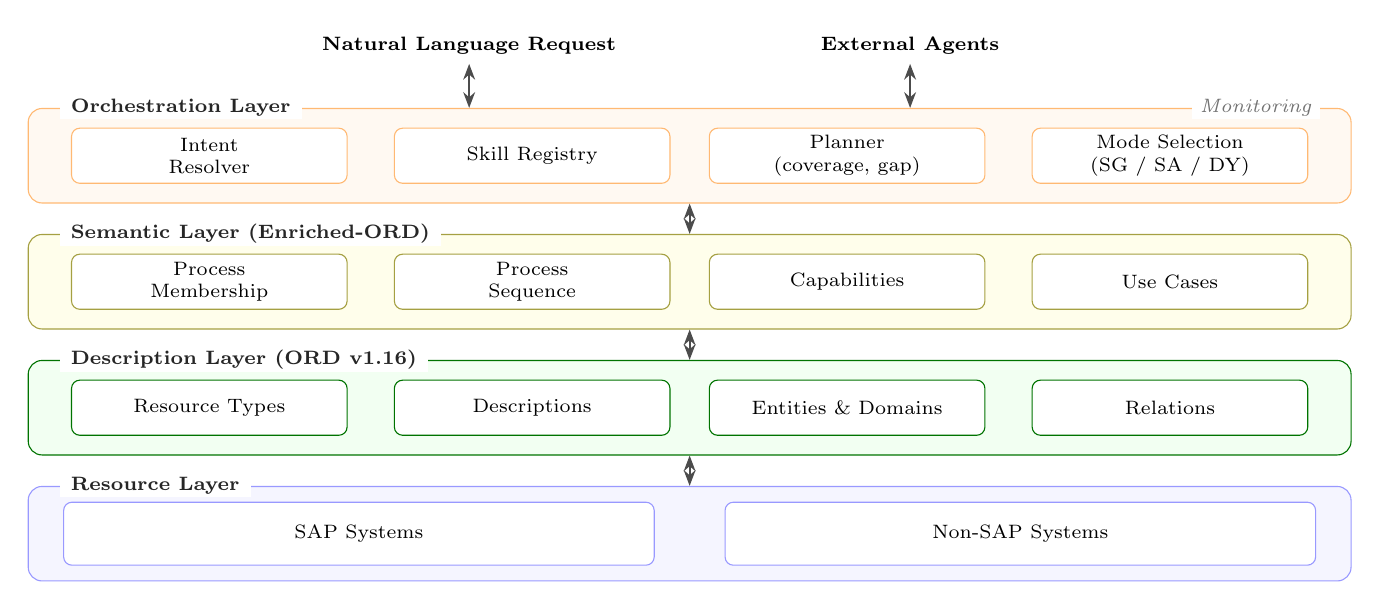
\begin{tikzpicture}[
    font=\footnotesize,
    layer/.style    ={draw, rounded corners=5pt, inner sep=4pt},
    down/.style     ={{Stealth[length=2mm]}-{Stealth[length=2mm]}, thick, draw=black!70},
    llabel/.style   ={font=\scriptsize\bfseries, text=black!85, fill=white, inner xsep=4pt, inner ysep=1pt},
    annot/.style    ={font=\scriptsize\itshape, text=black!55, fill=white, inner xsep=3pt, inner ysep=1pt},
    actor/.style    ={font=\scriptsize\bfseries, align=center},
    compo/.style    ={draw=orange!55, rounded corners=3pt, align=center, minimum height=7mm, inner xsep=3pt, inner ysep=0pt, font=\scriptsize, fill=white},
    compy/.style    ={draw=yellow!60!black, rounded corners=3pt, align=center, minimum height=7mm, inner xsep=3pt, inner ysep=0pt, font=\scriptsize, fill=white},
    compg/.style    ={draw=green!45!black, rounded corners=3pt, align=center, minimum height=7mm, inner xsep=3pt, inner ysep=0pt, font=\scriptsize, fill=white},
    compb/.style    ={draw=blue!40, rounded corners=3pt, align=center, minimum height=7mm, inner xsep=3pt, inner ysep=0pt, font=\scriptsize, fill=white},
  ]
  \node[actor] (user)  at (-28mm, 32mm) {Natural Language Request};
  \node[actor, align=center] (extag) at (28mm, 32mm) {External Agents};
  \node[layer, fill=orange!5, draw=orange!55, minimum width=168mm, minimum height=12mm] (orch) at (0mm, 18mm) {};
  \node[llabel, anchor=west] at ([xshift=4mm]orch.north west) {Orchestration Layer};
  \node[annot,  anchor=east] at ([xshift=-4mm]orch.north east) {Monitoring};
  \node[compo, minimum width=35mm] at ([xshift=-61mm]orch.center) {Intent\\Resolver};
  \node[compo, minimum width=35mm] at ([xshift=-20mm]orch.center) {Skill Registry};
  \node[compo, minimum width=35mm] at ([xshift= 20mm]orch.center) {Planner\\\scriptsize (coverage, gap)};
  \node[compo, minimum width=35mm] at ([xshift= 61mm]orch.center) {Mode Selection\\\scriptsize (SG / SA / DY)};
  \draw[down] (user)  -- (user  |- orch.north);
  \draw[down] (extag) -- (extag |- orch.north);
  \node[layer, fill=yellow!8, draw=yellow!60!black, minimum width=168mm, minimum height=12mm] (sem) at (0mm, 2mm) {};
  \node[llabel, anchor=west] at ([xshift=4mm]sem.north west) {Semantic Layer (Enriched-ORD)};
  \node[compy, minimum width=35mm] at ([xshift=-61mm]sem.center) {Process\\Membership};
  \node[compy, minimum width=35mm] at ([xshift=-20mm]sem.center) {Process\\Sequence};
  \node[compy, minimum width=35mm] at ([xshift= 20mm]sem.center) {Capabilities};
  \node[compy, minimum width=35mm] at ([xshift= 61mm]sem.center) {Use Cases};
  \draw[down] (orch.south) -- (sem.north);
  \node[layer, fill=green!5, draw=green!45!black, minimum width=168mm, minimum height=12mm] (desc) at (0mm, -14mm) {};
  \node[llabel, anchor=west] at ([xshift=4mm]desc.north west) {Description Layer (ORD v1.16)};
  \node[compg, minimum width=35mm] at ([xshift=-61mm]desc.center) {Resource Types};
  \node[compg, minimum width=35mm] at ([xshift=-20mm]desc.center) {Descriptions};
  \node[compg, minimum width=35mm] at ([xshift= 20mm]desc.center) {Entities \& Domains};
  \node[compg, minimum width=35mm] at ([xshift= 61mm]desc.center) {Relations};
  \draw[down] (sem.south) -- (desc.north);
  \node[layer, fill=blue!4, draw=blue!40, minimum width=168mm, minimum height=12mm] (res) at (0mm, -30mm) {};
  \node[llabel, anchor=west] at ([xshift=4mm]res.north west) {Resource Layer};
  \node[compb, minimum width=75mm, minimum height=8mm] at ([xshift=-42mm]res.center) {SAP Systems};
  \node[compb, minimum width=75mm, minimum height=8mm] at ([xshift= 42mm]res.center) {Non-SAP Systems};
  \draw[down] (desc.south) -- (res.north);
  \end{tikzpicture}
  \caption{Reference architecture. The Resource Layer contains heterogeneous enterprise systems. The Description Layer aggregates their ORD metadata. The Semantic Layer extends it with four typed process-derived field groups at design time. The Orchestration Layer resolves requests via Intent Resolver, Skills, Planner, and Mode Selection.}
  \label{fig:architecture-overview}
  \end{figure*}

% (1) Derive requirements from literature and expert interviews.
% (2) Design the reference architecture and its four layers.
% (3) Specify the data flows that populate and use those layers.
% (4) Define the seven retrieval methods that operate within them.

This section presents how the three contributions are constructed. Following the Design Science Research paradigm of Österle et al.\ \citep{osterle2010}, their development iterates between design and evaluation: (1)~the \emph{reference architecture}, which defines a process-aware orchestrator over a typed, semantically enriched resource description layer; (2)~the \emph{retrieval strategies}, which specify seven methods spanning the retrieval families identified in Sec.~\ref{sec:rel-c}; and (3)~the \emph{evaluation setup}, which compares these strategies on ORD-Bench under different description conditions.

\textbf{Design objectives.} The reference architecture is derived from four design objectives that capture the capabilities required for reliable resource selection in heterogeneous enterprise landscapes. These objectives are identified in two stages. First, a systematic analysis of the literature reviewed in Sec.~\ref{sec:rel-c} yields an initial requirement catalogue (Appendix~\ref{appendix:requirements-lit}). Second, these literature-derived requirements are validated and refined through five semi-structured expert interviews with practitioners who develop or operate enterprise orchestration systems; the interview transcripts are documented in Appendix~\ref{appendix:interviews}. The interview data are analysed using Mayring's qualitative content analysis \citep{mayring_qualitative_2014}, with the statement-level coding recorded in Appendix~\ref{appendix:interview-coding}. 

Consolidating both stages yields the final requirement catalogue for the reference architecture (Appendix~\ref{appendix:requirements-final}), grouped into four design objectives: \textit{DO1}—process execution across the full structuredness spectrum; \textit{DO2}—a typed, vendor-neutral resource description layer; \textit{DO3}—semantic enrichment linking business processes to resources; and \textit{DO4}—an orchestration mechanism capable of disambiguating functionally similar resources.


%% Single-column arch figure (kept for reference, currently replaced by figure* below)
%\begin{figure}[t]
%  \centering
%  \resizebox{\columnwidth}{!}{%
%  \begin{tikzpicture}[
%    font=\footnotesize,
%    layer/.style    ={draw, rounded corners=3pt, inner sep=5pt, fill=gray!4},
%    comp/.style     ={draw, rounded corners=2pt, align=center, minimum height=8mm, minimum width=28mm, inner xsep=3pt, inner ysep=0pt, font=\scriptsize, fill=white},
%    llabel/.style   ={font=\scriptsize\bfseries, text=black!85, fill=white, inner xsep=3pt, inner ysep=1pt},
%    retr/.style     ={font=\scriptsize\itshape, text=black!60, fill=white, inner sep=2pt},
%    actor/.style    ={font=\scriptsize\bfseries, align=center},
%    down/.style     ={-{Stealth[length=2mm]}, thick, draw=black!70},
%    bidi/.style     ={{Stealth[length=2mm]}-{Stealth[length=2mm]}, thick, draw=black!70}
%  ]
%  \node[actor] (user)  at (-33mm, 30mm) {NL Request};
%  \node[actor] (extag) at (33mm, 30mm)  {Ext.\ Agents};
%  \node[layer, minimum width=130mm, minimum height=14mm] (orch) at (0mm, 18mm) {};
%  \node[llabel, anchor=west] at ([xshift=4mm]orch.north west) {Orchestration Layer};
%  \node[comp] at ([xshift=-45mm]orch.center) {Intent\\Resolver};
%  \node[comp] at ([xshift=-15mm]orch.center) {Skill\\Registry};
%  \node[comp] at ([xshift=15mm]orch.center)  {Planner};
%  \node[comp] at ([xshift=45mm]orch.center)  {Mode\\Selection};
%  \draw[bidi] (user)  -- (user  |- orch.north);
%  \draw[bidi] (extag) -- (extag |- orch.north);
%  \node[layer, minimum width=130mm, minimum height=14mm] (sem) at (0mm, 0mm) {};
%  \node[llabel, anchor=west] at ([xshift=4mm]sem.north west) {Semantic Layer (Enriched-ORD)};
%  \node[comp] at ([xshift=-45mm]sem.center) {Process\\Membership};
%  \node[comp] at ([xshift=-15mm]sem.center) {Process\\Sequence};
%  \node[comp] at ([xshift=15mm]sem.center)  {Capabilities};
%  \node[comp] at ([xshift=45mm]sem.center)  {Use Cases};
%  \draw[bidi] (orch.south) -- (sem.north) node[retr, midway] {Runtime Retrieval};
%  \node[layer, minimum width=130mm, minimum height=14mm] (desc) at (0mm, -18mm) {};
%  \node[llabel, anchor=west] at ([xshift=4mm]desc.north west) {Description Layer (ORD)};
%  \node[comp] at ([xshift=-45mm]desc.center) {Resource Types};
%  \node[comp] at ([xshift=-15mm]desc.center) {Descriptions};
%  \node[comp] at ([xshift=15mm]desc.center)  {Entities \& Domains};
%  \node[comp] at ([xshift=45mm]desc.center)  {Relations};
%  \draw[down] (desc.north) -- (sem.south) node[retr, midway] {Design-time Enrichment};
%  \node[layer, minimum width=130mm, minimum height=14mm] (res) at (0mm, -36mm) {};
%  \node[llabel, anchor=west] at ([xshift=4mm]res.north west) {Resource Layer};
%  \node[comp, minimum width=56mm] at ([xshift=-30mm]res.center) {SAP Systems};
%  \node[comp, minimum width=56mm] at ([xshift=30mm]res.center)  {Non-SAP Systems};
%  \draw[down] (desc.south) -- (res.north);
%  \end{tikzpicture}}
%  \caption{Reference architecture.}
%  \label{fig:architecture-overview-single}
%\end{figure}


\textbf{Reference architecture.} The reference architecture (Fig.~\ref{fig:architecture-overview}) addresses the design objectives by introducing a process-aware orchestrator. It is structured into four layers.

The \emph{Resource Layer} represents the existing heterogeneous enterprise landscape comprising SAP and non-SAP systems across ERP, HR, manufacturing, and other business domains. It reflects the operational systems found in today's enterprises, which continue to expose their native capabilities unchanged. The proposed architecture does not replace or modify these systems. Instead, it builds upon them, treating their capabilities as the resources selected and invoked by the orchestration layer.



\begin{figure}[t]
  \centering
  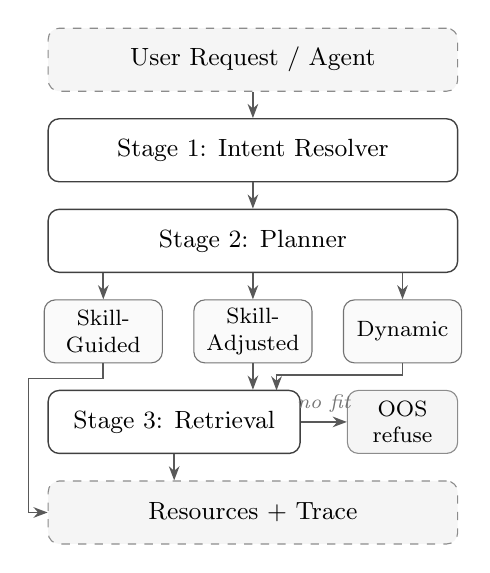
\begin{tikzpicture}[
    font=\small,
    io/.style     ={draw=black!45, dashed, rounded corners=4pt, align=center, minimum height=8mm, minimum width=52mm, inner sep=2pt, font=\small, fill=gray!8},
    stagew/.style ={draw=black!75, line width=0.5pt, rounded corners=4pt, align=center, minimum height=8mm, minimum width=52mm, inner sep=2pt, font=\small, fill=white},
    stage/.style  ={draw=black!75, line width=0.5pt, rounded corners=4pt, align=center, minimum height=8mm, minimum width=32mm, inner sep=2pt, font=\small, fill=white},
    mode/.style   ={draw=black!55, rounded corners=4pt, align=center, minimum height=8mm, minimum width=15mm, inner sep=1pt, font=\footnotesize, fill=gray!4},
    refuse/.style ={draw=black!45, rounded corners=4pt, align=center, minimum height=8mm, minimum width=14mm, inner sep=1pt, font=\footnotesize, fill=gray!8},
    down/.style   ={-{Stealth[length=1.8mm]}, semithick, black!65},
  ]
  % vertical grid: y decreases downward, uniform row pitch
  \node[io]     (rt-in)     at (0,  0)     {User Request / Agent};
  \node[stagew] (rt-intent) at (0, -1.15)  {Stage 1: Intent Resolver};
  \node[stagew] (rt-plan)   at (0, -2.30)  {Stage 2: Planner};
  % three modes
  \node[mode] (rt-sg) at (-1.9, -3.45) {Skill-\\Guided};
  \node[mode] (rt-sa) at ( 0,   -3.45) {Skill-\\Adjusted};
  \node[mode] (rt-dy) at ( 1.9, -3.45) {Dynamic};
  % Stage 3 (narrow) on the left; OOS under Dynamic on the same row
  \node[stage]  (rt-retr) at (-1.0, -4.6) {Stage 3: Retrieval};
  \node[refuse] (rt-oos)  at ( 1.9, -4.6) {OOS\\refuse};
  \node[io]     (rt-out)  at (0, -5.75) {Resources + Trace};
  % spine
  \draw[down] (rt-in) -- (rt-intent);
  \draw[down] (rt-intent) -- (rt-plan);
  % planner fans out to the three modes (straight drops)
  \draw[down] (rt-plan.south -| rt-sg) -- (rt-sg.north);
  \draw[down] (rt-plan.south -| rt-sa) -- (rt-sa.north);
  \draw[down] (rt-plan.south -| rt-dy) -- (rt-dy.north);
  % Skill-Adjusted straight down into Stage 3
  \draw[down] (rt-sa.south) -- (rt-sa.south |- rt-retr.north);
  % Dynamic: down, left, into Stage 3 top
  \draw[down] (rt-dy.south) -- (1.9,-4.0) -- (0.3,-4.0) -- (0.3,-4.2);
  % Skill-Guided bypasses retrieval: down the far left into Resources + Trace
  \draw[down] (rt-sg.south) -- (-1.9,-4.05) -- (-2.85,-4.05) -- (-2.85,-5.75) -- (rt-out.west);
  % Stage 3 to output (straight down)
  \draw[down] (rt-retr.south) -- (rt-retr.south |- rt-out.north);
  % Stage 3 to OOS refuse (horizontal, no fit)
  \draw[down] (rt-retr.east) -- node[above,font=\scriptsize\itshape,text=black!55]{no fit} (rt-oos.west);
  \end{tikzpicture}
  \caption{Orchestration modes. The Planner routes each request to one of three modes; Skill-Guided bypasses retrieval (its resources are pinned in the skill), while Skill-Adjusted and Dynamic resolve unbound steps through Stage~3. When no resource fits, Stage~3 abstains (out-of-scope).} %The design-time flow is in Appendix~\ref{appendix:design-time-impl}.}
  \label{fig:flows}
\end{figure}



The \emph{Description Layer} provides the common representation required to discover and distinguish heterogeneous enterprise resources across system boundaries. Enterprise systems expose system-specific interfaces and metadata that cannot be interpreted uniformly without a shared description format. It therefore represents these resources through Open Resource Discovery (ORD) v1.16 \citep{linux_foundation_europe_open_nodate}. Each system publishes metadata via the read-only ORD Service Provider Interface, which an ORD Aggregator periodically harvests into a single enterprise-wide registry consumable by both AI and conventional applications. Every resource is described through ORD's standard metadata, including resource types, descriptions, entities and domains, and relations. These typed fields provide structural context for resource discovery and initial disambiguation, while ORD additionally specifies the technical information required for invocation, including API protocols, endpoints, and access details. This layer realises \textit{DO2} by providing a typed, vendor-neutral description layer across heterogeneous enterprise systems. Appendix~\ref{appendix:ord-protocol} provides further details on the ORD specification and its resource description model.

The \emph{Semantic Layer} extends the unified description layer with the business context required for reliable resource selection. While ORD provides structural context that helps distinguish resources, it does not capture the process situations and business intents in which a resource represents the appropriate capability. The semantic layer therefore enriches each resource with additional metadata describing its business meaning and applicability. In this work the enrichment is \emph{process-derived}: each enterprise process model from ORD-Bench is matched to the resources realising its steps, and four typed fields (capabilities, use cases, process groups, and process-successor links) are derived from that mapping and written back into each resource. Process models are one possible source; other enterprise artefacts such as organisational models or knowledge graphs could supply the same layer depending on the context available. This layer realises DO3 by linking business processes to resources through this process-derived enrichment.

The \emph{Orchestration Layer} performs runtime resource selection by resolving a natural-language request against available enterprise capabilities and the current context. Rather than reasoning directly over system-specific interfaces, it operates on structured resource descriptions and their semantic enrichment to select the resource best suited to execute the requested capability. The layer comprises four components. The \emph{Intent Resolver} identifies whether the request matches available context artefacts in the Skill Registry and returns the corresponding skill identifier, or \texttt{null} if no matching skill exists. The \emph{Skill Registry} stores Markdown artefacts that provide machine-readable business context for the LLM. These artefacts may contain process knowledge, execution guidance, or other domain-specific information that supports context-aware orchestration. A representative skill artefact is shown in Appendix~\ref{appendix:skill-example}. The \emph{Planner} is invoked when a matching skill exists and determines whether the request is fully covered or requires additional resource discovery. \emph{Mode Selection} then routes execution to one of three orchestration modes. This layer jointly realises \textit{DO1} through process-aware execution across the full structuredness spectrum and \textit{DO4} through runtime selection and disambiguation among functionally similar resources.

\textbf{Orchestration modes.} The orchestrator supports three execution modes covering the full process-structuredness spectrum \citep{van_der_aalst_business_2013,di_ciccio_knowledge-intensive_2015}. Figure~\ref{fig:flows} illustrates how requests flow through the architecture into each mode. The modes describe different interaction patterns between the components of the orchestration layer based on the availability of reusable context and the required degree of runtime resource discovery. \emph{Skill-Guided} (SG) applies when a suitable skill artefact provides sufficient context for execution: the required resources are specified upfront and the request can be handled without retrieval. \emph{Skill-Adjusted} (SA) applies when available context covers only part of the request; the orchestrator follows the guidance where applicable and uses retrieval to resolve uncovered steps. \emph{Dynamic} (DY) applies when no suitable skill exists and resources must be discovered.

\begin{table}[t]
  \renewcommand{\arraystretch}{1.15}
  \caption{Retrieval methods. Baseline is the no-retrieval reference; Agentic Hybrid is the composite. Full detail in Appendix~\ref{appendix:retrieval-code}.}
  \label{tab:methods}
  \centering\small
  \setlength{\tabcolsep}{3pt}
  \begin{tabularx}{\columnwidth}{@{} l X @{}}
  \toprule
  \textbf{Name} & \textbf{Core mechanism} \\
  \midrule
  Free-text Baseline    & LLM call over all resource descriptions \\
  \midrule
  Embedding Cosine      & Cosine similarity over description fields \\
  Progressive Disclosure & Multi-stage LLM filtering \\
  Graph Walk            & ORD graph traversal with LLM reranker \\
  Agentic Tools         & Agent with typed ORD tools \\
  Agentic Raw           & Agent with access over ORD files \\
  Agentic Hybrid  & Agentic loop invoking Embedding, Progressive, and Tools \\
  \bottomrule
  %\multicolumn{2}{@{}l@{}}{\scriptsize $^{*}$Agentic composite combining Embedding, Progressive, and Agentic Tools; see Appendix~\ref{appendix:retrieval-code}.}
  \end{tabularx}
\end{table}

\textbf{Retrieval methods.} When the orchestration layer cannot resolve a request entirely from available context, it must discover suitable resources at runtime (Fig.~\ref{fig:flows}, Stage~3). Retrieval therefore operates over the structured resource descriptions and their semantic enrichment provided by the description and semantic layers. The retrieval methods cover the three retrieval families identified by Xu et al.\ \citep{xu_llm-based_2025}, embedding-based ranking, LLM-guided pre-selection, and graph-based traversal, complemented by three agentic variants and a baseline approach (Tab.~\ref{tab:methods}).

All seven methods operate over the same ORD resource descriptions; they differ only in which ORD fields they read and how. The \emph{Baseline} issues a single LLM call over a flat list of resources (\texttt{ordId}, \texttt{title}, \texttt{shortDescription}) without retrieval, serving as the free-text lower bound. \emph{Embedding} ranks resources by cosine similarity between the query and the ORD text fields (\texttt{title}, \texttt{shortDescription}, \texttt{description}), extended on enriched ORD by the appended semantic fields (\texttt{partOfGroups}, \texttt{processNext}, \texttt{capabilities}, \texttt{useCases}). \emph{Progressive} narrows the candidate pool through multi-stage LLM filtering over the typed ORD fields \texttt{namespace}, resource modality, and \texttt{entityType}. \emph{Graph} walks the typed ORD relations (shared entity types, \texttt{partOfGroups}, integration dependencies, \texttt{processNext}) from anchor resources and re-ranks the neighbourhood with an LLM. The three agentic variants give an LLM agent a tool loop over the landscape: \emph{Agentic Tools} exposes typed ORD query tools (filter by entity type, line of business, capability), while \emph{Agentic Raw} exposes only raw access to the ORD JSON files. Finally, \emph{Agentic Hybrid} composes Embedding, Progressive, and Agentic Tools as callable tools and selects among them per query. Full detail for each method is in Appendix~\ref{appendix:retrieval-code}.

Orthogonal to which mode invokes it, each strategy must also determine whether a suitable resource exists at all. This \emph{out-of-scope} (OOS) condition is not an execution mode but a rejection capability implemented per strategy (a similarity threshold, an explicit \texttt{refuse} action, or confidence-based filtering) and is evaluated separately from the three modes.


\begin{figure*}[t]
  \centering
  \begin{tikzpicture}[
    font=\scriptsize,
    inp/.style={draw=blue!40, rounded corners=2pt, fill=blue!4, minimum width=28mm, minimum height=38mm, align=center, inner sep=3pt, text width=26mm},
    gt/.style={draw=black!35, rounded corners=2pt, fill=gray!4, minimum width=28mm, minimum height=40mm, align=left, inner sep=3pt, text width=28mm},
    mbox/.style={draw=black!35, rounded corners=2pt, fill=gray!3, minimum width=52mm, minimum height=7mm, align=left, inner sep=3pt, text width=52mm},
    ok/.style={draw=green!45!black, rounded corners=2pt, fill=green!5, minimum width=40mm, minimum height=7mm, align=center, inner sep=2pt, text width=38mm},
    fail/.style={draw=red!50, rounded corners=2pt, fill=red!4, minimum width=40mm, minimum height=7mm, align=center, inner sep=2pt, text width=38mm},
    arr/.style={-{Stealth[length=1.0mm]}, thin, gray!60},
  ]
  \node[inp] (input) at (0,0mm) {
    \textbf{User request}\\[2pt]
    ``Which products drive most cost? Material expenses, BOM complexity, supplier benchmarks.''\\[4pt]
    \textbf{Mode:} Dynamic\\
    \textbf{Intent:} Single\\
    \textbf{Skill match:} none\\
    \textbf{Case:} dy-10
  };
  \node[gt] (gt) at (35mm,0mm) {
    \textbf{Ground truth}\\
    \texttt{siemens.plm:}\\
    \texttt{dataProduct:}\\
    \texttt{ProductCost-}\\
    \texttt{Analytics:v1}\\[3pt]
    \textbf{Clean-ORD:}\\
    \textit{title:} Product Cost\\
    \textit{ET:} ProductItem,\\
    \quad Material\\
    \textit{LoB:} PLM\\
    \textit{tags:} cost-analysis\\[3pt]
    \textit{(Enriched fields not\\ used at query time)}
  };
  \draw[arr] (input.east) -- (gt.west);
  \def\xm{86mm}
  \def\xr{138mm}
  \node[mbox] (ms) at (\xm, 24mm) {\textbf{Free-text Baseline:} LLM match ``material+supplier'' picks \texttt{my.mes} analytics};
  \node[fail] at (\xr, 24mm) {\texttt{MaterialCostReconciliation:v1} \textbf{\texttimes}};
  \draw[arr] (gt.east) -- (ms.west);
  \node[mbox] (ma) at (\xm, 16mm) {\textbf{Embedding Cosine:} cosine ranks GT first across all 273 resources};
  \node[ok] at (\xr, 16mm) {\texttt{ProductCostAnalytics:v1} \textbf{\checkmark}};
  \draw[arr] (gt.east) -- (ma.west);
  \node[mbox] (mb) at (\xm, 8mm) {\textbf{Progressive Disclosure:} Stage 1 keeps \texttt{sap.s4}, drops \texttt{siemens.plm}};
  \node[fail] at (\xr, 8mm) {\texttt{BOMCostCompliance:v1} \textbf{\texttimes}};
  \draw[arr] (gt.east) -- (mb.west);
  \node[mbox] (mc) at (\xm, 0mm) {\textbf{Graph Walk:} walk-reranker prefers BOM-titled sap.crm resource};
  \node[fail] at (\xr, 0mm) {\texttt{BillOfMaterialsCost:v1} \textbf{\texttimes}};
  \draw[arr] (gt.east) -- (mc.west);
  \node[mbox] (md) at (\xm, -8mm) {\textbf{Agentic Tools:} ET-filter + capability probes; commits to BOM analytics};
  \node[fail] at (\xr, -8mm) {\texttt{BOMCostCompliance:v1} \textbf{\texttimes}};
  \draw[arr] (gt.east) -- (md.west);
  \node[mbox] (me) at (\xm, -16mm) {\textbf{Agentic Raw:} reads sap.ariba, sap.s4 \texttt{ord.json}; finds no fit, refuses};
  \node[fail] at (\xr, -16mm) {\texttt{refuse} \textbf{\texttimes}};
  \draw[arr] (gt.east) -- (me.west);
  \node[mbox] (mf) at (\xm, -24mm) {\textbf{Agentic Hybrid:} \texttt{embedding\_search} + \texttt{get\_resource}, commits to PLM};
  \node[ok] at (\xr, -24mm) {\texttt{ProductCostAnalytics:v1} \textbf{\checkmark}};
  \draw[arr] (gt.east) -- (mf.west);
  \foreach \n/\y in {ms/24, ma/16, mb/8, mc/0, md/-8, me/-16, mf/-24}{
    \draw[arr] (\n.east) -- (118mm, \y mm);
  }
  \end{tikzpicture}
  \caption{Worked example on one Dynamic case (\texttt{dy-10}, single-intent, clean state): the user request and its ground-truth resource (left), and the resource each of the seven methods commits to (right). Embedding and Agentic Hybrid recover the correct \texttt{siemens.plm} resource; Progressive, Graph, and Agentic Tools lock onto BOM-titled distractors in adjacent namespaces; Agentic Raw reads two ERP systems and refuses. The single-case contrast previews the per-method behaviour that the aggregate results in Sec.~\ref{sec:results} quantify.}
  \label{fig:dy-narrative}
\end{figure*}





\textbf{Evaluation setup.} The architecture and retrieval methods were designed against the requirements and design objectives derived above, which define an ORD-based typed description and semantic layer as the retrieval substrate. ORD-Bench instantiates exactly this substrate: each of its components populates one layer of the reference architecture, and its runtime test cases exercise the three orchestration modes plus out-of-scope refusal (Tab.~\ref{tab:eval-cases}). 

The four ORD-Bench test case families match the orchestration modes one-to-one, so that together they span the full process-structuredness spectrum the architecture targets: Skill-Guided cases correspond to fully-specified processes (a matching skill covers the request), Skill-Adjusted cases to partially-specified processes (a skill applies but leaves gap steps for retrieval), Dynamic cases to unstructured requests (no skill matches), and Out-of-Scope cases to requests no resource can satisfy. Evaluating each family therefore tests exactly the mode designed for that degree of process structure. Because the benchmark is built natively on ORD and ships every resource in both a clean and a semantically enriched state over the same landscape, the effect of semantic enrichment on retrieval can be isolated.


\begin{table}[t]
  \renewcommand{\arraystretch}{1.15}
  \caption{ORD-Bench at a glance. Top: the landscape properties that populate each architecture layer. Bottom: the 110 runtime test cases per mode. Every case is run on both the clean and the semantically enriched description state, giving a $7\times2$ (method $\times$ state) design; the 240 ORD-Bench design-time test cases are evaluated in Appendix~\ref{appendix:dt-results}.}
  \label{tab:eval-cases}
  \centering\small
  \setlength{\tabcolsep}{3pt}
  \begin{tabularx}{\columnwidth}{@{} l c X @{}}
  \toprule
  \multicolumn{3}{@{}l}{\textbf{Landscape} (populates the architecture layers)} \\
  \midrule
  Systems        & 10  & Resource Layer \\
  ORD resources  & 273 & Description Layer \\
  Process models & 30  & Semantic Layer \\
  Skill artefacts & 30 & Skill Registry (\texttt{SKILL.md}) \\
  \midrule
  \multicolumn{3}{@{}l}{\textbf{Runtime test cases} (exercise the orchestration layer)} \\
  \midrule
  Skill-Guided (SG)   & 30 & Routing to a matched skill \\
  Skill-Adjusted (SA) & 20 & Retrieval for gap steps in a skill \\
  Dynamic (DY)        & 40 & Ad-hoc retrieval, no matching skill \\
  Out-of-Scope (OOS)  & 20 & Refusal when no resource fits \\
  \midrule
  \textbf{Total}      & \textbf{110} & \footnotesize $\times\,2$ states $=$ 220 runs per method \\
  \bottomrule
  \end{tabularx}
\end{table}

% --- OLD table (test cases only) kept for reference ---
%\begin{table}[t]
%  \renewcommand{\arraystretch}{1.15}
%  \caption{Runtime test cases from ORD-Bench used in this evaluation. Each case is run twice per method, once on the clean and once on the semantically enriched description state, so every retrieval method is evaluated under a $7\times2$ (method $\times$ state) design. The 240 design-time cases are evaluated in Appendix~\ref{appendix:dt-results}.}
%  \centering\small
%  \setlength{\tabcolsep}{3pt}
%  \begin{tabularx}{\columnwidth}{@{} l c X @{}}
%  \toprule
%  \textbf{Mode} & \textbf{\emph{n}} & \textbf{What it evaluates} \\
%  \midrule
%  Skill-Guided (SG)  & 30 & Routing to a matched skill \\
%  Skill-Adjusted (SA) & 20 & Retrieval for gap steps in a skill \\
%  Dynamic (DY)       & 40 & Ad-hoc retrieval, no matching skill \\
%  Out-of-Scope (OOS) & 20 & Refusal when no resource fits \\
%  \midrule
%  \textbf{Total}     & \textbf{110} & \footnotesize run twice per method (clean + enriched): 220 runs \\
%  \bottomrule
%  \end{tabularx}
%\end{table}

Four properties make ORD-Bench suitable for this study: each case targets a resource surrounded by semantically similar distractors, preventing methods from succeeding through trivial matching; the two description states differ only in the four semantic field groups, allowing measured performance differences to be attributed to enrichment rather than changes in the resource landscape; every distractor was placed adversarially using an explicit ambiguity metric rather than sampled at random, so difficulty is a controlled property of the benchmark rather than an artefact of corpus composition; and a dedicated out-of-scope condition tests each method's ability to abstain when no resource fits, covering the full range from positive retrieval to justified refusal. Figure~\ref{fig:dy-narrative} walks one representative ORD-Bench test case through all seven retrieval methods to make the mechanisms concrete before the aggregate results in Sec.~\ref{sec:results}. The design-time process-matching flow that produces the enriched state and its retrieval results is documented in Appendix~\ref{appendix:design-time-impl} and Appendix~\ref{appendix:dt-results}, with a representative design-time trace provided in Appendix~\ref{appendix:trace-dt-proc002s01}.






% \begin{table}[t]
%   \renewcommand{\arraystretch}{1.15}
%   \caption{Orchestration pipeline accuracy per mode. Skill-Guided has no Planner step. Values in \%.}
%   \label{tab:routing-results}
%   \centering\footnotesize
%   \setlength{\tabcolsep}{3pt}
%   \begin{tabularx}{\columnwidth}{@{} l >{\centering\arraybackslash}X >{\centering\arraybackslash}X >{\centering\arraybackslash}X @{}}
%   \toprule
%   \textbf{Mode} & \textbf{Cases} & \textbf{Intent Resolver} & \textbf{Planner} \\
%   \midrule
%   Skill-Guided  & 30 & 70.0 & --- \\
%   Skill-Adjusted & 20 & 90.0 & Gap-found: 90.0 \\
%   Dynamic       & 40 & 60.0 & Decomp: 45.0 \\
%   \midrule
%   \textit{Weighted avg.} & 90 & 70.0 & --- \\
%   \bottomrule
%   \end{tabularx}
% \end{table}




% ─────────────────────────────────────────────────────────────────────────────
\section{Results}
\label{sec:results}
% ─────────────────────────────────────────────────────────────────────────────

The four-layer architecture of Sec.~\ref{sec:design} was implemented and evaluated on the 110 runtime test cases of ORD-Bench (Tab.~\ref{tab:eval-cases}). The test cases were executed as the architecture prescribes: each request is first routed to the orchestration layer, which then invokes retrieval where the mode requires it. Each case is run on both the clean and the semantically enriched ORD state, so the effect of semantic enrichment is measured per method. The results are then reported by concern: the architecture instantiation, orchestration routing, retrieval strategies, effect of semantic enrichment, out-of-scope refusal, and finally the statistical reliability of the comparison. The 240 ORD-Bench design-time test cases were additionally run to populate the enriched state; their retrieval results corroborate the runtime ranking at a larger sample size and are reported in Appendix~\ref{appendix:dt-results}.





\textbf{Architecture instantiation.} Before reporting the test outcomes, it is worth stating how the reference architecture designed in Sec.~\ref{sec:design} was turned into the concrete system under evaluation, with each layer populated from an ORD-Bench artefact. The \emph{Resource Layer} is the benchmark's landscape of 273 resources across ten enterprise systems. The \emph{Description Layer} is their ORD v1.16 metadata, harvested into a single registry the pipeline queries. The \emph{Semantic Layer} is instantiated by running the design-time process-matching flow over the 30 ORD-Bench process models, which writes the four typed field groups back into the resources and thereby produces the Enriched-ORD state evaluated against the clean one. The \emph{Orchestration Layer} is the runtime pipeline itself: its Intent Resolver, Skill Registry (the 30 derived skills), Planner, and Mode Selection are exercised by the 110 runtime cases. The architecture is thus not evaluated in the abstract but as a working instantiation whose every layer is backed by a benchmark artefact; the remainder of this section reports how well that instantiation performs.


\begin{figure}[t]
  \centering
  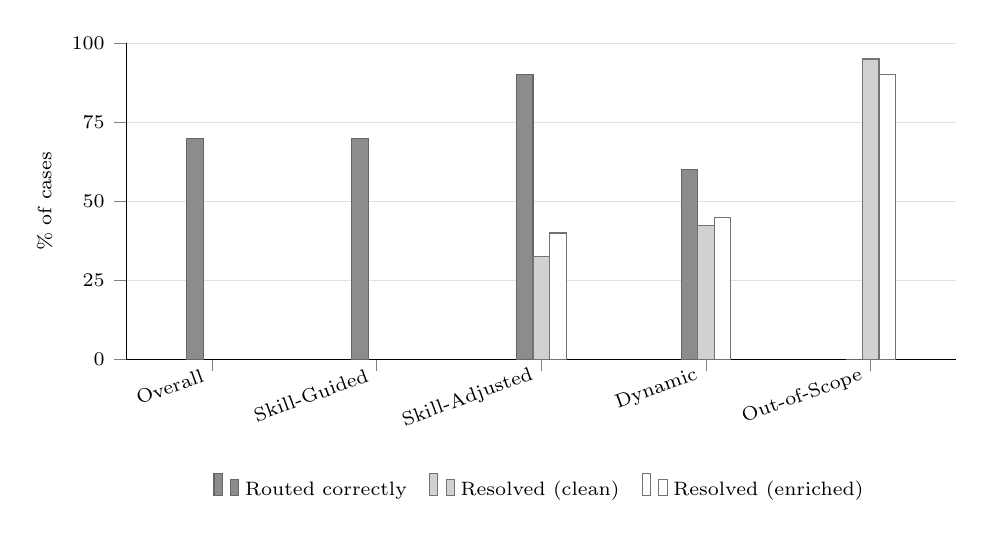
\begin{tikzpicture}
    \begin{axis}[
      width=\columnwidth, height=5.6cm,
      ybar, bar width=6pt,
      symbolic x coords={Overall,Skill-Guided,Skill-Adjusted,Dynamic,Out-of-Scope},
      xtick=data, xticklabel style={font=\scriptsize, rotate=20, anchor=east},
      enlarge x limits=0.13,
      ymin=0, ymax=100,
      ytick={0,25,50,75,100}, yticklabel style={font=\scriptsize},
      ylabel={\% of cases}, ylabel style={font=\scriptsize},
      ymajorgrids, grid style={draw=black!12},
      axis y line*=left, axis x line*=bottom, tick align=outside,
      legend style={at={(0.5,-0.34)}, anchor=north, legend columns=3,
        draw=none, font=\scriptsize, /tikz/every even column/.append style={column sep=6pt}},
      legend cell align=left,
    ]
      \addplot+[fill=black!45, draw=black!60, bar shift=-6pt] coordinates
        {(Overall,70) (Skill-Guided,70) (Skill-Adjusted,90) (Dynamic,60) (Out-of-Scope,0)};
      \addlegendentry{Routed correctly}
      \addplot+[fill=black!18, draw=black!55, bar shift=0pt] coordinates
        {(Overall,nan) (Skill-Guided,nan) (Skill-Adjusted,32.5) (Dynamic,42.5) (Out-of-Scope,95)};
      \addlegendentry{Resolved (clean)}
      \addplot+[fill=white, draw=black!55, bar shift=6pt] coordinates
        {(Overall,nan) (Skill-Guided,nan) (Skill-Adjusted,40) (Dynamic,45.0) (Out-of-Scope,90)};
      \addlegendentry{Resolved (enriched)};
    \end{axis}
  \end{tikzpicture}
  \caption{End-to-end view over the 110 runtime cases. \emph{Overall} (left): combined routing accuracy (70.0\%). Per-mode breakdown (right): dark grey = routing; mid-grey/white = resolution on clean/enriched states, R@1 for Skill-Adjusted (Embedding) and Dynamic (Agentic Hybrid), refusal for Out-of-Scope (Agentic Raw). Overall resolution and Skill-Guided resolution are blank (mixed metrics / no retrieval stage). Stages side by side, not multiplied.}
  \label{fig:funnel}
\end{figure}

\textbf{Orchestration.} Reporting starts from the routing stage, before turning to the individual modes. Figure~\ref{fig:funnel} gives the combined end-to-end view across all 110 cases, placing the routing stage next to the subsequent retrieval stage for the best method per mode. Across the 90 routable cases (SG, SA, and DY; out-of-scope is excluded here, as it has no correct routing target), the Intent Resolver reaches a weighted average routing accuracy of 70.0\% (SA: 90.0\%, SG: 70.0\%, DY: 60.0\%). Routing and retrieval are reported as separate stages rather than multiplied into one number.

The three orchestration modes differ in how far routing alone determines the outcome. Skill-Guided is evaluated by routing accuracy alone: its step resources are pinned in the matched skill, so it bypasses the Planner and Stage~3 entirely. Skill-Adjusted requests are routed most reliably, as they provide stronger contextual signals than exact skill matches. Dynamic requests are the most challenging because distinguishing the absence of a suitable skill from a missed skill match requires reasoning over an open request. Accordingly, the Planner performs reliably when identifying gaps in an existing skill but is less successful at decomposing unstructured requests into the exact set of required sub-queries. Representative runtime traces for Skill-Guided (Appendix~\ref{appendix:trace-rt-sg-03}), Skill-Adjusted (Appendix~\ref{appendix:trace-rt-sa-16}), and Dynamic execution with Agentic Hybrid (Appendix~\ref{appendix:trace-rt-pipeline-dy-21}) illustrate the routing pipeline in Appendix~\ref{appendix:runtime-impl}.


\begin{table*}[t]
  \renewcommand{\arraystretch}{1.15}
  \setlength{\tabcolsep}{0pt}
  \caption{Runtime results for the two retrieval-driven modes. Skill-Guided is omitted as it performs no retrieval (routing only, 70.0\% accuracy, Fig.~\ref{fig:funnel}), and Out-of-Scope is reported separately in Tab.~\ref{tab:oos-results} since it is scored by refusal rather than R@1/R@5. R@1 = recall at rank~1; R@5 = recall within top~5. Ref.\ = OOS refusal rate. $\Delta$ = Enriched $-$ Clean. Bold = best per column. Values in \% (R@1, R@5, Ref.), $\Delta$ in pp. Tokens = average per case.}
  \label{tab:runtime-results}
  \centering\footnotesize
  \begin{tabularx}{\textwidth}{@{} l
      >{\centering\arraybackslash}X >{\centering\arraybackslash}X >{\centering\arraybackslash}X >{\centering\arraybackslash}X >{\centering\arraybackslash}X
      !{\color{black!60}\vrule}
      >{\centering\arraybackslash}X >{\centering\arraybackslash}X >{\centering\arraybackslash}X >{\centering\arraybackslash}X >{\centering\arraybackslash}X
      !{\color{black!60}\vrule}
      >{\centering\arraybackslash}X @{}}
  \toprule
  \textbf{Method}
  & \multicolumn{5}{c}{\textbf{Skill-Adjusted} ($n{=}20$)}
  & \multicolumn{5}{c}{\textbf{Dynamic} ($n{=}40$)}
  & \textbf{Tok.} \\
  \cmidrule(lr){2-6}\cmidrule(lr){7-11}
  & \multicolumn{2}{c}{w/o enr.} & \multicolumn{2}{c}{w/ enr.} & {$\Delta$}
  & \multicolumn{2}{c}{w/o enr.} & \multicolumn{2}{c}{w/ enr.} & {$\Delta$} \\
  \cmidrule(lr){2-3}\cmidrule(lr){4-5}\cmidrule(lr){6-6}
  \cmidrule(lr){7-8}\cmidrule(lr){9-10}\cmidrule(lr){11-11}
  & R@1 & R@5 & R@1 & R@5 & R@1
  & R@1 & R@5 & R@1 & R@5 & R@1 \\
  \midrule
  Baseline
    & 25.0 & 60.0 & 25.0 & \best{60.0} & $\pm$0.0
    & 16.3 & 46.3 & 16.3 & 46.3 & $\pm$0.0
    & 24--44k \\
  Embedding & \best{32.5} & \best{65.0} & \best{40.0} & \best{60.0} & $+7.5$
    & 32.5 & \best{67.5} & 28.7 & \best{70.0} & $-3.8$
    & \best{$\sim$1k} \\
  Progressive & 25.0 & 47.5 & 25.0 & 55.0 & $\pm$0.0
    & 13.8 & 28.7 & 13.8 & 27.5 & $\pm$0.0
    & 6--11k \\
  Graph & 5.0 & 10.0 & 10.0 & 15.0 & $+5.0$
    & 2.5 & 7.5 & 12.5 & 17.5 & $+10.0$
    & 7--12k \\
  Tools & 25.0 & 30.0 & 37.5 & 47.5 & \best{$\mathbf{+12.5}$}
    & 25.0 & 31.2 & 40.0 & 48.7 & \best{$\mathbf{+15.0}$}
    & 75--85k \\
  Raw & 5.0 & 5.0 & 2.5 & 2.5 & $-2.5$
    & 12.5 & 12.5 & 10.0 & 10.0 & $-2.5$
    & 52--141k \\
  Hybrid & \best{32.5} & 60.0 & 30.0 & 50.0 & $-2.5$
    & \best{42.5} & 51.2 & \best{45.0} & 53.7 & $+2.5$
    & 23--36k \\
  \bottomrule
  \end{tabularx}
\end{table*}


\begin{figure}[t]
  \centering
  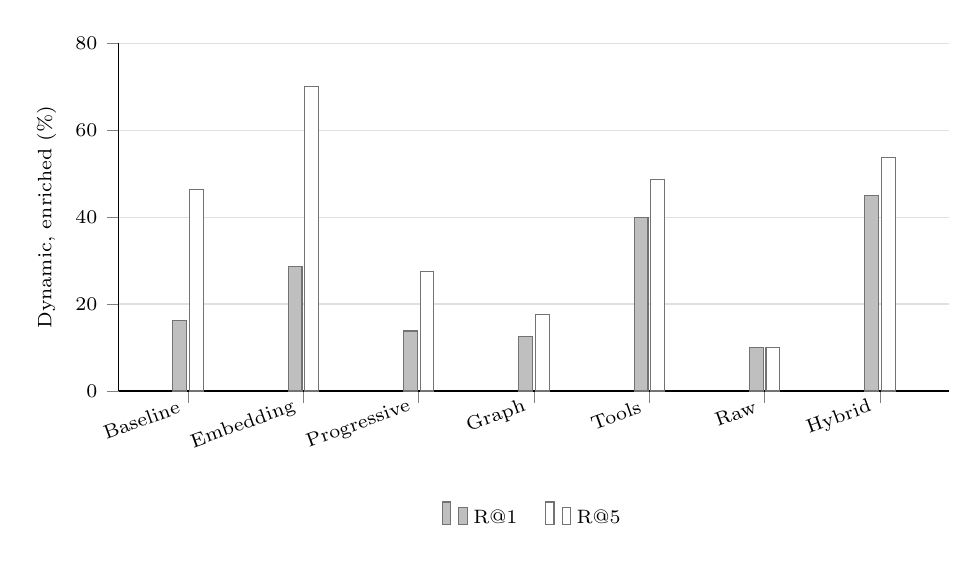
\begin{tikzpicture}
    \begin{axis}[
      width=\columnwidth, height=6.0cm,
      ybar, bar width=5pt,
      symbolic x coords={Baseline,Embedding,Progressive,Graph,Tools,Raw,Hybrid},
      xtick=data, xticklabel style={font=\scriptsize, rotate=20, anchor=east},
      enlarge x limits=0.10,
      ymin=0, ymax=80,
      ytick={0,20,40,60,80}, yticklabel style={font=\scriptsize},
      ylabel={Dynamic, enriched (\%)}, ylabel style={font=\scriptsize},
      ymajorgrids, grid style={draw=black!12},
      axis y line*=left, axis x line*=bottom,
      tick align=outside,
      legend style={
        at={(0.5,-0.30)}, anchor=north, legend columns=2,
        draw=none, font=\scriptsize, /tikz/every even column/.append style={column sep=8pt}
      },
      legend cell align=left,
    ]
      \addplot+[fill=black!25, draw=black!55, bar shift=-3pt] coordinates
        {(Baseline,16.3) (Embedding,28.7) (Progressive,13.8) (Graph,12.5) (Tools,40.0) (Raw,10.0) (Hybrid,45.0)};
      \addlegendentry{R@1}
      \addplot+[fill=white, draw=black!55, bar shift=3pt] coordinates
        {(Baseline,46.3) (Embedding,70.0) (Progressive,27.5) (Graph,17.5) (Tools,48.7) (Raw,10.0) (Hybrid,53.7)};
      \addlegendentry{R@5};
    \end{axis}
  \end{tikzpicture}
  \caption{Rank-1 recall (R@1) versus top-5 recall (R@5) per method on Dynamic under enrichment. The gap is widest for Embedding (28.7 vs.\ 70.0). Typed-field methods (Agentic Tools, Agentic Hybrid) narrow the gap by improving rank-1 accuracy.}
  \label{fig:gap}
\end{figure}

\textbf{Retrieval strategies.} As shown by the orchestration results, retrieval is required only for the two execution modes that discover resources at runtime: Skill-Adjusted and Dynamic. Skill-Guided executes predefined resources and therefore does not exercise the retrieval layer. On these two modes, the best-performing method resolves the correct resource at rank one (recall at rank~1, R@1) in 32.5\% of Skill-Adjusted and 42.5\% of Dynamic cases without enrichment, increasing to 40.0\% and 45.0\% with enrichment (Fig.~\ref{fig:funnel}). These values represent the highest accuracy achieved per execution mode. Table~\ref{tab:runtime-results} reports the results of all retrieval methods on both ORD description states, as R@1 and R@5 (recall within the top~5). The different retrieval strategies are discussed below.

The free-text \emph{Baseline} establishes the reference point, reaching R@1~$\approx$~16--25\% without an explicit retrieval mechanism. \emph{Embedding} improves this by roughly $1.3\times$ on Skill-Adjusted and $2\times$ on Dynamic in the clean state. It also achieves the highest R@5 across all modes (up to 70.0\% on Dynamic with enrichment) while requiring only $\sim$1k tokens per case, making it the least expensive method. Its R@1 changes inconsistently under enrichment, increasing by $+7.5$\,pp on Skill-Adjusted but decreasing by $3.8$\,pp on Dynamic. \emph{Progressive} performs hierarchical candidate filtering over the ORD structure. It requires 6--11k tokens per case and shows no change under enrichment, with R@1 remaining at 25.0\% on Skill-Adjusted and 13.8\% on Dynamic across both ORD states. \emph{Graph} traverses typed ORD relations before re-ranking the results. Under enrichment, its R@1 increases by $+5.0$\,pp on Skill-Adjusted (to 10.0\%) and by $+10.0$\,pp on Dynamic (to 12.5\%). 

The \emph{agentic} methods expose the resource landscape through an iterative tool loop. \emph{Agentic Tools} shows the largest improvement under enrichment, reaching R@1~$=$~40.0\% on Dynamic ($+15.0$\,pp). \emph{Agentic Raw} is both the most expensive method (up to 141k tokens per case) and among the weakest performers. \emph{Agentic Hybrid} achieves the highest Dynamic performance (R@1~$=$~45.0\% with enrichment, more than $2.7\times$ the Baseline) but reaches 32.5\% on Skill-Adjusted, matching the best individual method.

\begin{table}[t]
  \renewcommand{\arraystretch}{1.15}
  \caption{Out-of-scope results ($n{=}20$). $\Delta$ = enriched $-$ baseline on refusal. Embedding and Baseline were evaluated without an explicit refusal mechanism (0\% refusal). Bold = best.}
  \label{tab:oos-results}
  \centering\footnotesize
  \setlength{\tabcolsep}{3pt}
  \begin{tabularx}{\columnwidth}{@{} l
      >{\centering\arraybackslash}X >{\centering\arraybackslash}X
      >{\centering\arraybackslash}X >{\centering\arraybackslash}X
      >{\centering\arraybackslash}X >{\centering\arraybackslash}X
      >{\centering\arraybackslash}X @{}}
  \toprule
  & \multicolumn{2}{c}{\textbf{Refusal Rate}} & \multicolumn{2}{c}{\textbf{False-Pick}} & \multicolumn{2}{c}{\textbf{Avg. Tokens}} & \\
  \cmidrule(lr){2-3}\cmidrule(lr){4-5}\cmidrule(lr){6-7}
  \textbf{Method} & w/o & w/ & w/o & w/ & w/o & w/ & {$\Delta$} \\
  \midrule
  Baseline & 0.0 & 0.0 & 100 & 100 & 15k & 15k & $\pm$0.0 \\
  Embedding & 0.0 & 0.0 & 100 & 100 & \best{1.2k} & \best{1.6k} & $\pm$0.0 \\
  Progressive & 25.0 & 35.0 & 75 & 65 & 5.3k & 5.8k & $+10.0$ \\
  Graph & 65.0 & 85.0 & 40 & 15 & 3.8k & 5.7k & \best{$\mathbf{+20.0}$} \\
  Tools & 40.0 & 45.0 & 60 & 55 & 31k & 40k & $+5.0$ \\
  Raw & \best{95.0} & \best{90.0} & \best{5} & \best{10} & 52k & 22k & $-5.0$ \\
  Hybrid & 15.0 & 30.0 & 85 & 70 & 26k & 25k & $+15.0$ \\
  \bottomrule
  \end{tabularx}
\end{table}



Across all methods, R@5 consistently exceeds R@1: the correct resource is present in the candidate set far more often than it is ranked first, so the bottleneck is ranking rather than coverage. Figure~\ref{fig:gap} visualises this gap across all methods. A breakdown of the Dynamic cases into single- and multi-intent requests is provided in Appendix~\ref{appendix:dy-breakdown}.



\textbf{Out-of-scope.} Out-of-scope cases are scored separately from the retrieval modes above, because success here is the \emph{absence} of a pick rather than a rank: the correct behaviour is refusal, so R@1/R@5 do not apply and refusal rate is reported instead (Tab.~\ref{tab:oos-results}). Graph and the agentic methods carry an explicit \texttt{refuse} action. Agentic Raw refuses most reliably (95.0\% without enrichment, $-5.0$\,pp under it) but at the highest cost; Graph is the most cost-efficient, refusing 65.0\% without enrichment and 85.0\% with it ($+20.0$\,pp) at just 3.7--5.7k tokens; Agentic Tools refuses steadily at 40--45\% and Agentic Hybrid at 15--30\%. Appendix~\ref{appendix:trace-rt-oos-01} provides a representative example trace using Graph Walk. 

Embedding and Baseline provide no rejection mechanism by design and therefore always return a top-ranked resource, leading to false selections on all 20 out-of-scope cases. Confidence-based rejection was evaluated only for methods that natively expose such a mechanism. For Embedding, selecting and validating a similarity threshold is left to future work given the limited sample size, while the Baseline is included as a non-retrieval reference. Possible rejection mechanisms are discussed in Sec.~\ref{sec:discussion}. 


\textbf{Semantic enrichment.} Fig.~\ref{fig:delta-heatmap} visualises the enrichment effect $\Delta = \text{Enriched} - \text{Clean}$ across all methods and modes. The effect divides along how a method consumes the enriched fields. Methods that read them as typed signals improve most: Agentic Tools gains $+12.5$\,pp on Skill-Adjusted and $+15.0$\,pp on Dynamic, and Graph gains $+5.0$ to $+10.0$\,pp on retrieval and $+20.0$\,pp on out-of-scope refusal, its largest single gain. Embedding, which folds the same fields into its text vector rather than reading them as discrete signals, moves in both directions: it gains $+7.5$\,pp on Skill-Adjusted but loses $-3.8$\,pp on Dynamic. Progressive is largely unaffected on retrieval ($\pm 0.0$\,pp on both modes), as its early filtering stages read structure that is identical in the two states, though its refusal does rise ($+10.0$\,pp on out-of-scope). Agentic Raw degrades throughout ($-2.5$\,pp on retrieval, $-5.0$\,pp on refusal), the added capability text giving its unconstrained file reading more plausible-looking but irrelevant material. Semantic enrichment is therefore not uniformly beneficial; its sign depends on the method and the mode.


\begin{figure}[t]
  \centering
  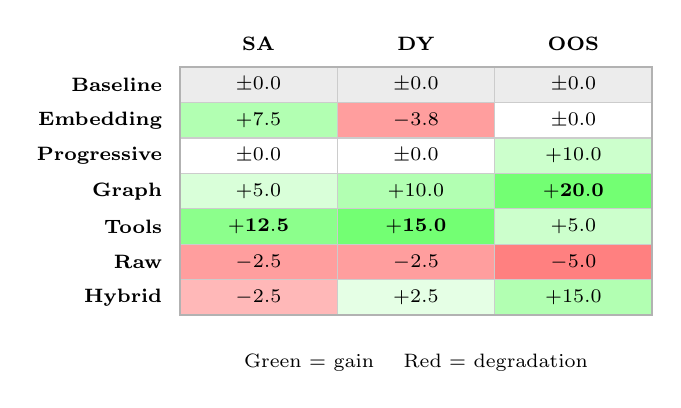
\begin{tikzpicture}[font=\scriptsize]
    \def\cw{20mm}\def\rh{4.5mm}
    \node[font=\scriptsize\bfseries] at (0.5*\cw, 7*\rh+3mm) {SA};
    \node[font=\scriptsize\bfseries] at (1.5*\cw, 7*\rh+3mm) {DY};
    \node[font=\scriptsize\bfseries] at (2.5*\cw, 7*\rh+3mm) {OOS};
    \node[left,font=\scriptsize\bfseries] at (-1mm, 6*\rh+0.5*\rh) {Baseline};
    \fill[gray!15]  (0,6*\rh) rectangle (\cw,7*\rh);   \draw[gray!40] (0,6*\rh) rectangle (\cw,7*\rh);   \node at (0.5*\cw,6.5*\rh) {$\pm$0.0};
    \fill[gray!15]  (\cw,6*\rh) rectangle (2*\cw,7*\rh); \draw[gray!40] (\cw,6*\rh) rectangle (2*\cw,7*\rh); \node at (1.5*\cw,6.5*\rh) {$\pm$0.0};
    \fill[gray!15]  (2*\cw,6*\rh) rectangle (3*\cw,7*\rh);\draw[gray!40] (2*\cw,6*\rh) rectangle (3*\cw,7*\rh);\node at (2.5*\cw,6.5*\rh) {$\pm$0.0};
    \node[left,font=\scriptsize\bfseries] at (-1mm, 5*\rh+0.5*\rh) {Embedding};
    \fill[green!30!white]  (0,5*\rh) rectangle (\cw,6*\rh);   \draw[gray!40] (0,5*\rh) rectangle (\cw,6*\rh);   \node at (0.5*\cw,5.5*\rh) {$+7.5$};
    \fill[red!38!white]   (\cw,5*\rh) rectangle (2*\cw,6*\rh); \draw[gray!40] (\cw,5*\rh) rectangle (2*\cw,6*\rh); \node at (1.5*\cw,5.5*\rh) {$-3.8$};
    \fill[white]          (2*\cw,5*\rh) rectangle (3*\cw,6*\rh);\draw[gray!40] (2*\cw,5*\rh) rectangle (3*\cw,6*\rh);\node at (2.5*\cw,5.5*\rh) {$\pm$0.0};
    \node[left,font=\scriptsize\bfseries] at (-1mm, 4*\rh+0.5*\rh) {Progressive};
    \fill[white]          (0,4*\rh) rectangle (\cw,5*\rh);   \draw[gray!40] (0,4*\rh) rectangle (\cw,5*\rh);   \node at (0.5*\cw,4.5*\rh) {$\pm$0.0};
    \fill[white]          (\cw,4*\rh) rectangle (2*\cw,5*\rh); \draw[gray!40] (\cw,4*\rh) rectangle (2*\cw,5*\rh); \node at (1.5*\cw,4.5*\rh) {$\pm$0.0};
    \fill[green!20!white]  (2*\cw,4*\rh) rectangle (3*\cw,5*\rh);\draw[gray!40] (2*\cw,4*\rh) rectangle (3*\cw,5*\rh);\node at (2.5*\cw,4.5*\rh) {$+10.0$};
    \node[left,font=\scriptsize\bfseries] at (-1mm, 3*\rh+0.5*\rh) {Graph};
    \fill[green!15!white]  (0,3*\rh) rectangle (\cw,4*\rh);   \draw[gray!40] (0,3*\rh) rectangle (\cw,4*\rh);   \node at (0.5*\cw,3.5*\rh) {$+5.0$};
    \fill[green!30!white]  (\cw,3*\rh) rectangle (2*\cw,4*\rh); \draw[gray!40] (\cw,3*\rh) rectangle (2*\cw,4*\rh); \node at (1.5*\cw,3.5*\rh) {$+10.0$};
    \fill[green!55!white]  (2*\cw,3*\rh) rectangle (3*\cw,4*\rh);\draw[gray!40] (2*\cw,3*\rh) rectangle (3*\cw,4*\rh);\node at (2.5*\cw,3.5*\rh) {$\mathbf{+20.0}$};
    \node[left,font=\scriptsize\bfseries] at (-1mm, 2*\rh+0.5*\rh) {Tools};
    \fill[green!45!white]  (0,2*\rh) rectangle (\cw,3*\rh);   \draw[gray!40] (0,2*\rh) rectangle (\cw,3*\rh);   \node at (0.5*\cw,2.5*\rh) {$\mathbf{+12.5}$};
    \fill[green!55!white]  (\cw,2*\rh) rectangle (2*\cw,3*\rh); \draw[gray!40] (\cw,2*\rh) rectangle (2*\cw,3*\rh); \node at (1.5*\cw,2.5*\rh) {$\mathbf{+15.0}$};
    \fill[green!20!white]  (2*\cw,2*\rh) rectangle (3*\cw,3*\rh);\draw[gray!40] (2*\cw,2*\rh) rectangle (3*\cw,3*\rh);\node at (2.5*\cw,2.5*\rh) {$+5.0$};
    \node[left,font=\scriptsize\bfseries] at (-1mm, 1*\rh+0.5*\rh) {Raw};
    \fill[red!38!white]   (0,1*\rh) rectangle (\cw,2*\rh);   \draw[gray!40] (0,1*\rh) rectangle (\cw,2*\rh);   \node at (0.5*\cw,1.5*\rh) {$-2.5$};
    \fill[red!38!white]   (\cw,1*\rh) rectangle (2*\cw,2*\rh); \draw[gray!40] (\cw,1*\rh) rectangle (2*\cw,2*\rh); \node at (1.5*\cw,1.5*\rh) {$-2.5$};
    \fill[red!50!white]   (2*\cw,1*\rh) rectangle (3*\cw,2*\rh);\draw[gray!40] (2*\cw,1*\rh) rectangle (3*\cw,2*\rh);\node at (2.5*\cw,1.5*\rh) {$-5.0$};
    \node[left,font=\scriptsize\bfseries] at (-1mm, 0*\rh+0.5*\rh) {Hybrid};
    \fill[red!28!white]   (0,0*\rh) rectangle (\cw,1*\rh);   \draw[gray!40] (0,0*\rh) rectangle (\cw,1*\rh);   \node at (0.5*\cw,0.5*\rh) {$-2.5$};
    \fill[green!10!white]  (\cw,0*\rh) rectangle (2*\cw,1*\rh); \draw[gray!40] (\cw,0*\rh) rectangle (2*\cw,1*\rh); \node at (1.5*\cw,0.5*\rh) {$+2.5$};
    \fill[green!30!white]  (2*\cw,0*\rh) rectangle (3*\cw,1*\rh);\draw[gray!40] (2*\cw,0*\rh) rectangle (3*\cw,1*\rh);\node at (2.5*\cw,0.5*\rh) {$+15.0$};
    \draw[gray!60, semithick] (0,0) rectangle (3*\cw, 7*\rh);
    \node[font=\scriptsize, align=center] at (1.5*\cw,-6mm) {Green = gain \quad Red = degradation};
  \end{tikzpicture}
  \caption{Enrichment effect $\Delta$ (pp) per method and mode. Agentic Tools gains most in SA and DY ($+12.5$, $+15.0$\,pp); Graph gains most in OOS ($+20.0$\,pp); Embedding degrades on DY ($-3.8$\,pp).}
  \label{fig:delta-heatmap}
\end{figure}


\textbf{Statistical reliability.} With only 20 to 40 cases per execution mode, observed performance differences may reflect sampling variability rather than true differences between retrieval methods. Two complementary analyses therefore assess whether the paper's overarching findings, rather than the exact per-method scores, hold up under this uncertainty.

The first analysis quantifies the uncertainty of each reported score. Resampling the per-case outcomes $10{,}000$ times (\emph{bootstrap}) yields a 95\% confidence interval, the range in which the true performance is likely to lie. On the two strongest methods on Dynamic (enriched, $n{=}40$), Agentic Hybrid reaches R@1~$=45.0\%$ ($[31.2, 58.8]$) and Embedding R@5~$=70.0\%$ ($[57.5, 82.5]$) but only R@1~$=28.7\%$ ($[16.2, 42.5]$). The intervals are wide, so individual scores should not be read to the percentage point, though one qualitative pattern is already visible: no method is best on every metric, as Embedding leads on recall (R@5) and Agentic Hybrid on rank-one precision (R@1). The choice of method thus depends on whether the application needs a broad candidate set or a precise top-one pick.

The second analysis tests two distinct claims that are easily conflated. The first, that \emph{typed retrieval structure} beats free text, is confirmed by a paired McNemar test on the same cases ($p<0.05$ meaning the difference is unlikely to be chance): Agentic Hybrid ($p=0.008$) and Agentic Tools ($p=0.019$) significantly outperform the free-text Baseline. The second and stronger claim, that \emph{semantic enrichment itself} improves selection, requires comparing each method against its own clean-state score. The relevant quantity is the enrichment delta (enriched minus clean R@1), where zero means enrichment changed nothing; a bootstrap interval that stays entirely above zero therefore signals a genuine gain rather than noise. This interval excludes zero for only two methods, Agentic Tools ($+15.0$\,pp, $[+2.5, +27.5]$) and Graph ($+10.0$\,pp, $[+2.5, +20.0]$), precisely the typed-field methods that consume the enriched fields; for the rest the interval spans zero, so no reliable effect can be claimed at this sample size. The evaluation therefore supports two qualitative conclusions, that typed structure beats free text and that enrichment helps the methods aligned to consume it, but not a precise ordering of the strongest methods, which stays within noise ($p>0.15$).

% ─────────────────────────────────────────────────────────────────────────────
\section{Discussion}
\label{sec:discussion}
% ─────────────────────────────────────────────────────────────────────────────

This section first interprets the results with respect to the research question, then examines each contribution in turn (the architecture, the retrieval strategies, the enrichment effect, and the benchmark), before discussing the limitations of the work and directions for future research.

\textbf{Interpretation of findings.} The results show \emph{how} the research question is answered: resource selection is enabled by routing each request to one of three orchestration modes according to its process structure, and by resolving it against a typed ORD description layer rather than free text. Semantic enrichment strengthens selection further, but conditionally: it helps only the retrieval mechanisms whose architecture consumes typed fields, and leaves free-text methods flat or degrades them. The practical implication is that enrichment is not a universal lever. Enterprises should audit their retrieval architecture before investing in metadata enrichment.

\textbf{Process-aware architecture.} The central contribution is the four-layer separation itself: decoupling the resource landscape, its ORD description layer, the process-derived semantic layer, and the orchestration logic is what lets a single pipeline select resources across the full process-structuredness spectrum. Each layer is exercised by the 110 benchmark cases and the ten requirements map cleanly onto the four layers (Appendix~\ref{appendix:requirements-coverage}), so the design is demonstrated end to end rather than only argued for. Its value over prior work is that A-BPMS proposals \citep{dumas_agentic_2026,adimulam_orchestration_2026} defined orchestration layers in increasing detail but left the resource-selection mechanism unspecified, whereas the layered design here supplies exactly that mechanism, and it realises the long-standing SBPM vision of machine-readable process-to-service links \citep{pedrinaci_semantic_2008} without the ontology overhead that limited its adoption, using LLM reasoning over typed ORD fields in place of hand-authored ontologies.

Practitioners confirm both the foundation and the pipeline shape. The architect responsible for the ORD specification notes that its productive use at SAP implicitly confirms the value of a machine-readable self-description layer, and that a unified, consistently-published metadata standard is the prerequisite for any orchestration layer built on top (I2, Appendix~\ref{appendix:interviews}). This productive use underlines the practical value for enterprises of establishing a unified description layer over their resources that can be semantically extended.

\begin{figure}[t]
  \centering
  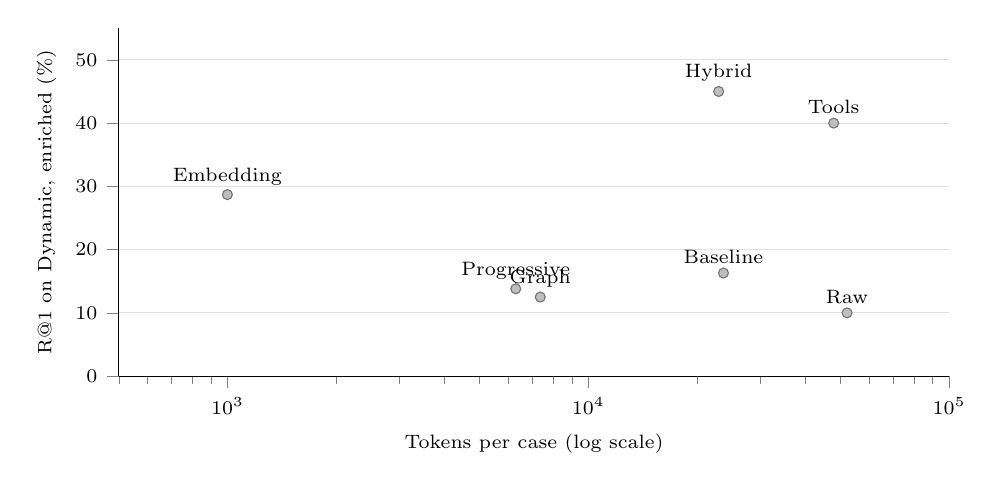
\begin{tikzpicture}
    \begin{semilogxaxis}[
      width=\columnwidth, height=6.0cm,
      xmode=log, log basis x=10,
      xmin=500, xmax=100000,
      xlabel={Tokens per case (log scale)}, xlabel style={font=\scriptsize},
      xticklabel style={font=\scriptsize},
      ymin=0, ymax=55,
      ytick={0,10,20,30,40,50}, yticklabel style={font=\scriptsize},
      ylabel={R@1 on Dynamic, enriched (\%)}, ylabel style={font=\scriptsize},
      ymajorgrids, grid style={draw=black!12},
      axis y line*=left, axis x line*=bottom,
      tick align=outside,
      nodes near coords, point meta=explicit symbolic,
      every node near coord/.append style={font=\scriptsize, anchor=south, text=black},
    ]
      \addplot+[only marks, mark=*, mark size=1.8pt,
                mark options={fill=black!25, draw=black!55}]
        coordinates {
          (999,28.7)  [Embedding]
          (6292,13.8) [Progressive]
          (7359,12.5) [Graph]
          (47859,40.0)[Tools]
          (52117,10.0)[Raw]
          (22969,45.0)[Hybrid]
          (23688,16.3)[Baseline]
        };
    \end{semilogxaxis}
  \end{tikzpicture}
  \caption{Cost--precision trade-off on Dynamic under enrichment: average tokens per case (log scale) versus R@1. Embedding is near-free ($\sim$1k tokens) at 28.7\% R@1; Agentic Hybrid reaches the highest precision (45.0\%) at moderate cost; Agentic Raw is the most expensive yet weakest.}
  \label{fig:pareto}
\end{figure}

Within this architecture, the orchestration layer's routing stage is the clearest gap to production readiness, though the per-mode split is informative. Skill-Adjusted routes most reliably because partially-matching requests carry stronger disambiguation signals, whereas Dynamic is hardest because a genuine ``no skill'' case is difficult to separate from a missed match. Two properties of the layered design soften the impact of routing errors. A Skill-Guided miss falls through to Skill-Adjusted where the Planner compensates, and a Dynamic miss only inflates token cost without affecting which resources are reachable. The design implication is that the structural property of a request should determine the orchestration mode rather than a static routing rule. In production, a confidence threshold that escalates ambiguous requests to the more expensive mode by default, complemented by UX-side clarification when confidence is low, would resolve most remaining routing errors.

\textbf{Retrieval.} No single method dominates and all absolute accuracies stay below production requirements, which follows from ORD-Bench's adversarial construction, where every case is surrounded by semantically close distractors and trivially solvable cases are filtered out. %The free-text methods are bounded by the descriptions themselves, since a description exposes only what its author put in, a limit practitioners confirm (I4, Appendix~\ref{appendix:interviews}), whereas methods that read the typed ORD fields exploit entity types and lines of business as separate filters and pull ahead.

The consistently high R@5 relative to R@1 (Fig.~\ref{fig:gap}) reframes the optimisation target. Recall is already near its ceiling, so the lever is converting existing R@5 into R@1 through a lightweight re-ranking step over the top-five rather than a different retrieval architecture. This is exactly the two-stage shape that two practitioners independently describe, an embedding-based pre-selection narrowed by an LLM decision over the shortlist (I3, I4, Appendix~\ref{appendix:interviews}). %Refusal behaviour is architectural in the same way, as methods without a rejection path false-pick on every out-of-scope case while agentic methods that actively verify abstain reliably, though a similarity cut-off or confidence threshold could add abstention to the former at negligible cost.


\begin{figure}[t]
  \centering
  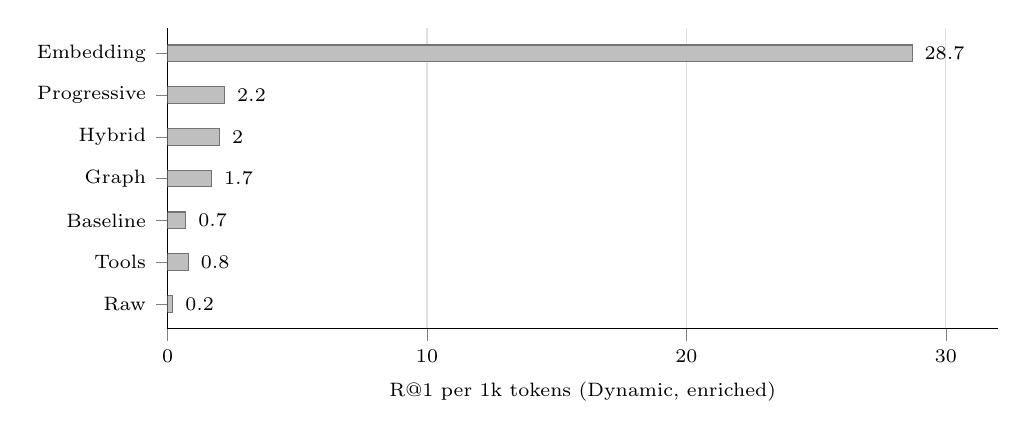
\begin{tikzpicture}
    \begin{axis}[
      width=\columnwidth, height=5.4cm,
      xbar, bar width=6pt,
      symbolic y coords={Raw,Tools,Baseline,Graph,Hybrid,Progressive,Embedding},
      ytick=data, yticklabel style={font=\scriptsize},
      xmin=0, xmax=32,
      xtick={0,10,20,30}, xticklabel style={font=\scriptsize},
      xlabel={R@1 per 1k tokens (Dynamic, enriched)}, xlabel style={font=\scriptsize},
      xmajorgrids, grid style={draw=black!12},
      axis y line*=left, axis x line*=bottom,
      tick align=outside,
      nodes near coords, nodes near coords style={font=\scriptsize, text=black},
      every node near coord/.append style={xshift=1pt, text=black},
      nodes near coords={\pgfmathprintnumber[fixed, precision=1]{\pgfplotspointmeta}},
    ]
      \addplot+[fill=black!25, draw=black!55] coordinates
        {(0.2,Raw) (0.8,Tools) (0.7,Baseline) (1.7,Graph) (2.0,Hybrid) (2.2,Progressive) (28.7,Embedding)};
    \end{axis}
  \end{tikzpicture}
  \caption{Token efficiency: R@1 per 1{,}000 tokens on Dynamic under enrichment. Embedding is more than an order of magnitude more cost-efficient than any other method, since it reaches competitive precision at $\sim$1k tokens. The agentic methods (Agentic Tools, Agentic Raw) buy precision at a steep token cost, and the Agentic Hybrid composite sits in between.}
  \label{fig:token-eff}
\end{figure}

Still, accuracy alone does not decide method choice, since cost varies by more than an order of magnitude across methods. Two views make this concrete. The cost--precision trade-off (Fig.~\ref{fig:pareto}) shows that no method wins on both axes: Embedding is near-free, since it needs no per-query LLM call and only a single query embedding, but scores low on R@1, while the agentic methods buy higher R@1 at a steep token cost through repeated LLM calls. Only Embedding, Agentic Hybrid, and Agentic Tools are not beaten by another method on both cost and R@1 at once, and so represent the sensible choices; the rest are dominated. Token efficiency (Fig.~\ref{fig:token-eff}) sharpens the same picture into a single measure of R@1 per thousand tokens, on which Embedding is more than an order of magnitude ahead of any other method, the agentic methods sit at the opposite end, and Agentic Hybrid falls in between.

Together these views make method selection a deployment trade-off rather than a search for a single winner. A cost-sensitive or high-throughput deployment should default to embedding retrieval and reserve the agentic methods for the cases where their precision gain justifies the cost, a boundary that the growing user tolerance for slower, more deliberate assistants is steadily shifting in favour of the agentic methods (I3, Appendix~\ref{appendix:interviews}).




\textbf{Failure modes.} To characterise why methods fail and derive concrete directions for improving them, every Dynamic case (enriched) was classified by failure type from the per-case traces (Tab.~\ref{tab:failure-modes}). A \emph{rank error} means the correct resource was retrieved into the top five but not ranked first; a \emph{retrieval miss} means it was absent from the candidate set entirely; an \emph{empty return} means the method committed to nothing despite a valid target. 

The value of this breakdown is that each dominant failure mode implies a concrete next step for the affected method rather than a generic call for higher accuracy. Methods dominated by rank errors, need a re-ranking stage over the shortlist rather than better recall, since the target is already present. Methods dominated by retrieval misses, such as the filter-based ones, need their hard early filters softened into soft scores that never prune a namespace to zero. Methods with high empty-return rates need their abstention threshold relaxed or their raw file access replaced with typed tools. The failure profile thus turns each method's aggregate score into an actionable direction for its further development.

\begin{table}[t]
  \renewcommand{\arraystretch}{1.15}
  \caption{Failure-mode breakdown on Dynamic (enriched), as \% of the \emph{failed} cases per method. Rank err. = target in top-5 but not first; Retr.\ miss = target not retrieved; Empty = committed to nothing. Rows sum to 100\% of each method's failures.}
  \label{tab:failure-modes}
  \centering\small
  \setlength{\tabcolsep}{4pt}
  \begin{tabularx}{\columnwidth}{@{} l >{\centering\arraybackslash}X >{\centering\arraybackslash}X >{\centering\arraybackslash}X @{}}
  \toprule
  \textbf{Method} & \textbf{Rank err.} & \textbf{Retr.\ miss} & \textbf{Empty} \\
  \midrule
  Baseline    & 57 & 43 &  0 \\
  Embedding   & 68 & 32 &  0 \\
  Progressive & 28 & 70 &  2 \\
  Graph       & 22 & 65 & 13 \\
  Tools       & 50 & 50 &  0 \\
  Raw         &  2 & 60 & 38 \\
  Hybrid      & 32 & 68 &  0 \\
  \bottomrule
  \end{tabularx}
\end{table}

\textbf{Semantic enrichment.} The most consequential finding is that enrichment is not a universal good. Frameworks such as MCP \citep{noauthor_specification_nodate} and A2A \citep{catalog_ai_nodate} implicitly assume that attaching richer natural-language metadata to a resource makes it easier to select. The evaluation shows the opposite can hold, as the same enriched fields that lift the typed-field methods leave free-text methods flat and actively degrade Embedding. What decides the sign of the effect is not how much metadata is added but whether the retrieval mechanism can address it as structure. A capability filter or a graph edge turns a populated field into a discriminative signal, whereas a single embedding vector folds it back into undifferentiated text and can pull a resource closer to its distractors. Enrichment and retrieval are therefore not independent levers but one coupled design decision.

This reframes the practical question for enterprises from whether to enrich their resource descriptions to whether their retrieval stack consumes typed structure at all. Investing in metadata enrichment without a typed-field retrieval mechanism yields no benefit and may reduce accuracy, so the retrieval architecture should be decided before the enrichment effort, not after. A knowledge-graph practitioner reports the same dependency from production, noting that reliable disambiguation needs use-case- or process-based search over a typed schema rather than plain embeddings, which ``become noisy when multiple resources have similar scope'' (I5, Appendix~\ref{appendix:interviews}). The ORD-Bench paper grounds the mechanism structurally, finding that the identical enrichment lowers structural ambiguity by $-24.5\%$ yet raises embedding cosine by $+27.7\%$ on the same resource pairs, the opposite signs being the structural signature of the mechanism-dependence observed here.

\textbf{Benchmark.} The results hold only under the conditions ORD-Bench enforces. Because every case is adversarially constructed, with the correct resource surrounded by semantically close distractors and trivial cases filtered out, absolute accuracies are lower than an uncurated catalogue would produce, and the ranking between methods is meaningful precisely for that reason. Using ORD-Bench was necessary, since no other benchmark evaluates retrieval over ORD or ships typed enterprise resources in paired clean and enriched states over one fixed landscape. That pairing is what lets this paper isolate the per-method enrichment effect instead of confounding it with a change in the resource set. The study inherits ORD-Bench's assumptions of a synthetic, mid-scale, single-vendor-vocabulary landscape, so the absolute numbers are specific to it while the directional findings are expected to transfer. ORD-Bench is the subject of a dedicated companion paper, which covers its construction and its positioning against prior benchmarks; these are not revisited here.

\iffalse
% Commented out: Paper I has no equivalent "Positioning against related work" paragraph,
% and this one still references the old Cluster A/B/C structure that the reworked Related Work no longer uses.
\textbf{Positioning against related work.} For Cluster~A (service descriptions), the central tension was between expressiveness and adoption: OWL-S and WSMO were expressive enough for automated reasoning but required manual ontology authoring that enterprises never sustained \citep{hepp_ontology_2007}, while OpenAPI achieved broad adoption but left disambiguation to humans. ORD occupies the viable middle ground --- typed enough to support structured retrieval, adopted enough for real-world deployment, and extensible without formal ontologies. The relevant research question is therefore not how expressive descriptions should be, but which structural properties enable which retrieval strategies. The central lesson of the disambiguation analysis --- structural ambiguity $-24.5\%$ but embedding cosine $+27.7\%$ on identical resource pairs --- provides quantitative grounding for why purely description-layer approaches (MCP, A2A) cannot solve the selection problem without architectural alignment on the retrieval side. For Cluster~B (tool retrieval), Tang et al.\ \citep{tang_multi-field_2026} and Lu et al.\ \citep{lu_tools_2026} showed typed fields outperform flat text on synthetic datasets; this work extends their finding to a full enterprise registry that covers APIs, data products, and other resource types together rather than tools alone, under controlled enrichment, and identifies the boundary condition they did not test: enrichment degrades free-text methods. For Cluster~C (agentic BPM), the SBPM vision \citep{pedrinaci_semantic_2008} of machine-readable process-to-service links is realised here without ontology overhead, using LLM reasoning over typed ORD fields instead of hand-authored ontologies. A-BPMS~\citep{dumas_agentic_2026} and Adimulam et al.~\citep{adimulam_orchestration_2026} defined orchestration layers but left the resource-selection mechanism unspecified; this work provides an empirically grounded selection mechanism that spans the full process-structuredness spectrum.
\fi

\textbf{Limitations.} A first group of limitations concerns the preconditions and the method setup. The architecture rests on three preconditions: a unified entity-type vocabulary across system boundaries (e.g., SAP One Domain Model), sufficient ORD metadata coverage, and process models to drive the Skill-Guided and Skill-Adjusted modes. The retrieval methods are deliberately kept untuned, each instantiating one family with a fixed prompt, so that measured differences are attributable to the description layer rather than to optimisation. The absolute numbers are therefore conservative baselines, and more capable implementations of any family (fine-tuned embeddings, calibrated thresholds, learned tool-selection policies) can be expected to raise precision while preserving the enrichment-conditionality finding. All LLM calls used Claude Haiku 4.5; absolute accuracies may shift under stronger models.

A second group concerns evaluation scope and statistical power. The study stops at resource selection and does not measure whether the selected resource executes correctly in a process. ORD-Bench uses LLM-generated resources and single-annotator ground truth without inter-annotator agreement or a held-out partition. At $n{=}20$--40 per split, each 5.0\,pp step is one or two cases, so the intervals are wide and most pairwise differences are not statistically separable (Sec.~\ref{sec:results}). The magnitudes are specific to this landscape while the directional findings should generalise, and larger case counts are the clearest path to decisive results.

A final group concerns the cost of the approach. The semantic ORD extension carries an ongoing burden, since sustaining enriched fields needs maintenance and ownership rules and the four field groups are partly user-defined extensions rather than standardised ORD core.

\textbf{Future work.} On the evaluation side, running more test cases over a larger landscape, which requires scaling ORD-Bench itself, would narrow the wide confidence intervals and make the pairwise method differences statistically decisive. Independent of benchmark scale, the pipeline can be advanced directly: replacing the single-call Intent Resolver with a retrieval-augmented variant, validating the results under a frontier model, and extending the evaluation from resource selection to end-to-end task completion on harnesses such as $\tau$-bench \citep{yao_tau-bench_2024}. The retrieval methods themselves can be pushed further, for instance through learned re-ranking over the top-five shortlist where recall is already high but ranking is not.

On the enrichment side, a dropout-style ablation that removes one field group at a time would isolate which fields carry the disambiguating signal, and a complementary \emph{enriched-only} ablation, exposing the four process-derived fields with the base free-text removed, would isolate their standalone discriminative power and clarify whether the observed embedding degradation stems from mixing typed signal into base text rather than from semantics themselves.

A further direction is also a \emph{self-optimising} orchestrator and retriever that improves during operation rather than relying on fixed logic, a path interviewed practitioners see as the only way to scale across thousands of customised scenarios (I1, I5, Appendix~\ref{appendix:interviews}). Rather than a manually curated intent--resource dataset, such a system could learn from usage signals, explicit feedback or successful downstream execution as rewards. Agentic Hybrid already provides the action space for this, and contextual-bandit formulations that treat each retrieval strategy as an arm offer an established grounding \citep{xu_neural_2020,tang_mba-rag_2025}. The same signals could also refine resource representations through parameter-efficient adapters over a frozen encoder, without altering the descriptions or the deterministic typed-ORD routing \citep{schopf_efficient_2023,gao_simcse_2021}.

% ─────────────────────────────────────────────────────────────────────────────
\section{Conclusion}
\label{sec:conclusion}
% ─────────────────────────────────────────────────────────────────────────────

This work set out to answer the question: \textit{How can a process-aware orchestration architecture and semantic resource descriptions enable resource selection by LLM-based agents in heterogeneous enterprise landscapes?} It addressed this through three contributions, each targeting one of the coordination challenges identified at the outset. (1)~A \emph{process-aware reference architecture} layers a unified ORD description layer and a process-derived semantic layer beneath an agentic orchestration layer with three modes, spanning the full process-structuredness spectrum and thereby supporting coexistence with established processes. (2)~\emph{Seven retrieval strategies} over the typed ORD layer make the trade-off between cost, selectivity, and refusal observable, addressing action-space complexity. (3)~A \emph{systematic comparison} of these strategies with and without semantic enrichment, on 110 ORD-Bench cases.

Together these contributions answer the research question: the process-aware architecture enables reliable resource selection across the full process spectrum, and semantic grounding improves it further, but only for methods whose architecture consumes the typed fields. Structural methods gain up to $+15.0$\,pp under enrichment while free-text methods stay flat or degrade, and the consistently high R@5 shows the architecture reliably surfaces the correct resource in the top five, leaving ranking it first as the remaining challenge. The core lesson is that enrichment and retrieval are one coupled decision: richer descriptions help only where the retrieval mechanism can consume them as structure.

Beyond the technical next steps, the broader trajectory points toward orchestrators executing entire business processes through natural-language intent alone. For this vision, a unified, LLM-accessible description and semantic layer must be in place across all enterprise systems, and this work provides the empirical foundation for that trajectory.

\bibliographystyle{IEEEtran}
\bibliography{../../References/references}

% ─────────────────────────────────────────────────────────────────────────────
\appendix
\onecolumn
\section{Analysis Artefacts}
\label{appendix:analysis}
% ═══════════════════════════════════════════════════════════════════════════

This appendix documents how the requirements that structure the architecture were derived and validated. It proceeds from the literature-derived requirement catalogue, through the five expert interviews and their qualitative coding, to the consolidated final catalogue that the design chapter builds on.

\subsection{Literature-Derived Requirements}
\label{appendix:requirements-lit}

This appendix documents the comprehensive extraction of requirements R1-L to R10-L from the related-work synthesis (Tab.~\ref{tab:requirements-lit}). The catalogue is the deductive starting point for the expert interviews and is built before they are conducted. Each interview statement is later classified against one or more R-L entries as Confirm, Refine, or New (Appendix~\ref{appendix:interview-coding}). The ten requirements are organised under four design objectives DO1--DO4. Each entry records the supporting related-work sources.

\begin{table*}[!t]
\renewcommand{\arraystretch}{1.25}
\caption{Literature-derived requirements R1-L to R10-L, grouped under the four design objectives.}%
\label{tab:requirements-lit}
\centering
\footnotesize
\begin{tabularx}{\textwidth}{@{} l X l @{}}
\toprule
\textbf{ID} & \textbf{Requirement} & \textbf{Sources} \\
\midrule
\multicolumn{3}{@{}l}{\textbf{DO1 --- Process Execution}} \\
\midrule
R1-L & Full process spectrum: structured, repeatable to unmodelled, knowledge-intensive. & \cite{van_der_aalst_business_2013,di_ciccio_knowledge-intensive_2015,aagesen_bpmn_2014,object_management_group_case_2016} \\
R2-L & Procedural knowledge as modular, dynamically loadable skills. & \cite{anthropic_skills_2025,anthropic_agent_harness_2025} \\
R3-L & Agentic execution supports the implementation phase of the BPM lifecycle. & \cite{fettke_business_2025,dumas_agentic_2026} \\
\midrule
\multicolumn{3}{@{}l}{\textbf{DO2 --- Description Layer}} \\
\midrule
R4-L & Resource discovery through a registry with typed structure. & \cite{melzer_service-orientierte_2010,fensel_semantic_2011,linux_foundation_europe_open_nodate} \\
R5-L & Vendor-neutral interfaces enabling interoperability. & \cite{melzer_service-orientierte_2010,noauthor_specification_nodate,noauthor_overview_nodate} \\
\midrule
\multicolumn{3}{@{}l}{\textbf{DO3 --- Semantic Enrichment}} \\
\midrule
R6-L & Machine-interpretable semantics with business meaning. & \cite{mcilraith_semantic_2001,feier_towards_2005,balzer_pitfalls_2004,linux_foundation_europe_open_nodate} \\
R7-L & Lightweight, harvestable description layer without ontology authoring. & \cite{hepp_ontology_2007,pedrinaci_semantic_2008,linux_foundation_europe_open_nodate,sap_se_apeiro_2026} \\
R8-L & Linkage between process model artefacts and IT resources. & \cite{pedrinaci_semantic_2008} \\
\midrule
\multicolumn{3}{@{}l}{\textbf{DO4 --- Orchestration Layer}} \\
\midrule
R9-L & Disambiguate dense action spaces with overlapping descriptions. & \cite{xu_llm-based_2025,gonzalez_gorilla_2024,qin_toolllm_nodate,nizar_agent-as--graph_2026,shi_retrieval_2025} \\
R10-L & Robustness against ``description smells'' at the Semantic Layer. & \cite{hasan_model_2026} \\
\bottomrule
\end{tabularx}
\end{table*}


\subsection{Expert Interviews}
\label{appendix:interviews}

\textbf{Interview guide.} The standardised interview guide corresponds directly to the questions answered by the interviewees in the transcripts below. The guide is built around the literature-derived requirements R1-L to R10-L (Appendix~\ref{appendix:requirements-lit}): each question targets one or more anchor categories so that responses map back to them during coding, while open-ended questions give interviewees room to raise themes the literature did not cover.

\textbf{Transcripts.} The transcripts of the five expert interviews described are reproduced below. Each transcript is preceded by a short profile of the interviewee (role, area, organisational unit) and the date of the interview. Names are anonymised. The transcripts have been lightly edited for readability without changing the content.

\textbf{Participants and selection.} The five interviewees were selected by purposive sampling to cover the roles that jointly shape enterprise agent orchestration: product management, resource-description standardisation, orchestration architecture, product ownership, and knowledge-graph engineering. All build or operate productive agentic systems at SAP, giving between them a view that spans the description layer (ORD), the orchestration runtime (Joule), and the semantic grounding layer (Business Knowledge Graph). Table~\ref{tab:interview-participants} summarises the panel. Each interview followed the same standardised guide, lasted roughly 45--60 minutes, and was conducted between 22~June and 24~July~2026.

\begin{table}[t]
  \renewcommand{\arraystretch}{1.2}
  \caption{Expert interview participants. All roles are at SAP; identifiers I1--I5 are used throughout the coding matrix (Appendix~\ref{appendix:interview-coding}) and the main text.}
  \label{tab:interview-participants}
  \centering\footnotesize
  \setlength{\tabcolsep}{4pt}
  \begin{tabularx}{\columnwidth}{@{} l X l @{}}
  \toprule
  \textbf{ID} & \textbf{Role and area} & \textbf{Date} \\
  \midrule
  I1 & Technical Product Manager, AI Unit (Joule) & 22 Jun 2026 \\
  I2 & Principal Architect, Cross Product Architecture (ORD specification lead) & 30 Jun 2026 \\
  I3 & Area Architect, Joule Orchestration & 01 Jul 2026 \\
  I4 & Area Product Owner, Joule Orchestration & 02 Jul 2026 \\
  I5 & Lead Knowledge Graph Engineer, Business Knowledge Graph & 24 Jul 2026 \\
  \bottomrule
  \end{tabularx}
\end{table}

\subsubsection{Interview --- Technical Product Manager}

\noindent\textit{Role:} Technical Product Manager in the AI Unit at SAP, responsible for Joule. \textit{Date:} 22 June 2026.

\medskip\noindent{\small\textbf{Q1: What is your position? What are you currently building, and what is it meant to do?}}

I am a Product Manager in the AI Unit at SAP. I have been working with AI agents since March 2023, starting right after the release of ChatGPT and early frameworks like AutoGPT. Currently, I am working on Joule, which serves as a generalist agent system. Joule is designed to orchestrate purpose-built expert agents and directly handle user requests across the entire SAP ecosystem, functioning as a broad-scale, overarching agent.

\medskip\noindent{\small\textbf{Q2: What do you see as the main challenges when building or adopting agentic systems in an enterprise context?}}

There are several major challenges. Organisationally, the innovation cycles are extremely fast, making it difficult to keep up and integrate new developments. Technically, the sheer size and breadth of SAP's product portfolio is a massive hurdle. When trying to automate business processes across different products, you immediately run into data quality issues, as well as practical and conceptual problems.

For example, interpreting a user's intent when they ask ``Show me my open items'' or ``Show me my open sales orders'' is incredibly difficult. Objects like ``Sales Orders'' exist in multiple different systems with overlapping definitions. Bringing the right systems together and accurately interpreting intent across such a diverse landscape is highly complex. Additionally, much of the necessary process knowledge currently exists only as undocumented tribal knowledge among employees. Finally, ensuring basic reliability, reproducibility, and safeguarding across these systems remains a constant challenge.

\medskip\noindent{\small\textbf{Q3: When you build an agentic solution, how do you decide what to build and what not to build?}}

We employ a hybrid approach: central teams provide the technology platform, while the Lines of Business build domain-specific expert agents. Initially, this was highly decentralised, which led to collisions, for instance, multiple expert agents claiming to handle ``sales orders,'' leading to ambiguity. We are now shifting towards a more centralised orchestration model to mitigate this.

Regarding use case selection, identification is largely left to the LoBs and is heavily based on perceived business value. However, the quality of these proposed use cases is quite mixed. As we learn to build agents, many proposed use cases are actually strictly deterministic processes. In those instances, it is often more appropriate to use standard automation rather than an agentic system. Currently, there is little systematic methodology to derive the implementation approach directly from the nature of the process itself.

\medskip\noindent{\small\textbf{Q4: How is process knowledge connected to the agent and the actual IT resources that execute the steps?}}

At the moment, process knowledge and the specific IT systems to be connected are mostly hardcoded by developers directly into the agent's code. However, we are finding that this approach is insufficient, particularly for governance and authorisation. Consequently, developers are increasingly required to explicitly document and maintain separate lists of the specific systems and API endpoints their agents use. This allows our authorisation concepts to properly validate and grant access, ensuring that an agent acting on behalf of a user does not exploit all of the user's privileges, but only the explicitly approved ones.

\medskip\noindent{\small\textbf{Q5: How are resources described today?}}

Resources are described using SAP's Unified Meta Data Service via the Open Resource Discovery protocol. Systems and agents both have ORD identifiers. Currently, the wiring between an agent and a system is largely handled via manually created Agent Policies.

\medskip\noindent{\small\textbf{Q6: When an agent needs a resource at runtime, how does it find it?}}

The first step towards automated discovery is having Joule dynamically discover and orchestrate available systems and expert agents that are registered in ORD. We are exploring different retrieval approaches: one relies on self-describing text with minimal metadata, while another constructs a Knowledge Graph from ORD and other UMS metadata to facilitate the retrieval process and return the correct ORD IDs to the orchestrator.

\medskip\noindent{\small\textbf{Q7: How much structure does a resource description need to be reliably usable by an agent?}}

Standardised, central descriptions only go so far because customer landscapes rarely match textbook process models. Every customer has heavy customisations and unique local variants. Therefore, relying entirely on static, structural descriptions is insufficient. The system needs enough structure to identify capabilities, but must rely heavily on dynamic adaptation to handle real-world deviations.

\medskip\noindent{\small\textbf{Q8: Do you see deterministic systems, agents and human tasks coexisting in your landscape?}}

From the orchestrator's perspective, there is no fundamental conceptual difference between a deterministic system (like an RPA or a standard API) and an agent. The orchestrator treats these target systems largely as black boxes. It focuses on what the system can achieve (its capabilities and outputs) rather than how it is implemented internally. The primary challenge in orchestration is not the type of system being called, but rather handling situations where multiple paths can achieve the same goal, and resolving the constraints to find the optimal route.

\medskip\noindent{\small\textbf{Q9: Would machine-readable self-descriptions be useful for an agentic orchestrator?}}

A highly scalable orchestrator cannot rely entirely on manual engineering, it is too complex and does not scale for thousands of customised enterprise scenarios. The architecture must evolve from using generic self-descriptions to becoming a self-optimising system.

\medskip\noindent{\small\textbf{Q10: If you had to build an orchestrator that can reliably disambiguate between similar resources, how would you approach it?}}

Rather than manually defining every step an agent should take, we should define the Definition of Good (target criteria and evaluations). By combining machine-readable metadata (like a Knowledge Graph) with feedback loops, the system can learn from its usage and adapt to local customer realities automatically. This self-optimising approach, fed by initial resource descriptions and continuous feedback, is the only viable way to achieve the required quality and coverage across a massive, customised ecosystem.

\medskip\noindent{\small\textbf{Q11: Further comments or questions?}}

No further comments. The topics discussed cover the core challenges and our current architectural direction.

\subsubsection{Interview --- Principal Architect}

\noindent\textit{Role:} Principal Architect in the Cross Product Architecture Team at SAP, responsible for the Open Resource Discovery (ORD) specification. \textit{Date:} 30 June 2026.

\medskip\noindent{\small\textbf{Q1: What is your position? What are you currently building, and what is it meant to do?}}

I am a Principal Architect in the Cross Product Architecture Team, an organisation that drives architecture alignment across SAP. My focus areas are APIs and events, and specifically specifications and guidelines. The main artefact is the Open Resource Discovery specification, but we also own several other specifications. In general, we take industry standards such as OpenAPI and extend them so that SAP-internal use cases can be covered. We try not to create proprietary standards, but sometimes it becomes necessary because nothing exists yet, ORD itself is an example of that, and it is now around seven to eight years old.

I am also responsible for bridging topics: how to connect API and event architecture to the data product world, and how to connect it to the AI themes.

\medskip\noindent{\small\textbf{Q2: What do you see as the main challenges when building or adopting agentic systems in an enterprise context?}}

The first challenge is having a solid infrastructure foundation, for example, an Agent Gateway that enables centralisation. Simply installing MCP servers locally on every employee's machine will not scale in an enterprise context. You cannot govern that. Investment in good central infrastructure is therefore necessary.

Beyond infrastructure, governance becomes important: who has which permissions, do agents have different rights from the users who trigger them, how can actions be audit-logged, and how can company-wide policies be enforced? From a development perspective, companies also need to maintain an overview of what has been built, what quality standards it meets, and how those standards evolve over time. The entire lifecycle (from execution to continuous improvement) needs to be mastered, roughly the way organisations had to learn DevOps. We now need to do the same for AI.

\medskip\noindent{\small\textbf{Q3: When you build an agentic solution, how do you decide what to build and what not to build?}}

This belongs to the governance process around how we develop. One initial step is to start in planning: there is a planning tool where use cases for agents are captured, described, and reviewed with experts. For a company like SAP it is also important that not only technical and commercial criteria are considered, but also ethical criteria, before significant development begins.

Sometimes the flow is reversed: POCs are built first and then moved into planning. If nothing comes of them, they are discarded. But if the goal is productisation, the use case must pass through a review process. This can be quite democratic, in principle anyone can bring ideas. SAP has kept this process open so that a large number of ideas can emerge quickly, and filtering happens after the broad brainstorming phase.

\medskip\noindent{\small\textbf{Q4: How is process knowledge connected to the agent and the actual IT resources that execute the steps?}}

This belongs on the list of genuinely difficult enterprise governance topics. Getting agents to take company-specific processes into account is related to the audit-logging challenge. At a certain point, a degree of determinism must be introduced in order to maintain compliance.

From SAP's side, we understand standard processes well, and through tools like Process Mining via Signavio we can understand how processes typically run and benchmark which ones operate more efficiently. But ultimately, processes are something the customer defines and adapts. This means there must always be a mechanism for the customer to co-define, restrict, and control what happens. This is one of the hardest topics, and to my knowledge there are no good solutions yet, the whole industry is grappling with it.

To a degree it can be addressed at the API level: the existing backends and transactional logic that SAP already has in its systems can be handed to agents. If agents respect those boundaries, we can carry all of that into the agentic world. But where deterministic compliance is required, the enforcement must happen through APIs, access control, or workflows.

\medskip\noindent{\small\textbf{Q5: How are resources described today?}}

For tools, the current standard is MCP and the way tools are described within MCP. Thinking more broadly, tools are essentially the same as API operations, they can be described as an operation in OpenAPI for REST, or as an Entity Set with access information in OData, depending on the protocol. The key is that all of this is unified centrally through ORD, so that a central aggregator can provide a complete overview of all resources relevant to agents: APIs, native tools via MCP, skills, and other agents. There may also need to be an additional category for contextual information, such as an LLM wiki.

\medskip\noindent{\small\textbf{Q6: When an agent needs a resource at runtime, how does it find it?}}

Discovery currently works in two ways. First, through self-description: an agent or application can expose an ORD endpoint at runtime and describe the resources it provides. Second, for purely static information (such as skills) it is also possible to represent everything via GitHub repositories and handle the ORD publishing behind the scenes. Ideally, applications do not need to implement this themselves. It becomes part of frameworks. ORD has been used productively for discovery within SAP for several years and is now being rolled out much more broadly and with higher priority for the agentic world.

\medskip\noindent{\small\textbf{Q7: How much structure does a resource description need to be reliably usable by an agent?}}

The required structure is protocol-specific (OpenAPI operations for REST, MCP tool descriptions, or Entity Sets in OData) but the unifying factor is that everything ends up in ORD as the shared description layer. Beyond the protocol-level specification, the more important question is company-wide agreement on which metadata standards to use and how they are consistently published, so that a central aggregator can consume them without special-casing.

\medskip\noindent{\small\textbf{Q8: Do you see deterministic systems, agents and human tasks coexisting in your landscape?}}

Workflows are in practice often small microservices with API interfaces for triggering them and for retrieving their output or status. A workflow engine can therefore be described as a system with APIs. Workflow engines such as n8n also expose this via MCP, which brings them back into the same model we already have for other resources.

\medskip\noindent{\small\textbf{Q9: Would machine-readable self-descriptions be useful for an agentic orchestrator?}}

The ORD approach already in use at SAP implicitly confirms the value of machine-readable self-descriptions. Resources describe themselves via ORD endpoints, agents, applications, and MCP servers all expose their capabilities through this standardised description layer, and a central aggregator collects these descriptions and makes them available for discovery. SAP is actively expanding this rollout for the agentic context.

\medskip\noindent{\small\textbf{Q10: If you had to build an orchestrator that can reliably disambiguate between similar resources, how would you approach it?}}

For a reliable orchestrator, the prerequisite is a discovery layer and a company-wide agreement on which metadata standards to use (for example, how OpenAPI is used for REST APIs and how MCP is used within the company) and that all this information can be published consistently. If different applications and teams handle this differently, building a unified orchestration layer becomes very difficult.

As for the aggregator itself, in a very large company one likely reaches a point where the problem must be approached like a data warehouse or ETL challenge, so that the result is a performant layer that consolidates everything and provides a good API for consumers. The critical factor is less about which specific standards are chosen and more about having the mechanisms in place at all. Once everything is collected centrally, the company also gains the ability to apply governance to what has been built, achieve observability, and continuously improve.

\medskip\noindent{\small\textbf{Q11: Further comments or questions?}}

No further comments.

\subsubsection{Interview --- Area Architect}

\noindent\textit{Role:} Area Architect within Joule, responsible for the Orchestration area. \textit{Date:} 1 July 2026.

\medskip\noindent{\small\textbf{Q1: What is your position? What are you currently building, and what is it meant to do?}}

I am an Area Architect within Joule, responsible for the Orchestration area. Simplified, our task is the following: the user says something, and the system has to answer the question of what to do with that input. A simple request such as ``show me tomorrow's weather forecast'' should be relatively straightforward: we have to find an API that returns the weather. But a single user statement can be arbitrarily complex, because it may decompose into multiple tools, tasks, and information sources: different tools, agents, information extracted from documents, a web search, and so on. As an architect, my role is to make sure that all of this comes together coherently, while at the same time supporting the various features that are also expected of the platform.

\medskip\noindent{\small\textbf{Q2: What do you see as the main challenges when building or adopting agentic systems in an enterprise context?}}

The biggest challenge is that we work with content from a wide range of organisations that we do not really control ourselves, or only to a limited extent. There are processes in place to review and validate this content, but realistically, when the content is authored by hundreds of different people, it looks very heterogeneous and does not always match how we envisioned it. As a platform, we can only ship a product that is as good as the content running on top of it, and that is a substantial problem in itself.

From an architecture perspective, the environment is exciting because technologies evolve so quickly, often within six or twelve months, that some things become obsolete, while others that are not yet technically reliable are already visible on the horizon. You cannot sell an enterprise customer on something that does not work today, but you also know that in six months it likely will. Keeping this balance is challenging.

\medskip\noindent{\small\textbf{Q3: When you build an agentic solution, how do you decide what to build and what not to build?}}

The realistic answer is: when the pressure to change is high enough, wherever that pressure comes from, then things get changed. And it is often too late. It is also difficult to throw away existing content, because a lot of people have invested significant time in it and have implemented use cases that they rely on continuing to work in exactly the same way. From an ideal perspective, that content may no longer make sense in a new approach, but the sunk-cost dynamics slow down the transition.

Formal processes for these decisions do not really exist at the moment, although this is starting to change as the Product Management organisation grows and contributes more perspective on what we actually want to support in the future, not just visionary directions, but concrete commitments. In the end, the user does not care whether an MCP server or a direct API sits under the hood. The decision should be driven by what actually creates value for the end user, balanced against what will still be technically relevant a year from now.

\medskip\noindent{\small\textbf{Q4: How is process knowledge connected to the agent and the actual IT resources that execute the steps?}}

Not directly addressed. Related aspects are covered under Q9 and Q10, where the interviewee argues that process knowledge should be part of a central graph rather than hardcoded into skills or agent code.

\medskip\noindent{\small\textbf{Q5: How are resources described today?}}

The main content-delivery concept in the current tool stack is the notion of Joule Functions, which split into so-called Scenarios and Dialog Functions. Scenarios carry the semantic metadata that describes what a given Dialog Function can do. To stay with the weather example, the scenario contains a description (``this is the weather scenario''), a more detailed description (``I can show you the weather for the next week''), and a list of slots such as location or day. The Dialog Function itself only handles the execution and calls the backend system. For orchestration, the scenarios are what matters. Today, we describe both agents and various tools through this scenario mechanism. It is the main way executable content enters the system, and executable content in practice is almost always wired through an API.

In addition to that, we have documents. Through Document Grounding, arbitrary text can be indexed, customer help documents that are exposed via SAP Help, policy documents, and effectively anything that internal groups such as SAP IT consider knowledge-relevant. These are uploaded into Joule, indexed in chunks in Document Grounding, and retrieved through embedding search. Beyond that, there are custom tools available to the Tool Agent, for example a web search, but there is no formal delivery model for those yet, they are integrated ad hoc.

Scenarios are almost entirely authored by the Lines of Business (roughly 99.9\%), with only a handful of defaults provided centrally. Customers can also register their own scenarios. If a customer wants to expose an internal API, for example a canteen menu endpoint, through Joule, they can write their own scenarios to bind that API. The same applies to non-SAP systems that a customer wants to integrate.

\medskip\noindent{\small\textbf{Q6: When an agent needs a resource at runtime, how does it find it?}}

The retrieval process distinguishes a pre-selection step from the actual orchestration decision. Pre-selection for both documents and scenarios runs on semantic similarity via embeddings. For documents, this happens at chunk level. For scenarios, similarity is computed between a rewritten user query and the scenario's description together with representative example sentences. If the user says ``show me the weather'', we may rewrite this into ``show the weather for the user's current location'' and match embeddings against scenario descriptions and document chunks. Pre-selection returns roughly ten scenarios plus a set of chunks, which then enters the core orchestration step. There, one or more LLM calls decide, based on that pre-selected information, which scenario to actually invoke and whether the retrieved document chunks are relevant at all. Once the scenario is selected, the underlying API is called.

There are ambitions to evolve this. What I described corresponds to the internal codename V-4. A follow-on line, currently referred to as V-10, moves toward a more classical agentic behaviour with a ReAct-style loop and a computer-using harness. The idea is to use progressive disclosure: the LLM is asked multiple times, each time seeing a different level of detail, and it can invoke additional tools, for instance a document-based question that returns further documents through embedding or other indexing methods. This direction is being pushed toward general availability. Part of the motivation is that user expectations have shifted. Developers have grown used to waiting longer for tools like Claude Code, and enterprise users of similar tools no longer expect a two-second answer for complex questions. That makes ReAct-style loops more realistic in practice than they were before.

\medskip\noindent{\small\textbf{Q7: How much structure does a resource description need to be reliably usable by an agent?}}

Implicitly addressed under Q5, Q6, and Q10. In the current V-4 stack, the minimum structure per scenario is a short description, a detailed description, a set of representative example sentences, and a slot list. This is what pre-selection matches against. Q10 argues that this baseline is insufficient for reliable disambiguation at scale and that semantically connected information over a graph is required in addition, so that relationships between resources (value helps, dependencies) become explicit rather than left to embedding similarity.

\medskip\noindent{\small\textbf{Q8: Do you see deterministic systems, agents and human tasks coexisting in your landscape?}}

Not directly addressed.

\medskip\noindent{\small\textbf{Q9: Would machine-readable self-descriptions be useful for an agentic orchestrator?}}

Yes, definitely. This aligns with the Knowledge Graph ambitions within SAP more broadly. In my view, the big problem with these systems is discovery: how do I find out which options are available to me at all, without having to pump everything I have into the LLM context, which is expensive, slow, and simply not enough. Doing this discovery efficiently and well is where the different approaches diverge, but in most cases they end up depending on having good, semantically connected information about the systems you are working with. ORD is one approach that carries partial semantic information and dependencies between resources, and at least parts of the discovery are expected to run through ORD, or through the Field Customer Landscape more broadly, so that discovery gets unified. Joule's orchestration is not the only stakeholder with this requirement: many other systems such as Signavio also need to know which APIs exist in a customer's landscape and what they actually look like. Extensibility is a huge topic for SAP customers, and it is what differentiates SAP from any arbitrary ERP startup: Nestl{\'e} does not simply run one SAP system out of the box.

\medskip\noindent{\small\textbf{Q10: If you had to build an orchestrator that can reliably disambiguate between similar resources, how would you approach it?}}

Ignoring cost constraints for a moment, the ideal system would have a fast-answer mode: an LLM path with minimal ceremony, no large sandbox, and short response time. But when a request looks business-relevant, several discovery processes should start in parallel to feed the actual reasoning harness, most likely a computer-using harness that can also write code and act on tools. Part of that discovery must return the available APIs, ideally via a knowledge graph, because this is not just a semantic question but also a relationship question: which API provides a value help for another one, which additional API can I offer alongside a given one, this is expressed most naturally over a graph.

Process information must also come out of such a graph, because as a user I want to describe the result I want, not the process that leads to it. The orchestrator should know that process itself. When I create a purchase order, Joule should know what is needed to create a purchase order in our business system, including that, for example, an email has to be sent to my L+2 manager because that manager must approve every purchase order. I should not have to tell it to send the email as an additional step. That is the optimum. We are still fairly far away from it in many cases, but topics such as EKX and others are moving in that direction.

Alongside APIs and processes, information such as policies and company knowledge should be retrieved in parallel and handed to the harness as the starting point: here is what the user wanted, here is the base information, here are also skills that describe parts of these processes in more detail, please return the following result. Skills as they exist today are a step in that direction. They capture semantic knowledge of how things fit together. But strictly, that kind of knowledge should not be delivered through skills. It should sit centralised in a graph so the individual pieces are better connected. We are not there yet either. The typical architect's mindset applies: you are always fighting against constraints, and it is hard to describe the truly optimal world because you rarely have the chance to build it. That said, this direction would create the biggest value for users, even though under current technology it becomes very expensive: a single weather query at thirty cents is not something anyone wants to pay for.

\medskip\noindent{\small\textbf{Q11: Further comments or questions?}}

No further comments.

\subsubsection{Interview --- Area Product Owner}

\noindent\textit{Role:} Area Product Owner for Joule Orchestration at SAP. \textit{Date:} 2 July 2026.

\medskip\noindent{\small\textbf{Q1: What is your position? What are you currently building, and what is it meant to do?}}

I have been Area Product Owner for Joule Orchestration for about two and a half months. The role covers portfolio work, driving innovation into the team, translating solution-oriented requirements aligned with Product Management into integration patterns and backlog items. I share the area with the Area Architect: he takes the architecture part, I take the Product Owner side for natural-language orchestration.

\medskip\noindent{\small\textbf{Q2: What do you see as the main challenges when building or adopting agentic systems in an enterprise context?}}

The biggest challenge in orchestration, and around it, is evaluation. With the rapid advancements in the AI space, many possible solutions surface, and patterns eventually stabilise in a certain direction, but the challenge is measuring how well they perform. In an SAP product like Joule, orchestration adds further complexity because it faces real-world requirements that go beyond laboratory conditions. A concrete example is multi-system: a customer may have the same system twice, which effectively adds an orchestration problem on top of the actual orchestration problem, so the complexity keeps multiplying.

Having a benchmark for each of these situations is what is missing today. There are many solutions, but identifying the technically best and best-evaluated one, translating it into a product roadmap, and handing the implementation to the teams is currently the biggest challenge.

Regarding evals as they exist today: there is no streamlined approach, they are quite scattered. There are Agent Evals, Knowledge Graph Evals in Joule, and prompt-level tests. On a test pyramid, prompt tests sit at the unit-test level: each LLM call in a product like Joule has a task-descriptive system prompt, and prompt tests define an expected output per LLM call and per orchestrator task. On that level the teams are reasonably well set up. It becomes harder in a distributed system where several specialised prompts talk to each other before converging on a final result. Communication overhead and complexity between the intermediate steps and the final result grow exponentially there. The most prominent internal tool for end-to-end testing today is Golden Dataset Studio, currently with a strong focus on the Knowledge Graph, working with boundary conditions of the form ``as a user I input X and expect Y end-to-end''. Test cases are still curated manually, often by LoB-specific consultants, so statistically the data volume is small.

\medskip\noindent{\small\textbf{Q3: When you build an agentic solution, how do you decide what to build and what not to build?}}

For Skills or MCP the problem is mostly an integration problem rather than an orchestration problem, because most orchestration problems are already solved. It is the surrounding aspects that matter: integration, ownership, sustainability. MCP was top of mind maybe half a year ago and is already partially eclipsed by the ongoing discussion around alternatives like Agent Skills, even though the two can be complementary. From a product management perspective, the biggest challenge is keeping up with the market speed while maintaining product fit. This directly ties into a benefit-versus-effort question: can we afford to spend six months rebuilding Joule Orchestration for a new technology shift, knowing that in another six months something new may appear? Balancing this is essential, and the current process is largely: build a PoC, review it internally, run the unit-test-level prompt tests where applicable, hand it to LoBs for end-to-end feedback, and then decide together whether it warrants strategic productisation.

\medskip\noindent{\small\textbf{Q4: How is process knowledge connected to the agent and the actual IT resources that execute the steps?}}

There is a stark difference between standard processes that ship with SAP standard software and highly customised processes on the customer side. For standard processes, the first challenge is: where can it be found and how well is it consumable for an AI? An early step here was Conversational Search, which enabled a tool on SAP Help documentation and pulled relevant chunks via embedding retrieval into the LLM context to answer questions. This works for standard processes such as leave approval in SuccessFactors or a purchase-order creation, which are documented well enough for customers. It works less well when the content is not rich, when tables or figures are involved, or when formatting breaks the translation. Consumability for AI is then poor.

The next step was to solve this through a Knowledge Graph, though the current graph focuses less on process knowledge and more on the structure of backends and OData APIs. This will likely change and increasingly include process knowledge. The current Canonical Knowledge Graph, however, still only reflects SAP-standard knowledge. The actual value for a customer sits in their modified, customer-specific processes, and this requires a customer-specific or tenant-specific KG. That is technically challenging, and to my knowledge there is not yet a strong communication between the KG teams and the process-modelling side (Signavio) about how tenant-specific process knowledge would be accessed. EKX has strong Signavio integration, but it is Canonical, that is, SAP-standard. There is no scenario yet along the lines of ``my Joule runs on Mercedes-Benz processes at Mercedes-Benz.'' Around 90\% of what we work on in AI is fundamentally integration, not the AI itself. The technical solutions largely exist, evaluation is the missing piece, and before evaluation, technical integration is the missing piece to enable this end-to-end.

\medskip\noindent{\small\textbf{Q5: How are resources described today?}}

In the classical tool stack that is not yet migrated to Agent Skills, resources are exposed through Tool Scenarios, which act as a semantic interface for a function. A scenario carries a name, a description, and parameters. This is essentially the JSON-based tool-calling standard used from the early days, treated here as a semantic interface. Currently, it is up to individual LoBs or content creators to decide what semantic information they place in a scenario. In practice, some LoBs treat this well. Others overload it, effectively scripting the interaction as ``if the user says X, do Y, then say Z'', which is brittle and overfits to a specific prompt and model version. Scenarios in this stack are the mechanism for transactional operations such as posting a purchase order or creating a sales order. Each LoB uses the same framework to expose their backend functionality as a natural-language interface. On top of that, Conversational Search is modelled as a tool as well: it exposes a preview of chunks and offers the orchestrator the option to invoke this tool for informational use cases such as ``what is the maximum lead distance for supplier XYZ''. Together, these two mechanisms provide the semantic surface on which the orchestrator makes its decision.

\medskip\noindent{\small\textbf{Q6: When an agent needs a resource at runtime, how does it find it?}}

For discovery, the orchestrator does not scan all tools. A Preselection step reduces the search space first. Preselection is one of the earliest mechanisms in Joule and was introduced when the context window was still around 16K tokens and everything had to be aggressively optimised. Preselection performs vector embedding matching between a context-rewritten user query, made independent of the conversation history, and each scenario description. It cuts down to the top N scenarios, and only these enter the orchestrator's context for the final selection call.

\medskip\noindent{\small\textbf{Q7: How much structure does a resource description need to be reliably usable by an agent?}}

The observation across LoBs is that the amount of semantic content in a scenario description varies widely. Some LoBs describe their scenarios cleanly at the semantic level. Others write near-scripts inside the description, which overfits to a specific prompt and model. In either case, the orchestrator has only what the scenario description exposes, so quality bounds selection quality directly.

\medskip\noindent{\small\textbf{Q8: Do you see deterministic systems, agents and human tasks coexisting in your landscape?}}

Yes, they coexist. A Tool Scenario can encapsulate a state-machine-driven process, so once it is invoked the deterministic flow runs regardless. The problem is that the flow becomes semantically inflexible. A concrete example: SuccessFactors exposes a scenario ``View Direct Reports''. If the user asks ``How many direct reports does Dominik have?'', the orchestrator correctly picks the scenario. But the LoB implementation renders a list of direct reports rather than answering ``you have twelve.'' The scenario controls the conversation flow from the moment it is invoked but cannot do so context-aware, because it does not see the surrounding conversation. This is a legacy from earlier chatbot patterns where the tool function owned and drove the conversation flow itself. An LLM-based design that reasons over the state machine with full context would handle these cases better.

\medskip\noindent{\small\textbf{Q9: Would machine-readable self-descriptions be useful for an agentic orchestrator?}}

The idea is strong, provided it is adopted broadly and recognised as a standard across the ecosystem. If that happens, ORD becomes consumable by essentially any AI client, which is a major advantage. The current issue is adaptation: as long as adoption is partial, the value is limited. Once the gap is closed, it becomes clearly attractive for Joule, because a client would get out-of-the-box access to semantic knowledge for many systems.

The open question is how tightly to bind the orchestrator to any single description standard, because the landscape has moved through several standards in quick succession (function-calling schemas, MCP, Agent Skills, agent CLIs). Architecturally, the orchestrator should sit at an abstraction level that can absorb such changes. That said, if a strong push commits to a standard such as ORD and it can be shown that Joule benefits from consuming it natively, it becomes a clear PoC candidate. The evaluation question comes back once more: if benefits can be quantified end-to-end, adoption follows.

\medskip\noindent{\small\textbf{Q10: If you had to build an orchestrator that can reliably disambiguate between similar resources, how would you approach it?}}

The direction the orchestrator moves in is a proper agent harness rather than the earlier chatbot-style pattern, including a computer-using variant of the harness (as pursued in the V-10 line). New possibilities open up in that direction: hybrid discovery that combines a filesystem search with additional retrieval steps, and using progressive disclosure to realise preselection through the agent loop itself rather than as a separate pre-orchestration stage. The trade-off is always cost versus benefit: the current preselection is optimised for speed because it runs on every request. Its role was to accelerate the easy, semantically obvious cases so the orchestrator does not have to run a full discovery loop every time. There is clearly appetite to change how this works, especially as Agent Skills arrive as a content format. The concrete algorithmic shape is not fixed, but the architectural direction is clear.

The broader challenge is doing product engineering in an environment where the technology shifts every few weeks. It requires a mindset shift, robust processes, and an architecture that can absorb changes rather than being rebuilt from scratch each time. Only then can the team iterate quickly. Today, before one release is out, the next paradigm is already surfacing, which makes sustainable product engineering very hard. Where in the Gartner Hype Cycle the industry currently sits is difficult to say. The peak seems unusually stretched, and the model itself may no longer apply cleanly.

\medskip\noindent{\small\textbf{Q11: Further comments or questions?}}

No further comments.

\subsubsection{Interview --- Knowledge Graph Engineer}

\noindent\textit{Role:} Lead Knowledge Graph Engineer at SAP, responsible for the Business Knowledge Graph (BKG) and its integration with Joule. The BKG provides semantically rich context for Joule to answer questions based on grounded SAP metadata. \textit{Date:} 24 July 2026.

\medskip\noindent{\small\textbf{Q1: What is your position? What are you currently building, and what is it meant to do?}}

Lead Knowledge Graph Engineer at the Business Knowledge Graph. Currently building the SAP Knowledge Graph and its integration with Joule. It is meant to provide semantically rich context for Joule to answer questions based on grounded SAP metadata.

\medskip\noindent{\small\textbf{Q2: What do you see as the main challenges when building or adopting agentic systems in an enterprise context?}}

The nondeterminism of agentic systems often works against what we are trying to achieve by standardising metadata in a single system. Agents can often see the data, but large context windows for complex queries reduce accuracy; running over multiple calls increases latency, which we are bound to commercially; and longer context increases cost. All of this affects commercial viability.

\medskip\noindent{\small\textbf{Q3: When you build an agentic solution, how do you decide what to build and what not to build?}}

Not directly building an agentic system in my current role.

\medskip\noindent{\small\textbf{Q4: How is process knowledge connected to the agent and the actual IT resources that execute the steps?}}

Process knowledge is often encoded in BPMN diagrams or other structured data formats. In the SAP Knowledge Graph, process knowledge is represented as nodes and edges connecting a process step to an application or API. These steps can be queried by an agent to better understand how to navigate best-practice processes and which APIs to execute.

\medskip\noindent{\small\textbf{Q5: How are resources described today?}}

Not directly owning an agent, but the project contributes to passing metadata to many agents. Resources are often described through skills generated directly from Knowledge Graph data to better guide the agent towards its target.

\medskip\noindent{\small\textbf{Q6: When an agent needs a resource at runtime, how does it find it?}}

At runtime an agent should have access to the list of tools within its own formation, scoped to the use cases it can solve. As tools grow in number and scope, and as responsibilities overlap, managing the tool discovery layer becomes critical to guide the agent to the best option while reducing cost from redundant calls. As more agents and tools are created, this creates a search space problem that must be handled by smart tool discovery design.

\medskip\noindent{\small\textbf{Q7: How much structure does a resource description need to be reliably usable by an agent?}}

Agents need data that is structured rather than just verbose text describing relations. If agents are running multi-step operations and reasoning over which paths to take, a good structure describing possible outcomes is relevant. In the SAP Knowledge Graph, agents (such as the BDC KG Reasoner) can query the graph and decide which path to continue in a step-wise fashion. This allows the agent to navigate complex landscapes with flexibility.

\medskip\noindent{\small\textbf{Q8: Do you see deterministic systems, agents and human tasks coexisting in your landscape?}}

Yes. The EKX platform already relies on a Knowledge Graph and agentic behaviour to serve and retrieve information, where humans in the loop can guide the agent with follow-up questions and the agents can retrieve data. This is a similar setup to the Knowledge Graph in Joule.

\medskip\noindent{\small\textbf{Q9: Would machine-readable self-descriptions be useful for an agentic orchestrator?}}

This scenario is already implemented and adopted at SAP through Open Resource Discovery (ORD) and the Unified Metadata Service (UMS). ORD transports and describes known business objects and APIs and relates them to each other; the UMS aggregates them and exposes them to consumers, the SAP Knowledge Graph being one of them. This approach helps standardise what agents see and how they interact with metadata across the company and its Lines of Business. It is scalable and allows standard sharing of agent resources, including skills. Current blockers are the pace of iteration on the UMS platform and accommodating varied data sources in a dynamic environment. The absence of central aggregators leads to contracting skills, heterogeneous formats, and eventually agentic confusion at scale. The overhead of adhering to quality rules may slow development, but it is a net win in the long term.

\medskip\noindent{\small\textbf{Q10: If you had to build an orchestrator that can reliably disambiguate between similar resources, how would you approach it?}}

The key requirement is a metadata schema attached to each resource that enables the agentic orchestrator to differentiate between resources in a meaningful way --- enabling use-case search or process-based search rather than simple embedding approaches, which without extra semantic context become noisy when multiple resources have similar scope. The orchestrator should have multiple components built on top of a solid metadata registry that is consistent and queryable by the agent to determine its next step. Multiple search functions should be used: some based on processes, others covering a larger space using embedding approaches. For a long-lasting orchestrator, one should log and learn from the agent's mistakes; these logs can serve as future context (context graphs or similar) that guide the agent to avoid repeating errors and to better understand requirements over time. This not only makes the system more robust but also reduces cost and ensures that query patterns contribute to agent learning.

\medskip\noindent{\small\textbf{Q11: Further comments or questions?}}

No further comments.

\subsection{Interview Coding Matrix}
\label{appendix:interview-coding}

This appendix documents the qualitative content analysis applied to the expert interviews in the analysis chapter. The coding follows Mayring's combination of deductive and inductive categories~\cite{mayring_qualitative_2014}: the literature-derived requirements R1-L to R10-L (Appendix~\ref{appendix:requirements-lit}) are used as deductive anchor categories, and additional themes raised by the interviewees are added inductively.

Each interview statement that touches a category is classified as \textbf{Confirm}, \textbf{Refine}, or \textbf{New}. \emph{Confirm} if the statement supports the literature-derived requirement without modification, \emph{Refine} if it sharpens, narrows or qualifies it, and \emph{New} if it raises a concern that none of R1-L to R10-L covers. Findings are aggregated per theme rather than per interviewee. Across the five interviews, all ten literature-derived categories were confirmed at least once. Six of them were additionally refined with practitioner detail. Two themes appeared in single interviews and are noted as cross-cutting concerns rather than as new requirements. They did not constitute an additional R entry.

\paragraph{Illustrative statement-level coding (I1, I2).}
The aggregated matrix in Tab.~\ref{tab:interview-coding} summarises the finding per category across all five interviews. To make the coding procedure transparent and reproducible, the following per-statement coding covers all five interviews (I1: Technical Product Manager, Joule. I2: Principal Architect, ORD protocol lead. I3: Area Architect, Joule Orchestration. I4: Area Product Owner, Joule Orchestration. I5: Knowledge Graph Engineer, SAP Business Knowledge Graph). Each row records one condensed statement extracted from a passage of the transcript (Appendix~\ref{appendix:interviews}) and its verdict against the anchor category.

\setlength{\LTleft}{0pt}\setlength{\LTright}{0pt}
\renewcommand{\arraystretch}{1.3}
\footnotesize
\begin{longtable}{@{} p{0.9cm} p{0.7cm} p{13.8cm} p{0.7cm} @{}}
\caption{Statement-level coding for all five interviews. I1: Technical Product Manager (Joule), I2: Principal Architect (ORD), I3: Area Architect (Joule Orchestration), I4: Area Product Owner (Joule Orchestration), I5: Knowledge Graph Engineer. Verdict: C = Confirm, R = Refine, N = New.}
\label{tab:interview-coding-stmt}\\
\toprule
\textbf{Cat.} & \textbf{Src} & \textbf{Paraphrased statement} & \textbf{V.} \\
\midrule
\endfirsthead
\toprule
\textbf{Cat.} & \textbf{Src} & \textbf{Paraphrased statement (continued)} & \textbf{V.} \\
\midrule
\endhead
\bottomrule
\endlastfoot
R1-L & I1 & Democratic use-case intake with expert review and ethical criteria; POCs discarded if not productised — process spectrum handled by governance filter rather than by artefact type. & C \\
R1-L & I2 & Many proposed agent use cases turn out to be strictly deterministic and are better solved by standard automation; no systematic methodology derives the implementation approach from process structure. & R \\
R1-L & I3 & No formal process for deciding what to build; change is driven by external pressure. Product Management gaining influence to make future support commitments more explicit and less trend-driven. & R \\
R1-L & I4 & Build decisions today are PoC-driven, evaluated internally via prompt tests and end-to-end feedback from LoBs, then jointly judged as strategically viable; there is no formalised requirement-derivation methodology. & R \\
R1-L & I5 & Process knowledge is represented as nodes and edges in the Knowledge Graph connecting process steps to APIs; agents query this to navigate best-practice processes and identify which APIs to execute. & C \\
\midrule
R2-L & I1 & Skills treated as a first-class resource category alongside APIs, MCP tools, agents; potential additional category for contextual information (``LLM wiki''). & C \\
R2-L & I2 & Process knowledge today mostly hardcoded into agent code; developers increasingly maintain separate lists of systems and endpoints — motivates modular externalisation. & R \\
R2-L & I3 & Skills capture semantic knowledge of how things fit together and are a step in the right direction, but strictly should not be delivered as skills; central graph representation would be preferable so pieces are better connected. & R \\
R2-L & I4 & Agent Skills as a content format will arrive as an addition to existing scenarios; how algorithms consume them alongside other formats is architecturally open, but the productive direction is a proper agent harness with progressive disclosure. & R \\
R2-L & I5 & Resources are often described through skills generated directly from Knowledge Graph data to better guide the agent towards its target --- a form of modular procedural knowledge derived from graph structure. & C \\
\midrule
R3-L & I1 & API and event architecture serve as the layer where existing backends and transactional logic can be handed to agents, aligning agentic execution with the implementation phase. & C \\
R3-L & I2 & LoBs build domain-specific expert agents on top of a central platform; hybrid model targets the implementation phase but currently produces overlapping capabilities. & C \\
R3-L & I3 & Joule Functions (Scenarios + Dialog Functions) operationalise the implementation phase: scenarios carry semantic metadata, dialog functions call the backend API. & C \\
R3-L & I4 & Scenarios exposed by LoBs (create sales order, post purchase order, etc.) are how backend transactional operations enter the implementation phase; the orchestrator triggers them from natural-language input. & C \\
\midrule
R4-L & I1 & ORD used productively as central discovery layer for APIs, MCP tools, skills, agents; discovery via self-description or GitHub-based publishing behind frameworks. & C \\
R4-L & I1 & At very large scale, discovery becomes a data-warehouse/ETL problem: aggregation needs a performant consolidated layer with a good consumer API. & R \\
R4-L & I2 & Resources described via ORD (backed by SAP's Unified Meta Data Service); dynamic discovery via ORD-registered systems and agents just starting with Joule. & C \\
R4-L & I2 & Wiring today is largely manual through Agent Policies, which the ORD-based dynamic discovery is meant to replace. & R \\
R4-L & I3 & Discovery is the core problem: too expensive and slow to pump all landscape data into the LLM context. Parts of discovery expected to run through ORD / Field Customer Landscape for unification across stakeholders (Joule, Signavio, others). & R \\
R4-L & I4 & Preselection was introduced early because scanning all scenarios in one LLM call did not scale; today it cuts to top-N via embedding matching before the orchestrator runs the final selection call. & R \\
R4-L & I5 & As tools grow in number and scope with overlapping responsibilities, managing the tool discovery layer becomes critical; the growing agent and tool count creates a search space problem requiring smart discovery design. & R \\
\midrule
R5-L & I1 & Explicit strategy: extend industry standards (OpenAPI, MCP) rather than create proprietary ones; ORD only where nothing exists yet. & C \\
R5-L & I2 & ORD identifiers used uniformly for both systems and agents, enabling vendor-neutral referencing across the landscape. & C \\
R5-L & I3 & Customer-authored scenarios can expose non-SAP APIs and internal endpoints through Joule; the model works vendor-agnostically. & C \\
R5-L & I4 & The orchestrator should sit at an abstraction level above any single description standard, because the landscape moved through function-calling schemas, MCP, Agent Skills, and agent CLIs in short succession; binding it too tightly to one is risky. & R \\
R5-L & I5 & ORD and UMS are already implemented at SAP to standardise what agents see across Lines of Business; the approach enables standard sharing of agent resources, including skills, in a scalable and vendor-agnostic way. & C \\
\midrule
R6-L & I1 & Tools $\equiv$ API operations (OpenAPI operation, OData entity set) — a purely syntactic view is insufficient; a central aggregator is needed to bring semantic information together. & C \\
R6-L & I2 & Objects like ``Sales Orders'' exist across multiple systems with overlapping definitions; interpreting user intent across such a landscape is a core semantic problem. & R \\
R6-L & I3 & Semantic pre-selection today runs on embedding similarity between rewritten queries and scenario descriptions plus example sentences; ORD carries partial semantic information and inter-resource dependencies. & R \\
R6-L & I4 & The scenario name, description, and parameters constitute the semantic interface the orchestrator sees; when descriptions are overloaded with script-like directives, the layer no longer functions as a business-meaning layer but as prompt-specific instructions. & R \\
R6-L & I5 & Agents need structured data rather than verbose text describing relations; use-case search or process-based search is needed because simple embedding approaches become noisy when multiple resources have similar scope without extra semantic context. & R \\
\midrule
R7-L & I1 & Ideally applications do not implement discovery themselves; ORD publishing is handled by frameworks and, for static content, via GitHub — minimising authoring effort. & C \\
R7-L & I2 & Static, structural descriptions only go so far; heavy customer customisation forces the layer to be lightweight and to rely on dynamic adaptation. & R \\
R7-L & I3 & Scenario metadata (description, detailed description, example sentences, slots) is a lightweight, LoB-authored layer; 99.9\% comes from LoBs, defaults centrally provided. & C \\
R7-L & I4 & Standard SAP process knowledge is documented (SAP Help), but consumability for AI is limited by tables, figures, and formatting that break well-known extraction. Customer-specific processes require a tenant-specific representation that current standards do not cover. & R \\
R7-L & I5 & A metadata schema attached to each resource, forming a consistent and queryable registry, is the foundation for reliable orchestration; it must be harvestable and not require new authoring overhead. & C \\
\midrule
R8-L & I1 & Customer-specific process knowledge must connect to standard-process understanding (Signavio, Process Mining) and to API/backend enforcement — linkage is one of the hardest topics with no good industry solution yet. & R \\
R8-L & I2 & Process knowledge and IT resources are currently hardcoded together in agent code; this is insufficient for governance and authorisation. & R \\
R8-L & I3 & User wants to describe the desired result, not the process. Orchestrator should know that a purchase order also requires notifying the L+2 manager; process knowledge should sit in a central graph, not in the user prompt. & R \\
R8-L & I4 & Tenant-specific process knowledge is the missing piece: EKX links Signavio well but only at Canonical SAP-standard level; there is no productive path today from a customer's modelled processes to the runtime orchestrator (e.g., ``my Joule runs on Mercedes-Benz processes''). & R \\
R8-L & I5 & In the SAP KG, process knowledge is already represented as nodes and edges connecting process steps to applications and APIs, serving as a practical realisation of design-time process--IT linkage. & C \\
\midrule
R9-L & I2 & Multiple expert agents claiming to handle ``sales orders'' caused ambiguity in decentralised setup, motivating the shift to centralised orchestration. & R \\
R9-L & I2 & Primary orchestration challenge is not the type of target system but resolving multiple paths that can achieve the same goal. & R \\
R9-L & I3 & Discovery is fundamentally a relationship problem, not just a semantic one (which API is a value help for another, which co-selection makes sense); a knowledge graph is the natural representation. & R \\
R9-L & I3 & Two-stage retrieval in production: embedding-based pre-selection returns roughly ten scenarios plus document chunks, followed by an LLM stage that picks and filters. Direction is toward ReAct loops with progressive disclosure (V-10). & R \\
R9-L & I4 & Multi-system landscapes multiply the disambiguation problem: the same system present twice adds an orchestration layer on top of the actual orchestration problem, and current benchmarks do not systematically cover this. & R \\
R9-L & I4 & Concrete failure of static tool descriptions in the current stack: SuccessFactors' ``View Direct Reports'' is picked correctly but the LoB implementation renders a list, not the numeric answer the user asked for; the scenario cannot adapt to conversational context. & R \\
R9-L & I5 & Multiple search functions should be combined: some based on process knowledge, others covering a larger space using embedding approaches; neither alone is sufficient to disambiguate dense action spaces reliably. & R \\
\midrule
R10-L & I1 & Company-wide agreement on metadata standards (how OpenAPI/MCP are used) is the precondition; without it, unified orchestration cannot be built. & C \\
R10-L & I2 & Reliability, reproducibility and safeguarding are constant challenges; poor quality in proposed use cases and ambiguous descriptions cause routing errors. & C \\
R10-L & I3 & Content authored by hundreds of contributors across LoBs is inherently heterogeneous; platform quality bounded by content quality, even with review processes in place. & C \\
R10-L & I4 & LoBs overload scenario descriptions with prompt-specific scripts (``if user says X, do Y''), which overfits to a specific prompt and model version and breaks under changes; this is a systemic description smell rather than a per-tool issue. & R \\
R10-L & I5 & Without extra semantic context, embedding-based retrieval becomes noisy when multiple resources have similar scope; description quality directly bounds disambiguation quality. & R \\
\midrule
\midrule
\multicolumn{4}{@{}l}{\textit{Inductively identified themes (no matching R-L)}} \\
\midrule
N1 & I1 & Governance, permissions and audit logging: agents may hold different rights from users, actions must be audit-logged, and company-wide policies enforced. & N \\
N1 & I2 & Authorisation must be scoped so an agent cannot exploit all of a user's privileges; enforces explicit resource lists. & N \\
N2 & I1 & Self-optimising orchestrator with ``Definition of Good'' and feedback loops as the only viable path to scale — architectural direction rather than a requirement on the description layer. & N \\
N2 & I5 & Logging and learning from agent mistakes via context graphs or similar mechanisms enables the agent to avoid repeating errors and understand requirements better over time --- a practical realisation of the self-optimising direction. & N \\
N3 & I3 & Fast-answer versus business-relevant modes: a dual-mode orchestrator with a lightweight LLM path for trivial queries and a parallel, computer-using discovery pipeline for business-relevant requests. & N \\
N3 & I3 & User expectations on response time have shifted; enterprise users now tolerate longer waits (Claude Code, Perplexity), making ReAct-style loops with progressive disclosure practically viable. & N \\
N4 & I4 & End-to-end evaluation is the bottleneck: prompt tests cover unit level well, but distributed orchestration between specialised prompts scales exponentially in complexity; no shared benchmark exists for multi-system and tenant-specific cases. & N \\
N5 & I4 & Product engineering at hype-cycle speed: robust architectures must absorb standard shifts (function-calling, MCP, Skills, CLIs) without full rebuilds; balancing new-technology adoption against sustainable delivery is a first-class product concern. & N \\
\end{longtable}
\normalsize

Across all five interviews, several themes recur without a matching R-L. First, governance, permissions and audit-logging (I1, I2) is retained as cross-cutting concern N1 in Tab.~\ref{tab:interview-coding} below. Second, self-optimising orchestration with feedback loops (I1, I5) is treated as a future-work direction rather than a description-layer requirement: I1 describes the ``Definition of Good'' feedback-loop architecture, and I5 independently describes logging agent mistakes as context graphs for future guidance. Third, I3 raises a dual-mode orchestrator (fast-answer vs.\ business-relevant with parallel discovery) and shifted user expectations on response time that make ReAct loops with progressive disclosure practically viable. Fourth, I4 adds two related concerns: end-to-end evaluation as the current bottleneck for distributed orchestration across specialised prompts, and product engineering at hype-cycle speed, which requires the orchestrator to sit at an abstraction level that can absorb rapid changes in description standards. These architectural directions inform the design space but do not constitute additional description-layer requirements.

\paragraph{Coder reliability.} The coding was performed by a single coder. Following Mayring, an independent second coder would strengthen inter-rater reliability; this was not feasible within the scope of the thesis and is noted as a methodological limitation. To mitigate this, the coding rules (Confirm / Refine / New) were fixed \emph{before} any interview was conducted and are anchored in the pre-defined literature-derived categories R1-L to R10-L (Appendix~\ref{appendix:requirements-lit}), reducing coder degrees of freedom.

\setlength{\LTleft}{0pt}\setlength{\LTright}{0pt}
\renewcommand{\arraystretch}{1.4}
\footnotesize
\begin{longtable}{@{} p{1.4cm} p{3.0cm} p{\dimexpr\textwidth-4.8cm\relax} @{}}
\caption{Coding matrix mapping interview findings to literature-derived requirements (R1-L to R10-L). All ten categories were confirmed; refined entries carry additional practitioner detail. Sources listed as interview identifiers.}
\label{tab:interview-coding}\\
\toprule
\textbf{Category} & \textbf{Type} & \textbf{Aggregated finding (Sources)} \\
\midrule
\endfirsthead
\toprule
\textbf{Category} & \textbf{Type} & \textbf{Aggregated finding (continued)} \\
\midrule
\endhead
\bottomrule
\endlastfoot
R1-L  & Confirm + Refine & Agent-based automation is feasible across the structured-to-knowledge-intensive process spectrum in principle, but the in-scope boundary in current SAP landscapes is drawn at recurring, semi-structured steps rather than at fully knowledge-intensive cases or rigid end-to-end flows. (I1, I2, I3, I5 ) \\
\midrule
R2-L  & Confirm + Refine & Modular, dynamically loadable units of procedural knowledge are a recognised pattern; practitioners describe today's substitutes (runbooks, prompt fragments, SOPs) as the closest existing analogue. Strong caveat from an orchestration-architect perspective: skills capture the right kind of semantic knowledge, but ideally that knowledge should sit in a central graph rather than be shipped as file-based skill artefacts, so that inter-piece relationships remain explicit. Product-side view (I4) adds that Agent Skills will arrive as a content format alongside existing scenarios, so the algorithmic question is how the orchestrator consumes multiple formats through one abstraction. (I2, I3, I4, I5 ) \\
\midrule
R3-L  & Confirm & The implementation phase of the BPM lifecycle is the natural entry point for agentic execution, and practitioners view it as the layer where today's manual integration effort would shrink most. (I1, I2, I3, I4 ) \\
\midrule
R4-L  & Confirm + Refine & Dynamic discovery through a registry-like mechanism is needed, and flat MCP-style catalogues are reported as the dominant pain point in current landscapes; discovery is consistently described as the single biggest problem, with multiple stakeholders (Joule, Signavio, others) requiring the same unified view of the customer landscape. (I2, I3, I4, I5 ) \\
\midrule
R5-L  & Confirm & Loose coupling through open, vendor-neutral interfaces is a precondition for adoption; bespoke per-vendor adapters are reported as the main barrier today, and customer-authored descriptions must be able to expose non-SAP APIs through the same layer. (I1, I2, I3, I4, I5 ) \\
\midrule
R6-L  & Confirm + Refine & Machine-interpretable semantics beyond syntax is needed; practitioners report that current descriptions oscillate between free-text docstrings, script-like prompt directives, and proprietary metadata, none of which is reliably usable by an LLM-based orchestrator. Description overload with prompt-specific instructions is a recurring failure mode. (I1, I2, I3, I4 ) \\
\midrule
R7-L  & Confirm + Refine & A lightweight description layer that is harvestable from existing artefacts (OpenAPI, BPMN, internal catalogues) is strongly preferred over any new authoring effort; the SBPM-style ambition is endorsed conceptually but only on condition that it does not impose an ontology stack. Consumability of existing artefacts for AI is limited where formatting (tables, figures) breaks extraction, and tenant-specific process knowledge is not covered by canonical representations. (I1, I3, I4, I5 ) \\
\midrule
R8-L  & Confirm + Refine & Design-time linkage between BPMN/CMMN artefacts and IT resources is reported as missing in practice; current linkages, where they exist at all, are maintained manually and break at the first landscape change. The user's intent is to describe a result, not a process; the orchestrator should carry the process knowledge (e.g., that a purchase order also requires L+2 manager approval) rather than expecting the user to specify it. Canonical (SAP-standard) linkages such as EKX-Signavio exist, but there is no productive path yet from a customer's tenant-specific process models to the runtime orchestrator. (I1, I3, I4 ) \\
\midrule
R9-L  & Confirm + Refine & Disambiguation in dense action spaces is a recurring concrete pain; examples include overlapping MCP servers for the same domain and multiple internal agents exposing similar capabilities, and multi-system landscapes (the same system present twice at a customer) that add an orchestration layer on top of the actual orchestration problem. Two-stage retrieval is already the productive pattern (embedding pre-selection followed by an LLM decision), but the underlying problem is fundamentally about relationships between resources (value helps, dependencies, co-selection), which motivates graph-based rather than purely embedding-based representations. (I2, I3, I4, I5 ) \\
\midrule
R10-L & Confirm + Refine & Description smells (unclear, redundant, misleading descriptions) are recognised as a real problem; practitioners report cases where two functionally identical tools are selected differently depending on description quality alone. Content quality bounds platform quality even where review processes exist, because content is authored by hundreds of contributors across many organisational units. A recurring concrete smell is LoBs overloading scenario descriptions with prompt-specific scripts, overfitting the interaction to a single prompt and model version. (I2, I3, I4, I5 ) \\
\midrule
\multicolumn{3}{@{}l}{\textit{Inductively extracted themes (cross-cutting, not promoted to requirements)}} \\
\midrule
N1    & Cross-cutting & Governance, permissions, and audit logging: agents may hold different rights from users, actions must be audit-logged, and company-wide policies enforced. Treated as a cross-cutting design concern rather than a description-layer requirement. (I1, I2) \\
\midrule
N2    & Cross-cutting & Self-optimising orchestration with feedback loops: the orchestrator learns from usage to adapt to local customer realities. Treated as a future-work direction rather than a description-layer requirement. (I1) \\
\midrule
N3    & Cross-cutting & Dual-mode orchestrator with fast-answer versus business-relevant paths, and shifted user tolerance for longer response times (Claude Code, Perplexity) that legitimises ReAct loops with progressive disclosure. Informs cost--accuracy trade-offs in the evaluation. (I3) \\
\midrule
N4    & Cross-cutting & End-to-end evaluation as the current bottleneck for distributed orchestration across specialised prompts; no shared benchmark for multi-system and tenant-specific cases. (I4) \\
\midrule
N5    & Cross-cutting & Product engineering at hype-cycle speed: robust architecture must absorb rapid standard shifts (function-calling, MCP, Skills, CLIs) without full rebuilds. (I4) \\
\end{longtable}
\normalsize


\subsection{Final Requirements Catalogue}
\label{appendix:requirements-final}

This appendix presents the final requirements catalogue R1--R10 in its detailed form. A compact summary appears in the main paper. The catalogue is the consolidated output of the two-stage derivation: the literature-derived requirements R1-L to R10-L (Appendix~\ref{appendix:requirements-lit}) were validated and, where applicable, refined through the expert interviews (Appendix~\ref{appendix:interview-coding}). Each entry below records the consolidated requirement, the rationale tying it back to the four enterprise problems P1--P4, and where the interviews added practitioner refinement.

\begin{table*}[!t]
\renewcommand{\arraystretch}{1.4}
\caption{Final requirements catalogue R1--R10 with rationale and interview-derived refinement notes.}
\label{tab:requirements-final}
\centering\footnotesize

\begin{tabularx}{\textwidth}{@{} l X X @{}}
\toprule
\textbf{ID} & \textbf{Requirement \& Rationale} & \textbf{Interview Refinement} \\
\midrule
\multicolumn{3}{@{}l}{\textbf{DO1 (Process Execution)}} \\
\midrule
R1 & \textbf{Full process spectrum coverage.} The artefact must address processes from structured, repeatable workflows to unmodelled, knowledge-intensive cases. Driven by P4 (coexistence) and the BPM process spectrum (A-BPMS, SBPM). & Refined: in-scope boundary in current SAP landscapes is drawn at recurring, semi-structured steps rather than at fully knowledge-intensive cases or rigid end-to-end flows (I1, I2, I3, I5). \\
\addlinespace
R2 & \textbf{Modular procedural knowledge (skills).} Procedural knowledge must be representable as modular, dynamically loadable units. Driven by P2 (action-space complexity) and agentic BPM skill artefacts. & Confirmed: today's substitutes (runbooks, prompt fragments, SOPs) are the closest existing analogue (I2, I3, I5). \\
\addlinespace
R3 & \textbf{Agentic execution in BPM implementation phase.} The implementation phase of the BPM lifecycle is the natural entry point for agentic execution. Driven by P4 (coexistence) and agentic BPM literature. & Confirmed without modification (I1, I2, I4). \\
\midrule
\multicolumn{3}{@{}l}{\textbf{DO2 (Description Layer)}} \\
\midrule
R4 & \textbf{Registry-mediated dynamic discovery.} Resources must be discoverable through a registry-like mechanism with internal, typed structure. Driven by P1 (agent sprawl), P2 (action-space complexity) and service-discovery literature (SOA, ORD). & Refined: flat MCP-style catalogues are the dominant pain point in current landscapes (I2, I3, I4, I5). \\
\addlinespace
R5 & \textbf{Vendor-neutral interfaces.} Open, vendor-neutral interfaces must enable interoperability with previously unknown parties. Driven by P1 (agent sprawl) and service description standards literature. & Confirmed: bespoke per-vendor adapters are the main barrier today (I1, I2, I4, I5). \\
\midrule
\multicolumn{3}{@{}l}{\textbf{DO3 (Semantic Enrichment)}} \\
\midrule
R6 & \textbf{Machine-interpretable semantics.} Descriptions must carry the meaning of a resource in business terms, not only invocation syntax. Driven by P3 (semantic specification gap) and semantic service description literature. & Refined: current descriptions oscillate between free-text docstrings and proprietary metadata, neither reliably usable by an LLM-based orchestrator; without extra semantic context, embedding-based retrieval becomes noisy when multiple resources have similar scope (I1, I2, I3, I4, I5). \\
\addlinespace
R7 & \textbf{Lightweight, harvestable description layer.} The SBPM ambition is retained without the heavyweight ontology stack; the layer must be harvestable from existing artefacts. Driven by P3 (semantic specification gap) and SBPM literature. & Refined: any new authoring effort is rejected; SBPM-style ambition endorsed conceptually only if no ontology stack is imposed (I1, I3, I4, I5). \\
\addlinespace
R8 & \textbf{Design-time process--IT linkage.} BPMN/CMMN process artefacts must be linked to IT resources at design time. Driven by P3 (semantic specification gap) and A-BPMS/skills literature. & Refined: linkage is missing in practice; where it exists, it is manual and breaks at the first landscape change. The SAP KG already realises this linkage as nodes and edges connecting process steps to APIs (I1, I3, I4, I5). \\
\midrule
\multicolumn{3}{@{}l}{\textbf{DO4 (Orchestration Layer)}} \\
\midrule
R9 & \textbf{Disambiguation in dense action spaces.} Selection must work in dense action spaces with overlapping descriptions. Driven by P2 (action-space complexity) and tool retrieval literature. & Refined: overlapping MCP servers and multiple internal agents exposing similar capabilities are concrete recurring pains (I2, I3, I4, I5). \\
\addlinespace
R10 & \textbf{Robustness against description smells at the Semantic Layer.} The Semantic Layer must be robust against unclear, redundant, or misleading descriptions. Driven by P1 (agent sprawl), P2 (action-space complexity) and description-quality findings in the tool retrieval literature. & Confirmed: two functionally identical tools are selected differently depending on description quality alone (I2, I4, I5). \\
\bottomrule
\end{tabularx}
\end{table*}

Two inductively extracted themes did not produce additional R entries but are noted as cross-cutting concerns:
\begin{itemize}
  \item \textbf{N1 (Audit trail and explainability):} routing decisions must be inspectable. Treated as a design concern realised through the decision trace of the runtime flow.
  \item \textbf{N2 (Role-based access on resources):} fine-grained access control on resources. Treated as an evaluation-scope concern and out of scope for the artefact.
\end{itemize}



% ═══════════════════════════════════════════════════════════════════════════
\clearpage

\section{Design Artefacts}
\label{appendix:design}
\setcounter{subsection}{0}
% ═══════════════════════════════════════════════════════════════════════════

This appendix details the artefacts that realise the reference architecture: the ORD-based description and semantic layers, a representative skill artefact, the full specification of the seven retrieval methods, the design-time and runtime data flows, and the mapping of all requirements onto the architectural elements that satisfy them.

% ─────────────────────────────────────────────────────────────────────────────
%\subsection{Central Design Decisions}
%\label{appendix:design-decisions}

%The four-layer architecture of Chap.~\ref{sec:design} (Fig.~\ref{fig:architecture-overview}) is the outcome of a series of design decisions, one per layer. Each decision below states what alternative directions were available, why the chosen direction was preferred, and which design objective (DO1--DO4, Sec.~\ref{sec:design}) it primarily serves.

%\smallskip\noindent\textbf{Description Layer (DO2).} The Description Layer must provide a typed, LLM-readable registry without imposing a central authoring burden on system owners --- covering R4 (typed discovery) and R5 (vendor-neutral interfaces). Three families of alternatives exist. \emph{Heavy ontology stacks} (OWL-S, WSMO) offer machine-interpretable semantics but stalled industrially because maintaining formal ontologies in decentrally-owned, evolving landscapes proved infeasible~\cite{hepp_ontology_2007}. \emph{Syntactic mainstream layers} (OpenAPI, MCP, A2A) achieve broad adoption but transport free-text descriptions whose quality is unconstrained, producing the ``description smells'' documented in real MCP deployments~\cite{hasan_model_2026}. \emph{Recent initiatives} --- OSI~\cite{the_open_semantic_interchange_authors_open_nodate} for analytics metadata and ARD~\cite{bu_announcing_nodate} for cross-organisational agentic resources --- address adjacent problems but do not cover the intra-enterprise mix of APIs, agents, data products, and entity types that this architecture targets. ORD resolves the adoption--expressiveness tension that neither family solved: it is harvestable (populated by system owners at publication time), typed (structured fields beyond flat text), adopted in productive SAP systems, and extensible without forking the schema~\cite{linux_foundation_europe_open_nodate}.

%\smallskip\noindent\textbf{Semantic Layer (DO3).} The Semantic Layer must establish a persistent, single-sourced link between process models and IT resources --- covering R6 (business semantics), R7 (lightweight and harvestable), and R8 (process--IT linkage). Three alternatives were assessed. A \emph{separate process catalogue} alongside ORD would create a second source of truth requiring continuous re-synchronisation; SBPM proposals faced exactly this maintenance problem through their parallel ontology stacks~\cite{pedrinaci_semantic_2008}. \emph{Embedding-based linkage} recomputed at query time provides no stable identifier that a skill artefact can pin or a retrieval method can reference across requests. \emph{SPARQL over an RDF conversion of ORD} was rejected to avoid the triple-store tooling dependency that limited SBPM adoption. The chosen direction --- writing four enrichment fields (\texttt{partOfGroups}, \texttt{processNext}, \texttt{capabilities}, \texttt{useCases}) back into ORD via the design-time flow --- piggybacks on the same harvesting mechanism as the Description Layer, adds no separate infrastructure, and makes every semantic relation directly addressable by ordId. This is the same ambition as SBPM (process--IT linkage without runtime ontology reasoning), realised without ontology overhead.

%\smallskip\noindent\textbf{Orchestration Layer (DO1 + DO4).} Two distinct decisions shape this layer.

%\emph{Orchestration modes (DO1).} A single always-dynamic mode was the simplest alternative, but it would forfeit the reliability and efficiency that pre-compiled skill artefacts provide on structured processes. The architecture instead instantiates three modes along the structuredness continuum of Cluster~C: Skill-Guided for fully modelled processes, Skill-Adjusted for partially modelled ones, and Dynamic for ad-hoc requests~\cite{van_der_aalst_business_2013,di_ciccio_knowledge-intensive_2015}. An Out-of-Scope boundary is added for abstention. The Intent Resolver is a deterministic planning step in code rather than a permanently loaded meta-skill (the \texttt{find-skills} pattern~\cite{vercel_find_skills_2026}): a meta-skill would stack retrieval on top of retrieval and produce a model-dependent verdict for the no-match case, whereas a code-level resolver returns a deterministic null that Mode Selection can branch on cleanly.

%\emph{Retrieval design (DO4).} The same six methods (A--F) operate at both design-time and runtime over the identical ORD landscape. Specialised matchers per phase were rejected because they would fragment the empirical evidence and prevent the controlled Clean-vs-Enriched comparison in Sec.~\ref{sec:results}. The five base methods A--E instantiate the three retrieval families of Cluster~B --- embedding-based (A), LLM-guided pre-selection (B, C), and graph/agent-based (D, E)~\cite{xu_llm-based_2025} --- so each family is empirically tested once under identical conditions. Method~F was added post-hoc as a composite (embedding recall $\to$ progressive disclosure $\to$ typed filter) to test whether adaptive composition outperforms any single family. Refusal is explicit in B--E and absent in A and S, making the Out-of-Scope boundary observable rather than implicit in the trace.

%% ─────────────────────────────────────────────────────────────────────────────
\subsection{Open Resource Discovery and the Apeiro Stack}
\label{appendix:ord-protocol}
% ─────────────────────────────────────────────────────────────────────────────

This appendix gives the ORD background this paper builds on. A full treatment of the protocol, its governance, and its place in the Apeiro Reference Architecture is given in the companion benchmark paper; here it is condensed to what the orchestration architecture depends on.

\textbf{Apeiro stack.} ORD is one component of the Apeiro Reference Architecture contributed by SAP to the IPCEI-CIS~\cite{sap_se_apeiro_2026}. Four components form a Data Fabric for enterprise landscapes: Open Resource Discovery (ORD) as the metadata publication protocol, the Unified Customer Landscape (UCL) as the ORD Aggregator that crawls all providers and consolidates them into a queryable landscape model, the Unified Metadata Service (UMS) as the central query endpoint on top of UCL, and a Knowledge Graph that layers AI-derived semantic relationships over the aggregated metadata. UMS and the Knowledge Graph are not yet publicly available; this work therefore operates directly on the harvestable ORD layer. ORD itself is a machine-readable protocol that lets systems self-describe their resources: each implements a read-only Service Provider Interface, and an aggregator re-exposes the crawled result as a connected landscape. Beyond APIs and events, ORD covers Entity Types, Data Products, Integration Dependencies, and Capabilities, grouped through Packages and Consumption Bundles and related through typed links.

\textbf{Concrete entry format.} Listing~\ref{lst:ord-agent} shows a representative ORD document for the Dispute Resolution use case. The document root carries the protocol version, the policy levels, and the \texttt{describedSystemInstance} that anchors all descriptions to a specific tenant. It then contains four resource types that illustrate the key concepts: an \texttt{agent}, an \texttt{apiResource} for the A2A endpoint, an \texttt{integrationDependency} naming an upstream service, and a \texttt{package} grouping them.

\begin{lstlisting}[
  label={lst:ord-agent},
  caption={Representative ORD document for the Dispute Resolution use case (adapted from~\cite{linux_foundation_europe_open_nodate,sap_se_apeiro_2026}). The document root anchors descriptions to a system instance; agent, API resource, integration dependency, and package entries illustrate cross-resource referencing.},
  language=json,
  float=!t,
  basicstyle=\scriptsize\ttfamily,
  columns=fullflexible,
  keepspaces=true,
  xleftmargin=2pt,
  resetmargins=true,
]
{
  "openResourceDiscovery": "1.15",
  "policyLevels": ["sap:core:v1", "sap:ai-agent:v1"],
  "describedSystemInstance": {
    "baseUrl": "https://tenant1.example-sap-system.com"
  },
  "agents": [{
    "ordId": "sap.foo:agent:disputeAgent:v1",
    "title": "Dispute Resolution Agent",
    "shortDescription":
      "AI agent specialized in financial dispute case resolution",
    "version": "1.0.3",
    "partOfPackage": "sap.foo:package:ord-reference-app:v1",
    "relatedEntityTypes": [
      "sap.foo:entityType:DisputeCase:v1",
      "sap.foo:entityType:DisputeResolution:v1",
      "sap.odm:entityType:Dispute:v1" ],
    "exposedApiResources": [
      {"ordId": "sap.foo:apiResource:DisputeResolutionAgent:v1"}],
    "integrationDependencies": [
      "sap.foo:integrationDependency:DisputeCaseManagement:v1"],
    "partOfGroups": [
      "sap.aicore:llmModel:sap.aicore:anthropic--claude-3.7-sonnet"],
    "partOfGroups": ["sap.eab:process:sap.foo:DisputeResolutionProcess"],
    "labels": {"foo.ai:interaction-mode":
      ["conversational", "system-triggered"]},
    "tags": ["finance", "dispute-resolution", "ai-agent"]
  }],
  "apiResources": [{
    "ordId": "sap.foo:apiResource:DisputeResolutionAgent:v1",
    "title": "Dispute Resolution Agent",
    "apiProtocol": "a2a",
    "partOfPackage": "sap.foo:package:ord-reference-app:v1",
    "resourceDefinitions": [{
      "type": "a2a-agent-card",
      "mediaType": "application/json",
      "url": "/definitions/DisputeResolutionAgentcard.json",
      "accessStrategies": [{"type": "open"}]
    }],
    "partOfConsumptionBundles": [
      {"ordId": "sap.joule:consumptionBundle:mTLS:v1"}],
    "exposedEntityTypes": [
      {"ordId": "sap.foo:entityType:DisputeCase:v1"},
      {"ordId": "sap.odm:entityType:Dispute:v1"}]
  }],
  "integrationDependencies": [{
    "ordId":
      "sap.foo:integrationDependency:DisputeCaseManagement:v1",
    "title": "Dispute Case Management Integration",
    "mandatory": true,
    "aspects": [{
      "apiResources": [
        {"ordId": "sap.bar:apiResource:DisputeResolutionAPI:v1"}]
    }]
  }],
  "packages": [{
    "ordId": "sap.foo:package:ord-reference-app:v1",
    "title": "ORD Reference Application Package",
    "version": "1.0.0",
    "vendor": "sap:vendor:SAP:"
  }]
}
\end{lstlisting}

Across all resource types, the \texttt{ordId} is the globally unique identifier under which other resources reference an entry, and entity-type links such as the cross-system ODM type \texttt{sap.odm:entityType:Dispute:v1} express shared semantic references that the retrieval methods exploit.

\textbf{Namespaces and shared references.} Every ORD identifier carries a namespace that expresses ownership of the definition, not its location. An \emph{authority namespace} (e.g.\ \texttt{sap.odm}) lets a cross-system component govern one contract that multiple systems implement, so the same governed definition is published from several systems under a single identifier rather than duplicated per publisher. This is what keeps cross-resource references (\texttt{integrationDependencies}, \texttt{exposedApiResources}, entity-type links) resolvable as the landscape grows, and it is the property the shared \texttt{sap.odm} entity-type vocabulary relies on. The benchmark's landscape is built directly on this pattern.


% ─────────────────────────────────────────────────────────────────────────────
\subsection{Representative Skill Artefact}
\label{appendix:skill-example}
% ─────────────────────────────────────────────────────────────────────────────

Skill artefacts are generated from the design-time flow and stored as markdown files in \texttt{data/test_cases\_cases/design\_time/output/skills/} within the benchmark repository. The example in Listing~\ref{lst:skill-example} is based on the CMMN process \texttt{proc\_023} (\texttt{proc\_ProductionTransitionWorkforce\_v1}), a production transition workflow that coordinates workforce readiness, equipment validation, and customer communication. Each file contains YAML front-matter with a machine-readable description and an ordered list of steps. Steps that were matched to ORD resources at design-time carry a confirmed \texttt{ord\_confirmed} annotation; unmatched steps remain as plain text. At runtime, the Intent Resolver sees only the \texttt{name} and \texttt{description} fields, and the Planner then loads the full steps of the selected skill.

\begin{lstlisting}[
  label={lst:skill-example},
  caption={Representative skill artefact for \texttt{proc\_023} (CMMN, \texttt{proc\_ProductionTransitionWorkforce\_v1}). Steps with \texttt{ord\_confirmed} carry pinned ordIds and bypass retrieval at runtime; unmatched steps remain as plain text and are resolved dynamically.},
  float=!t,
  basicstyle=\scriptsize\ttfamily,
  columns=fullflexible,
  keepspaces=true,
  xleftmargin=2pt,
  resetmargins=true,
]
---
name: proc_023
description: >
  This skill orchestrates production transitions triggered by engineering
  changes, coordinating workforce readiness assessments, equipment
  validation, asset provisioning, and customer communications.
metadata:
  process-id: proc_023
  process-type: cmmn
  landscape-version: v2-benchmark-273
---

## Steps

### Step 1: Analyze Engineering Change Impact and Workforce Readiness
<!-- ord_confirmed: sap.s4:dataProduct:EngineeringChangeImpactAndWorkforceReadiness:v1 -->
**Capability:** analyze-change-impact

Evaluate how the engineering change affects production operations and
identify skill gaps in your current workforce.

### Step 2: Validate Material and Equipment Specifications
**Capability:** validate-specifications

Retrieve and verify all material definitions and vendor specifications
impacted by the engineering change.

### Step 3: Assess Equipment Service Readiness and Dependencies
<!-- ord_confirmed: my.mes:apiResource:EquipmentServiceAndChangeManagement:v1 -->
**Capability:** assess-equipment-readiness

Evaluate the current condition and service status of production equipment
while identifying cascading dependencies across the manufacturing line.
\end{lstlisting}


% ─────────────────────────────────────────────────────────────────────────────
\subsection{Retrieval Methods}
\label{appendix:retrieval-code}
% ─────────────────────────────────────────────────────────────────────────────

Implementation of the seven retrieval methods (Baseline, Embedding, Progressive, Graph, Agentic Tools, Agentic Raw, Agentic Hybrid). All share the same interface: query~$\ell$, ORD landscape~$R$ (clean $x_0$ or enriched $x_1$), result size~$k$, return a ranked list or $\emptyset$. In the pseudocode, $\mathrm{LLM}(\cdot)$ = \texttt{claude-haiku-4-5}, $\mathrm{Embed}(\cdot)$ = \texttt{text-embedding-3-large}, $\mathrm{Cosine}(\cdot,\cdot)$ = cosine similarity.

% ─────────────────────────────────────────────────────────────────────────────
\subsubsection{Free-text Baseline}
\label{appendix:method-s}
% ─────────────────────────────────────────────────────────────────────────────

Free-text Baseline is implemented in \texttt{src/methods/method\_s.py} and serves as the no-retrieval reference against which the structured methods (Embedding Cosine, Progressive Disclosure, Graph Walk, Agentic Tools, Agentic Raw, Agentic Hybrid) are compared. It bypasses every retrieval mechanism (embeddings, filtering, graph traversal, agentic loops) and issues a single LLM call that receives the query together with a flat catalogue of resources. Each resource is rendered as a single line containing only its \texttt{ordId}, \texttt{title}, and \texttt{shortDescription}, mirroring what an MCP or A2A tool catalogue looks like in practice. The LLM returns the top-$k$ ordIds it considers most likely relevant. Since Free-text Baseline has no explicit refusal channel and no scoring signal beyond the LLM's ranking, an empty return is not possible by design. Free-text Baseline therefore isolates what the language model alone can extract from unstructured, free-text tool descriptions and provides the lower bound for methods that add structural information on top. Algorithm~\ref{alg:method-s} gives the pseudocode. See App.~\ref{appendix:trace-dt-proc002s01}, Listing~\ref{lst:trace-all-proc002} for an example trace on a design-time activity.

\begin{algorithm}[!t]\small
\caption{Free-text Baseline (\texttt{src/methods/method\_s.py})}
\label{alg:method-s}
\begin{algorithmic}[1]
\REQUIRE query label $\ell$, resources $R$, top-$k$
\STATE $C \leftarrow [\,]$
\FORALL{$r \in R$}
  \STATE $C.\text{append}(r.\texttt{ordId} \,\|\, r.\texttt{title} \,\|\, r.\texttt{shortDescription})$
\ENDFOR
\STATE $\text{ids} \leftarrow \mathrm{LLM}(\ell, C, k)$ \COMMENT{single call, returns top-$k$ ordIds}
\RETURN $\text{ids}$
\end{algorithmic}
\end{algorithm}


\begin{algorithm}[!t]\small
  \caption{Embedding Cosine (\texttt{src/methods/method\_a.py})}
  \label{alg:method-a}
  \begin{algorithmic}[1]
  \REQUIRE label $\ell$, landscape $R$, result size $k$
  \ENSURE ranked list of $\le k$ candidates
  \medskip
  \STATE \textbf{function} ResourceText($r$):
  \STATE \quad $\text{parts} \leftarrow [r.\text{title},\ r.\text{shortDescription},\ r.\text{description}]$
  \IF{$r.\text{partOfGroups} \neq \emptyset$}
    \STATE \quad append \texttt{"partOfGroups: "} $+$ join($g.\text{groupId}$ for $g \in r.\text{partOfGroups}$)
  \ENDIF
  \IF{$r.\text{processNext} \neq \emptyset$}
    \STATE \quad append \texttt{"processNext: "} $+$ join($r.\text{processNext}$)
  \ENDIF
  \IF{$r.\text{capabilities} \neq \emptyset$}
    \STATE \quad append \texttt{"capabilities: "} $+$ join($r.\text{capabilities}$)
  \ENDIF
  \IF{$r.\text{useCases} \neq \emptyset$}
    \STATE \quad append \texttt{"useCases: "} $+$ join($r.\text{useCases}$)
  \ENDIF
  \STATE \quad \textbf{return} join(non-empty parts, \texttt{" | "})
  \medskip
  \STATE $\mathbf{q} \leftarrow \mathrm{Embed}(\ell)$ \COMMENT{disk-cached by hash(model, $\ell$)}
  \STATE $\text{scored} \leftarrow [\,]$
  \FORALL{$r \in R$}
    \STATE $\mathbf{v}_r \leftarrow \mathrm{Embed}(\mathrm{ResourceText}(r))$ \COMMENT{cached; zero cost on repeat}
    \STATE $s_r \leftarrow \mathbf{q} \cdot \mathbf{v}_r \;/\; (\|\mathbf{q}\| \cdot \|\mathbf{v}_r\|)$ \COMMENT{manual dot-product / L2 norm}
    \STATE $\text{scored}.\text{append}((s_r,\ r.\text{ordId}))$
  \ENDFOR
  \STATE sort $\text{scored}$ descending by $s_r$
  \RETURN $[\{\text{ordId},\ \text{score}\}$ for top-$k$ entries$]$
  \end{algorithmic}
  \end{algorithm}% ─────────────────────────────────────────────────────────────────────────────

% ─────────────────────────────────────────────────────────────────────────────
\subsubsection{Embedding Cosine}
% ─────────────────────────────────────────────────────────────────────────────

Embedding Cosine is implemented in \texttt{src/methods/method\_a.py}. Its core logic consists of two functions. \texttt{\_resource\_text(r)} builds the embedding input for a resource by concatenating up to seven fields with a \texttt{|} separator: \texttt{title}, \texttt{shortDescription}, and \texttt{description} are always included because they form the stable free-text core of every ORD entry. \texttt{partOfGroups} (process group IDs), \texttt{processNext} (successor ORD IDs), \texttt{capabilities} (verb-noun labels), and \texttt{useCases} (natural-language scenarios) are appended only when present, since they are semantic fields that exist only on enriched ORD. The pipe separator is chosen over whitespace concatenation to preserve field boundaries in the embedding, which prevents the model from treating adjacent field values as a single phrase. On clean ORD ($x_0$), only the first three fields are populated. On enriched ORD ($x_1$), all seven fields contribute, which broadens the semantic surface the embedding sees. \texttt{retrieve()} calls \texttt{llm.embed()} for the query label and for each resource's text string, then computes cosine similarity manually via dot product and L2 norm. 

The manual implementation avoids an external vector-library dependency and makes the scoring step transparent in the code. Embedding calls are transparently disk-cached by \texttt{(model, text)} hash in \texttt{src/llm.py}, so repeated calls for the same resource text return at zero latency and zero incremental token cost. To reflect production deployment, the reported per-case token cost only accounts for the query embedding, while the resource embeddings are treated as a one-time landscape-setup cost (logged separately as \texttt{landscape\_setup\_tokens}). Embedding Cosine always returns the top-$k$ candidates ranked by descending cosine score. Refusal is not possible by design, because the method has no stopping criterion and always has a ranked list to return, even if all scores are low. Algorithm~\ref{alg:method-a} gives the pseudocode. See App.~\ref{appendix:trace-dt-proc002s01}, Listing~\ref{lst:trace-all-proc002} for an example trace on a design-time activity.



\begin{algorithm}[!t]\small
  \caption{Progressive Disclosure (\texttt{src/methods/method\_b.py})}
  \label{alg:method-b}
  \begin{algorithmic}[1]
  \REQUIRE label $\ell$, landscape $R$, result size $k$
  \ENSURE ranked list of $\le k$ candidates, or $\emptyset$ if refused
  \STATE $N \leftarrow \mathrm{NsSummary}(R)$ \COMMENT{\{ns $\to$ \{count, top\_ets, lobs\}\}, sys: \texttt{\_NS\_SYS}}
  \STATE $\hat{N} \leftarrow \mathrm{LLM}(\ell,\, N)[:2]$ \COMMENT{up to \texttt{MAX\_NAMESPACES = 2}}
  \IF{$\hat{N} = \emptyset$} \RETURN $\emptyset$ \ENDIF
  \STATE $R_1 \leftarrow \{r \in R \mid r.\text{namespace} \in \hat{N}\}$
  \STATE $\text{modCounts} \leftarrow$ \{operational: $|$agents+APIs in $R_1|$, analytical: $|$dataProducts+events in $R_1|$\}
  \STATE $\hat{M} \leftarrow \mathrm{LLM}(\ell,\, \text{modCounts})$ \COMMENT{sys: \texttt{\_MOD\_SYS}; fallback: all present mods}
  \STATE $R_2 \leftarrow \{r \in R_1 \mid r.\text{type} \in \mathrm{MODALITIES}[\hat{M}]\}$
  \IF{$\exists$ entity types in $R_2$}
    \STATE $\text{etCounts} \leftarrow$ entity-type frequency in $R_2$ \COMMENT{only reachable ETs shown}
    \STATE $\hat{E} \leftarrow \mathrm{LLM}(\ell,\, \text{etCounts})$ \COMMENT{sys: \texttt{\_ET\_SYS}; $\emptyset$ = pass-through}
    \STATE $R_3 \leftarrow \{r \in R_2 \mid r.\text{entityTypes} \cap \hat{E} \neq \emptyset\}$ if $\hat{E} \neq \emptyset$ else $R_2$
    \IF{$R_3 = \emptyset$} \STATE $R_3 \leftarrow R_2$ \COMMENT{never filter to zero} \ENDIF
  \ELSE
    \STATE $R_3 \leftarrow R_2$ \COMMENT{Stage 3 skipped; total calls = 3}
  \ENDIF
  \STATE $C \leftarrow \mathrm{LLM}(\ell,\, R_3,\, k)$ \COMMENT{sys: \texttt{\_TOOL\_SYS}; $x_1$: +groups, +next, +caps, +useCases per candidate}
  \STATE refused $\leftarrow$ \texttt{"[]"} in response \textbf{or} (parsed but no valid ID)
  \RETURN $C$ \COMMENT{score: null; refused tracked in trace}
  \end{algorithmic}
  \end{algorithm}% ─────────────────────────────────────────────────────────────────────────────

\subsubsection{Progressive Disclosure}
% ─────────────────────────────────────────────────────────────────────────────

Progressive Disclosure is implemented in \texttt{src/methods/method\_b.py}. It filters the landscape through up to four sequential LLM calls, each receiving a dedicated system prompt that constrains its decision to one dimension of the ORD hierarchy. The ordering follows a structural-before-semantic principle: cheapest and most discriminative filters first, most expensive last.

\begin{itemize}
  \item \textbf{Stage~1 --- Namespace:} An ORD ID has the form \texttt{<namespace>:<type>:<localId>:<version>}, and the namespace is the coarsest boundary in the landscape, identifying the owning system (e.g.\ \texttt{sap.sf} for SuccessFactors, \texttt{corp.itsm} for IT service management). Narrowing by namespace first reduces the pool from 273 to $\sim$54 resources (2 namespaces $\times$ $\sim$27 resources on average) with minimal LLM input. The system prompt \texttt{\_NS\_SYS} instructs the LLM to select up to \texttt{MAX\_NAMESPACES = 2}. It receives a per-namespace summary built by \texttt{\_ns\_summary()}, containing the resource count, top-3 entity types by frequency, and up to four lines of business. If Stage~1 returns no valid namespace, the method returns an empty result immediately.

  \item \textbf{Stage~2 --- Modality:} With the namespace established, modality is a binary structural property derivable from the ORD resource type alone. \texttt{agent} and \texttt{apiResource} map to \texttt{operational} (live invocation surfaces); \texttt{dataProduct} and \texttt{eventResource} map to \texttt{analytical} (read-only or asynchronous signals). The system prompt \texttt{\_MOD\_SYS} explains the semantic distinction and biases toward \texttt{operational}, since most enterprise process activities drive live execution. If the LLM returns no valid modality, all modalities present in the pool are kept as a fallback.

  \item \textbf{Stage~3 --- Entity Types:} Only after two structural filters does the method require semantic knowledge about which business objects the activity concerns. The system prompt \texttt{\_ET\_SYS} shows only the entity types actually present in the surviving pool with their frequency counts, requesting up to 3. Showing only reachable entity types prevents the LLM from selecting types that would produce an empty result. If the LLM returns an empty list, the stage is a pass-through. If the filtered pool would be empty, the full pool is kept as a safety fallback. Stage~3 is skipped entirely when no entity type references exist in the pool, reducing the total call count to 3.

  \item \textbf{Stage~4 --- Tool Selection:} The final stage presents the filtered candidate pool via system prompt \texttt{\_TOOL\_SYS}. The pool size depends on the preceding filters and is not bounded explicitly. Each candidate is shown with \texttt{ordId}, \texttt{title}, \texttt{shortDescription}, and entity types. On enriched ORD ($x_1$), truncated \texttt{partOfGroups} group IDs, \texttt{processNext} successor IDs, \texttt{capabilities} labels, and the first \texttt{useCases} entry are also included to provide process-context for disambiguation. Refusal is handled explicitly: if the response contains a JSON \texttt{[]} or if all parsed IDs fall outside the valid candidate set, the result is marked as refused. A parse failure is not treated as refusal.
\end{itemize}

Algorithm~\ref{alg:method-b} gives the pseudocode. See App.~\ref{appendix:trace-dt-proc002s01}, Listing~\ref{lst:trace-all-proc002} for an example trace on a design-time activity.



\begin{algorithm}[!t]\small
  \caption{Graph Walk --- graph-walk traversal (\texttt{src/methods/method\_c.py})}
  \label{alg:method-c}
  \begin{algorithmic}[1]
  \REQUIRE label $\ell$, landscape $R$, result size $k$, prior resolved $P_{\mathrm{prev}}$
  \ENSURE ranked list of $\le k$ candidates, or $\emptyset$ if refused
  \STATE $\mathrm{idx} \leftarrow \mathrm{Index}(R)$ \COMMENT{builds et2res, grp2res, lob2res, next\_out, calls\_out}
  \STATE $\text{ets, grps, lobs} \leftarrow \mathrm{AllAnchors}(\mathrm{idx})$
  \STATE $A \leftarrow \mathrm{LLM}(\ell,\;\text{ets, grps, lobs})$ \COMMENT{sys: \texttt{\_ANCHOR\_SYS}; up to 4 ETs, 3 groups, 2 LoBs}
  \STATE initialise $s_r \leftarrow 0$ for all $r$
  \FOR{$\text{et} \in A.\text{entity\_types}$}
    \STATE $s_r \mathrel{+}= 1.0$ for each $r \in \mathrm{et2res}[\text{et}]$ \COMMENT{ET hit}
  \ENDFOR
  \FOR{$g \in A.\text{business\_groups}$}
    \STATE $s_r \mathrel{+}= 2.0$ for each $r \in \mathrm{grp2res}[g]$ \COMMENT{group hit}
  \ENDFOR
  \FOR{$l \in A.\text{lines\_of\_business}$}
    \STATE $s_r \mathrel{+}= 0.5$ for each $r \in \mathrm{lob2res}[l]$ \COMMENT{LoB soft signal}
  \ENDFOR
  \STATE seeds $\leftarrow \{r \mid s_r > 0\} \cup P_{\mathrm{prev}}$ \COMMENT{previous step as additional frontier seed}
  \FOR{hop $h = 1, \dots, \texttt{MAX\_HOPS}$}
    \STATE decay $\leftarrow \texttt{HOP\_DECAY}^h$
    \FORALL{$u$ in frontier}
      \STATE $s_v \mathrel{+}= w(\texttt{co\_exposes}) \cdot \text{decay}$ for shared-ET neighbours $v$
      \STATE $s_v \mathrel{+}= w(\texttt{co\_partOf}) \cdot \text{decay}$ for shared-group neighbours $v$
      \STATE $s_v \mathrel{+}= w(\texttt{calls}) \cdot \text{decay}$ for integration-dep. targets $v$
      \STATE $s_v \mathrel{+}= w(\texttt{processNext}) \cdot \text{decay}$ for process-next targets $v$
    \ENDFOR
    \STATE frontier $\leftarrow$ newly reached nodes
  \ENDFOR
  \STATE $P \leftarrow$ top-$\texttt{RERANK\_POOL}$ resources by $s_r$
  \STATE $C \leftarrow \mathrm{LLM}(\ell, P, k)$ \COMMENT{sys: \texttt{\_RERANK\_SYS}; fallback to walk order on parse fail}
  \RETURN $C$
  \end{algorithmic}
  \end{algorithm}% ─────────────────────────────────────────────────────────────────────────────

\subsubsection{Graph Walk}
% ─────────────────────────────────────────────────────────────────────────────

Graph Walk is implemented in \texttt{src/methods/method\_c.py} and consists of three stages. At the start of each \texttt{retrieve()} call, the function \texttt{\_index()} builds five adjacency maps from the resource list: \texttt{et2res} (entity type to resources), \texttt{grp2res} (business group to resources), \texttt{lob2res} (line of business to resources), \texttt{next\_out} (\texttt{processNext} edges), and \texttt{calls\_out} (integration dependency edges). The \texttt{calls\_out} map requires an additional read of the \texttt{ord\_enriched.json} files from disk, because integration dependencies are stored at document level and are not part of the flat resource list passed by the caller.

\begin{itemize}
  \item \textbf{Stage 1 --- Anchor Inference:} The system prompt \texttt{\_A  NCHOR\_SYS} instructs the LLM to identify entity types, business process groups, and lines of business from the activity label that will serve as entry points into the graph. The user prompt \texttt{\_anchor\_prompt} shows only the vocabularies that actually exist in the landscape index, so the LLM can only select anchors from which the walk can depart. The instruction to return an empty list when unsure suppresses hallucinated anchors. Business process groups are populated from the \texttt{partOfGroups} semantic enrichment field, so on enriched ORD the anchor vocabulary is richer and the walk starts from more precise entry points.

  \item \textbf{Stage 2 --- Seed and Walk:} Anchor matches seed the graph with differentiated initial scores: entity-type matches receive the highest weight, group matches a medium weight, and line-of-business matches a soft signal. If a \texttt{previous\_resolved} resource is provided from the preceding plan step, it is added to the frontier as an additional seed, propagating process-sequential context into the walk. The walk then expands over \texttt{MAX\_HOPS = 2} hops through four typed edge kinds, each discounted per hop. Explicit integration and sequential links (\texttt{calls}, \texttt{processNext}) carry higher weights than co-occurrence edges (\texttt{co\_exposes}, \texttt{co\_partOf}), reflecting that direct invocation and validated process sequence are stronger semantic signals.

  \item \textbf{Stage 3 --- Re-rank:} The top \texttt{RERANK\_POOL = 8} walk results are passed to a second LLM call. The system prompt \texttt{\_RERANK\_SYS} instructs the re-ranker to prefer agents for activities that describe work being done, APIs for CRUD operations on master data, and data products for analytical reads. Each candidate is shown with \texttt{ordId}, \texttt{type}, \texttt{title}, \texttt{capabilities}, \texttt{useCases}, and \texttt{shortDescription} only, without full free-text descriptions, because the graph walk has already established topical relevance. Refusal follows the same convention as Progressive Disclosure: an explicit \texttt{[]} in the response marks refusal, while a parse failure falls back to the walk ordering rather than refusing.
\end{itemize}

Algorithm~\ref{alg:method-c} gives the pseudocode. See App.~\ref{appendix:trace-dt-proc002s01}, Listing~\ref{lst:trace-all-proc002} for an example trace on a design-time activity.




\begin{algorithm}[!t]\small
  \caption{Agentic Tools --- typed ORD tools, agentic (\texttt{src/methods/method\_d.py})}
  \label{alg:method-d}
  \begin{algorithmic}[1]
  \REQUIRE label $\ell$, landscape $R$, skill registry $S$, prior resolved $P_{\mathrm{prev}}$, budget $T_{\max}$
  \ENSURE single committed resource, or $\emptyset$ if refused
  \STATE $\mathrm{idx} \leftarrow \mathrm{BuildIndices}(R, S)$ \COMMENT{7 lookup maps + skill registry; disk-reads calls\_out}
  \STATE $\mathcal{T} \leftarrow$ \{vocab tools, filter tools, \texttt{get\_resource}, skill tools, \texttt{pick\_resource}, \texttt{refuse}\}
  \STATE user\_msg $\leftarrow \ell$ + (if $P_{\mathrm{prev}} \neq \emptyset$: hint to call \texttt{resources\_next\_after})
  \STATE $\mathcal{C} \leftarrow$ [\{sys: \texttt{\_SYSTEM}\}, \{user: user\_msg\}]
  \FOR{step $t = 1, \dots, T_{\max}$}
    \STATE choice $\leftarrow$ \texttt{"auto"} if $t < T_{\max}$ else \texttt{"none"} \COMMENT{force text stop at budget limit}
    \STATE $(\alpha, \mathrm{args}) \leftarrow \mathrm{LLM}(\mathcal{C},\; \mathcal{T},\; \mathrm{tool\_choice}=\mathrm{choice})$
    \IF{$\alpha = \texttt{pick\_resource}$}
      \RETURN $[\mathrm{args.ord\_id}]$ \COMMENT{committed; score: null}
    \ELSIF{$\alpha = \texttt{refuse}$}
      \RETURN $\emptyset$
    \ELSIF{no tool call}
      \STATE \textbf{break} \COMMENT{agent stopped without terminal action}
    \ELSE
      \STATE result $\leftarrow \mathrm{idx}.\alpha(\mathrm{args})$ \COMMENT{compact summary for list/filter; full record for get\_resource}
      \STATE append (assistant + tool result) to $\mathcal{C}$
    \ENDIF
  \ENDFOR
  \RETURN $\emptyset$ \COMMENT{budget exhausted}
  \end{algorithmic}
  \end{algorithm}% ─────────────────────────────────────────────────────────────────────────────


\subsubsection{Agentic Tools}
% ─────────────────────────────────────────────────────────────────────────────

Agentic Tools is implemented in \texttt{src/methods/method\_d.py}. Unlike Embedding Cosine, Progressive Disclosure, and Graph Walk, which follow fixed retrieval pipelines, Agentic Tools gives an LLM agent a typed tool surface over the ORD landscape and lets it compose its own retrieval strategy. The agent is constrained to at most \texttt{MAX\_TOOL\_CALLS = 8} tool calls before a forced stop.

\begin{itemize}
  \item \textbf{Index construction:} At the start of each \texttt{retrieve()} call, \texttt{\_build\_indices()} constructs lookup structures over the resource list covering namespace, entity type, line of business, business group, capability, and integration dependency targets per namespace. On enriched ORD, additional fields become available: \texttt{processNext} edges, \texttt{partOfGroups} business groups, and \texttt{capabilities} are populated by the design-time flow and extend the index with process-context that is absent on clean ORD. The skill registry is also indexed here. In Skill-Adjusted mode, the upstream Intent Resolver has already matched a skill and passes its identifier to Agentic Tools, which can then call \texttt{describe\_skill} to read the \texttt{ord\_confirmed} resources of adjacent steps as retrieval context.

  \item \textbf{Tool surface:} The 16 tools are grouped into five categories. Vocabulary tools (\texttt{list\_namespaces}, \texttt{list\_entity\_types}, \texttt{list\_lines\_of\_business}, \texttt{list\_business\_groups}, \texttt{list\_capabilities}) return flat lists from the indices. Filter tools (\texttt{resources\_exposing}, \texttt{resources\_in\_lob}, \texttt{resources\_in\_group}, \texttt{resources\_with\_capability}) return compact summaries with \texttt{ordId}, \texttt{type}, \texttt{title}, and \texttt{shortDescription} only, so results stay small enough to fit in context without overwhelming the agent. Graph tools (\texttt{integration\_dependencies}, \texttt{resources\_next\_after}) expose the two cross-resource edge kinds (integration dependencies per namespace and \texttt{processNext} successors of a given ordId). The detail tool \texttt{get\_resource} returns the full typed descriptor for a single resource and is intended to be called only after the pool has been narrowed by the filter or graph tools. The skill tools (\texttt{list\_skills}, \texttt{describe\_skill}) expose the pre-bound process registry. The two terminal tools \texttt{pick\_resource} and \texttt{refuse} must end every session. \texttt{pick\_resource} commits to one primary resource; if \texttt{top\_k} $> 1$, additional candidates are filled from \texttt{ordId}s encountered in prior tool results. Because refusal is an explicit tool call rather than an empty array, Agentic Tools avoids the parse-failure ambiguity present in Progressive Disclosure and Graph Walk.

  \item \textbf{System prompt:} The system prompt \texttt{\_SYSTEM} is structured in three blocks. The ORD grounding block explains the typed fields the agent can filter on, including which fields are only present on enriched ORD. The architecture context block informs the agent that mode and skill have already been resolved upstream, and that a provided skill ID is a strong signal worth inspecting with \texttt{describe\_skill}. The tool usage guidance block suggests a productive search pattern: start with vocabulary tools to understand what filters are available, narrow the pool by intersecting filter results, inspect survivors with \texttt{get\_resource}, and stop as soon as one candidate clearly dominates. This guidance reduces unnecessary tool calls without constraining the agent to a fixed sequence.

  \item \textbf{Conversation loop:} Each step issues one LLM call with the full message history appended, so the agent can reason over its own prior tool results. The call uses \texttt{tool\_choice="auto"} for all steps except the last, where it switches to \texttt{"none"} to force a text termination if the budget is exhausted without a terminal action. If \texttt{previous\_resolved} resources are available, they are inserted into the user message with an explicit instruction to consider \texttt{resources\_next\_after}, so plan-sequential context reaches the agent without requiring an additional tool call.
\end{itemize}

Algorithm~\ref{alg:method-d} gives the pseudocode. See App.~\ref{appendix:trace-dt-proc002s01}, Listing~\ref{lst:trace-all-proc002} for an example trace on a design-time activity and App.~\ref{appendix:trace-rt-sa-16}, Listing~\ref{lst:trace-sa16-D1} for the enrichment effect on a runtime case.


\begin{algorithm}[!t]\small
  \caption{Agentic Raw --- raw file access, agentic (\texttt{src/methods/method\_e.py})}
  \label{alg:method-e}
  \begin{algorithmic}[1]
  \REQUIRE label $\ell$, prior resolved $P_{\mathrm{prev}}$, budget $T_{\max}{=}10$, line cap $L_{\max}{=}200$
  \ENSURE single committed resource, or $\emptyset$ if refused
  \STATE \COMMENT{resources, top\_k, skills ignored --- Agentic Raw navigates the filesystem directly}
  \STATE $\nu \leftarrow \mathrm{LoadNotes}()$ \COMMENT{pre-loaded into system prompt; no tool call needed}
  \STATE $\mathcal{T} \leftarrow$ \{\texttt{list\_dir}, \texttt{read\_file} (capped at $L_{\max}$), \texttt{read\_notes}, \texttt{write\_notes}, \texttt{pick\_resource}, \texttt{refuse}\}
  \STATE $\mathcal{C} \leftarrow$ [\{sys: \texttt{\_SYSTEM\_BASE} + $\nu$\}, \{user: $\ell$ + $P_{\mathrm{prev}}$ hint\}]
  \FOR{step $t = 1, \dots, T_{\max}$}
    \STATE choice $\leftarrow$ \texttt{"auto"} if $t < T_{\max}$ else \texttt{"none"}
    \STATE $(\alpha, \mathrm{args}) \leftarrow \mathrm{LLM}(\mathcal{C},\; \mathcal{T},\; \mathrm{tool\_choice}{=}\mathrm{choice})$
    \IF{$\alpha = \texttt{pick\_resource}$}
      \RETURN $[\mathrm{args.ord\_id}]$
    \ELSIF{$\alpha = \texttt{refuse}$}
      \RETURN $\emptyset$
    \ELSIF{no tool call}
      \STATE \textbf{break}
    \ELSIF{$\alpha = \texttt{write\_notes}$}
      \STATE $\mathrm{SaveNotes}(\mathrm{args.content}[:4096])$ \COMMENT{persists across calls; capped at 4KB}
      \STATE append tool result to $\mathcal{C}$
    \ELSE
      \STATE result $\leftarrow \alpha(\mathrm{args})$ \COMMENT{\texttt{list\_dir}: entries; \texttt{read\_file}: content truncated at $L_{\max}$}
      \STATE append result to $\mathcal{C}$
    \ENDIF
  \ENDFOR
  \RETURN $\emptyset$ \COMMENT{budget exhausted}
  \end{algorithmic}
  \end{algorithm}% ─────────────────────────────────────────────────────────────────────────────

\subsubsection{Agentic Raw}
% ─────────────────────────────────────────────────────────────────────────────

Agentic Raw is implemented in \texttt{src/methods/method\_e.py} and is the most unconstrained retrieval design. Where Agentic Tools gives the agent a typed ORD tool surface, Agentic Raw gives it only directory listing and file reading. The research question is whether a capable LLM needs a typed abstraction layer at all, or whether raw file access is sufficient.

\begin{itemize}
  \item \textbf{Tool surface:} R has six tools. \texttt{list\_dir(path)} and \texttt{read\_file(path)} navigate the \texttt{data/landscape/} directory tree. \texttt{read\_notes()} and \texttt{write\_notes(content)} provide a persistent scratch pad. \texttt{pick\_resource} and \texttt{refuse} are the same terminal actions as in T. There are no typed filter or vocabulary tools; the agent must infer structure from the raw JSON it reads. Read access is sandboxed to the \texttt{benchmark/} subtree, preventing directory traversal.

  \item \textbf{Read cap:} \texttt{read\_file} is capped at 200 lines per call. The cap carries no ORD schema knowledge and does not truncate at array boundaries or skip irrelevant fields. This preserves the R-vs-T contrast: any schema-aware truncation would implicitly provide the typed structure that distinguishes T from R.

  \item \textbf{Persistent notes:} The notes file survives across \texttt{retrieve()} calls within a benchmark run. At the start of each call the current notes are injected into the system prompt, saving one tool call. The agent is instructed to update its notes after each query so later queries can skip re-discovery. Before each benchmark run \texttt{reset\_notes()} wipes the file to ensure a clean starting state.

  \item \textbf{System prompt:} \texttt{\_SYSTEM\_BASE} uses the same structure as Agentic Tools but omits the architecture context block because Agentic Raw has no access to planner state. The budget is set to 10 tool calls, higher than Agentic Tools' 8, because each call is a raw file read rather than a typed query.

  \item \textbf{Ignored parameters:} \texttt{resources}, \texttt{top\_k}, and \texttt{skills} are accepted for signature compatibility but ignored. Agentic Raw navigates the filesystem directly and does not use the in-memory resource list by design.
\end{itemize}

Algorithm~\ref{alg:method-e} gives the pseudocode. See App.~\ref{appendix:trace-dt-proc002s01}, Listing~\ref{lst:trace-all-proc002} for an example trace on a design-time activity and App.~\ref{appendix:trace-rt-oos-01}, Listing~\ref{lst:trace-oos01-E} for the refusal trajectory on an out-of-scope request.



\begin{algorithm}[!t]\small
  \caption{Agentic Hybrid --- Agentic meta-retrieval (\texttt{src/methods/method\_f.py})}
  \label{alg:method-f}
  \begin{algorithmic}[1]
  \REQUIRE label $\ell$, resources $R$, top-$k$, \texttt{use\_graph}, \texttt{allow\_refuse}
  \ENSURE ranked candidate list of length top-$k$, or $\emptyset$ if refused
  \STATE $T \leftarrow$ tool set \{\texttt{embedding\_search}, \texttt{progressive\_filter}, \texttt{graph\_walk}, \texttt{resources\_with\_capability}, \texttt{resources\_exposing}, \texttt{get\_resource}, \texttt{pick\_resource}, \texttt{refuse}\}
  \STATE $M \leftarrow [\text{system prompt}, \text{user prompt}(\ell, \texttt{use\_graph})]$
  \STATE $V \leftarrow []$ \COMMENT{ordered list of visited candidates}
  \FOR{$s = 0$ \TO \texttt{MAX\_TOOL\_CALLS}}
    \STATE $(t_c, m) \leftarrow \mathrm{LLM}(M, \text{tools}{=}T)$
    \IF{$t_c$ is empty}
      \STATE break \COMMENT{model returned final text}
    \ENDIF
    \FOR{each call $c \in t_c$}
      \IF{$c.\text{name} = $ \texttt{pick\_resource}}
        \STATE $\text{picked} \leftarrow c.\text{args.ord\_id}$; break outer loop
      \ELSIF{$c.\text{name} = $ \texttt{refuse}}
        \RETURN $\emptyset$
      \ELSE
        \STATE $\text{result} \leftarrow \mathrm{ExecuteTool}(c.\text{name}, c.\text{args}, R)$
        \STATE append returned ordIds to $V$ (skipping duplicates)
        \STATE append $c$ and $\text{result}$ to $M$
      \ENDIF
    \ENDFOR
  \ENDFOR
  \RETURN $[\text{picked}] + (V \setminus \{\text{picked}\})[:{\text{top-}k}{-}1]$
  \STATE \COMMENT{if no commit: fallback $\leftarrow$ \texttt{method\_a.retrieve}$(\ell, R, k)$}
  \end{algorithmic}
\end{algorithm}

\subsubsection{Agentic Hybrid}
% ─────────────────────────────────────────────────────────────────────────────

Agentic Hybrid is implemented in \texttt{src/methods/method\_f.py}. It is an agentic composite that combines Embedding Cosine, Progressive Disclosure, and Agentic Tools' retrieval mechanisms as tools, allowing an LLM agent to select and compose them per query. Its purpose is to test whether adaptive composition can exceed each individual method on R@1 without proportionally increasing token cost.

F does not follow a fixed pipeline. It gives a reasoning LLM a tool surface of eight functions and lets the agent decide which combination to invoke:

\begin{itemize}
  \item \textbf{\texttt{embedding\_search(query, top\_k)}} wraps Embedding Cosine's cosine similarity over \texttt{title}, \texttt{shortDescription}, and \texttt{description} (plus enrichment fields on Enriched-ORD). Best for broad semantic recall.

  \item \textbf{\texttt{progressive\_filter(query, top\_k)}} wraps Progressive Disclosure's four-stage pipeline (namespace $\to$ modality $\to$ entity type $\to$ tool selection). Effective when the target namespace or entity type can be inferred from the query.

  \item \textbf{\texttt{graph\_walk(anchor\_ord\_ids, top\_k)}} wraps Graph Walk's multi-hop walk over \texttt{processNext}, \texttt{co\_exposes}, \texttt{calls}, and \texttt{co\_partOf} edges from a set of anchor resources. Enriched-ORD only.

  \item \textbf{\texttt{resources\_with\_capability(capability)}} lists resources whose \texttt{capabilities} array contains a given verb-noun label. Enriched-ORD only.

  \item \textbf{\texttt{resources\_exposing(entity\_type)}} lists resources exposing a given ODM entity type.

  \item \textbf{\texttt{get\_resource(ord\_id)}} returns the full descriptor of one resource for inspection before committing.

  \item \textbf{\texttt{pick\_resource(ord\_id, reason)}} is the terminal commit call. F's result is the ordId passed here.

  \item \textbf{\texttt{refuse(reason)}} is available at runtime (\texttt{allow\_refuse=True}). Not available at design-time.
\end{itemize}

The system prompt instructs the agent to start with embedding search for broad recall, then cross-check with a different approach (progressive filter or capability lookup) when results are close, and to inspect candidates with \texttt{get\_resource} before committing. On Enriched-ORD it also advises checking capabilities and graph neighbours. The agent is bounded by \texttt{MAX\_TOOL\_CALLS = 10}. If the agent stops without a commit, Embedding Cosine is called as a fallback. The \texttt{skills} and \texttt{previous\_resolved\_ord\_ids} parameters are accepted for signature compatibility but ignored. The final candidate list is \texttt{[picked\_id]} followed by other resources the agent encountered during tool calls, in order of first appearance.

This design affects R@5. Embedding Cosine returns a ranked list of five candidates, so the correct resource often appears somewhere in it even if not at rank 1. Agentic Hybrid commits to exactly one resource and builds the remaining slots from whatever the agent looked at during its tool calls. If the agent picks the right resource but looked at different candidates on the way, the ground-truth resource may not appear in those remaining slots at all. In numbers: Agentic Hybrid reaches R@1 = 45.0\% on Dynamic Enriched, higher than Embedding Cosine's 28.7\%, but its R@5 drops to 53.7\% against Embedding Cosine's 70.0\%. Agentic Hybrid finds the right answer more often at rank 1, but covers fewer of the right answers within the top five.

Algorithm~\ref{alg:method-f} gives the pseudocode. See App.~\ref{appendix:trace-dt-proc002s01}, Listing~\ref{lst:trace-all-proc002} for the design-time behaviour alongside the other methods, and App.~\ref{appendix:trace-rt-pipeline-dy-21}, Listing~\ref{lst:trace-dy21-pipeline} for an end-to-end pipeline trace on a multi-intent runtime case.


% ─────────────────────────────────────────────────────────────────────────────
%\subsubsection{Method Comparison}
%\label{sec:method-comparison-app}
% ─────────────────────────────────────────────────────────────────────────────

%The seven methods address the same retrieval problem through fundamentally different strategies and therefore consume different subsets of the ORD schema. First, the free-text methods (S, A) rely almost exclusively on the human-readable core (\texttt{title}, \texttt{shortDescription}, \texttt{description}) and ignore typed structure. Enrichment fields are consumed by A only as additional embedding input, not as filter dimensions. Second, the structural methods (B, C, D) read the typed fields directly (\texttt{entityTypes}, \texttt{lineOfBusiness}, \texttt{partOfPackage}, and, on enriched ORD, \texttt{partOfGroups} / \texttt{capabilities}) and can therefore exploit the semantic layer that the design-time flow writes back. E occupies a middle ground: as a raw-file agent it can technically read every field, but which fields it actually attends to depends on the LLM's decision at each tool call rather than on a fixed pipeline. F, the composite, inherits the dependencies of its constituent stages (A, B, D). This structural alignment between retrieval mechanism and consumed fields is what shapes the enrichment effect reported in the evaluation: enrichment lifts R@1 for methods that consume typed fields and leaves free-text methods flat or degraded.

%Tab.~\ref{tab:method-ord-prereqs} summarises which fields each method reads. Two patterns emerge.

%\begin{table}[!t]
%  \renewcommand{\arraystretch}{1.2}
%  \caption{ORD field dependencies per retrieval method. \textbf{R}~= required, \textbf{O}~= optional, \textbf{--}~= not read. \emph{Base}: ORD v1.16 minimum profile. \emph{Enriched}: fields added by the design-time flow.}
%  \label{tab:method-ord-prereqs}
%  \centering
%  \footnotesize
%  \setlength{\tabcolsep}{6pt}
%  \begin{tabularx}{\columnwidth}{@{} c X c c c c c c c @{}}
%  \toprule
%  \textbf{Profile} & \textbf{ORD field} & \textbf{S} & \textbf{A} & \textbf{B} & \textbf{C} & \textbf{D} & \textbf{E} & \textbf{F} \\
%  \midrule
%  \multirow{8}{*}{\rotatebox{90}{\textbf{Base}}}
%    & \texttt{ordId}                     & R & R & R & R & R & R & R \\
%    & \texttt{title} / \texttt{shortDesc}& R & R & R & R & R & R & R \\
%    & \texttt{description}               & -- & R & -- & -- & R & R & R \\
%    & \texttt{apiResource} / \texttt{agent} / \texttt{dataProduct}  & -- & -- & R & R & R & R & R \\
%    & \texttt{partOfPackage}             & -- & -- & R & -- & R & R & R \\
%    & \texttt{entityTypes}               & -- & -- & R & R & R & O & R \\
%    & \texttt{lineOfBusiness}            & -- & -- & O & R & R & O & O \\
%    & \texttt{integrationDep.}           & -- & -- & -- & O & O & O & O \\
%  \midrule
%  \multirow{4}{*}{\rotatebox{90}{\textbf{Enriched}}}
%    & \texttt{partOfGroups}              & -- & O & O & O & O & O & O \\
%    & \texttt{processNext}               & -- & O & O & O & O & O & O \\
%    & \texttt{capabilities}              & -- & O & O & O & O & O & O \\
%    & \texttt{useCases}                  & -- & O & O & O & O & O & O \\
%  \bottomrule
%  \end{tabularx}
%\end{table}



% ═══════════════════════════════════════════════════════════════════════════
% ═══════════════════════════════════════════════════════════════════════════
\clearpage\subsection{Design-Time Data Flow}
\label{appendix:design-time-impl}
% ─────────────────────────────────────────────────────────────────────────────

The design-time pipeline is implemented in \texttt{src/design\_time/} and consists of two modules. \texttt{dt\_cases.py} builds the test cases from the process model files and the human-validated annotations. \texttt{dt\_benchmark.py} runs the matching experiments across all seven retrieval methods on Clean-ORD only, collects metrics, and writes results to \texttt{results/design-time/}. Enriched-ORD is not evaluated at design-time because semantic enrichment is the output of this flow, not an input.

\textbf{Case construction.} \texttt{dt\_cases.py} loads the activities from \texttt{activity\_cases.json} in the generation pipeline's output directory (\texttt{data/\allowbreak test\_cases/\allowbreak design\_time/\allowbreak output/}), with one entry per process step and its ground-truth resource. Each activity label is prefixed with the human-readable process title (parsed from the \texttt{proc\_*.xml} \texttt{id} attribute in the same directory's \texttt{processes/} subfolder) so methods receive the same process context an orchestrator would have at execution time. Each case is a dict with fields including \texttt{case\_id}, \texttt{process}, \texttt{label} (the process-prefixed activity), \texttt{label\_raw} (the activity alone), \texttt{expected\_ordIds}, and an \texttt{is\_gt} flag marking ground-truth-eligible steps.



\begin{lstlisting}[
  label={lst:ord-enrichment},
  caption={ORD enrichment example: \texttt{my.mes:agent:ProductionChangeOrchestrator:v1} in its clean state ($x_0$, left) and enriched state ($x_1$, right). Fields absent in $x_0$ are marked \texttt{-- absent --}; the four added fields are written back after human validation.},
  float=!t,
  basicstyle=\scriptsize\ttfamily,
  columns=fullflexible,
  keepspaces=true,
  xleftmargin=2pt,
  resetmargins=true,
]
-- CLEAN (systems/my.mes/ord.json) --            -- ENRICHED (systems_enriched/my.mes/ord_enriched.json) --

"ordId":   "my.mes:agent:ProductionChangeOrchestrator:v1"
"title":   "Production Change Orchestrator"
"version": "1.0.0"
"entityTypes": [                                 (unchanged)
  "sap.odm:entityType:EngineeringChange:v1",
  "sap.odm:entityType:Material:v1",
  "sap.odm:entityType:ProductItem:v1"
]

"capabilities": -- absent --                     "capabilities": [
                                                   "manage-material-updates",
                                                   "validate-engineering-specifications",
                                                   "sequence-work-orders",
                                                   ...  (10 total)
                                                 ]

"partOfGroups": -- absent --                     "partOfGroups": [
                                                   {"groupId": "proc_ManufacturingChangeCompliance_v1",
                                                    "groupTypeId": "bpmn"},
                                                   ...  (3 total)
                                                 ]

"processNext":  -- absent --                     "processNext": [
                                                   "sap.sf:apiResource:CompensationAndSalaryManagement:v1"
                                                 ]

"useCases":     -- absent --                     "useCases": [
                                                   "Operations manager submits engineering change
                                                    order for new product variant ...",
                                                   ...  (8 total)
                                                 ]
\end{lstlisting}


\textbf{Benchmark runner.} \texttt{dt\_benchmark.py} iterates over all seven retrieval methods (Baseline, Embedding, Progressive, Graph, Tools, Raw, Hybrid) on Clean-ORD. For each case it calls \texttt{method.retrieve(label, resources)} and scores the result against the expected resource IDs. The metrics computed per case are R@1 (Top-1 candidate is in the expected set) and Recall@5 (at least one expected ID appears in the top five). For out-of-scope cases where \texttt{expected\_ordIds} is empty, R@1 is not computed. Instead the scorer checks whether the method correctly returned no candidate (\texttt{correctly\_refused}). Every case writes a full trace JSON to \path{results/design-time/traces/<method>/<case>.json}, and aggregate results are written to \path{results/design-time/summary.json} and \texttt{summary.csv}. A representative design-time trace contrasting all seven methods on the same activity is shown in App.~\ref{appendix:trace-dt-proc002s01} (Listing~\ref{lst:trace-all-proc002}).

%\textbf{Skill generation.} The design-time flow also produces one \texttt{SKILL.md} artefact per process model. These artefacts are pre-generated outputs of the benchmark construction pipeline and stored at \texttt{data/test_cases\_cases/design\_time/output/skills/}; the runtime flow reads them via \texttt{skill\_registry.py} without regenerating them. How the skills are constructed (Generator, Validator S1--S4, Judge, and the \texttt{ord\_confirmed} annotation) is documented in the companion ORD-Bench paper.



\textbf{Output.} The design-time data flow produces two artefacts: the enriched ORD documents (\path{data/landscape/systems_enriched/<ns>/ord_enriched.json}) and the skill registry (\path{data/test_cases/design_time/output/skills/}). Construction logs are written to \path{data/test_cases/design_time/logs/} (\texttt{process\_construction\_log.json}, \texttt{skill\_construction\_log.json}, \texttt{enrichment\_log.json}). Listing~\ref{lst:ord-enrichment} shows an enriched ORD example, and App.~\ref{appendix:skill-example} (Listing~\ref{lst:skill-example}) a full skill artefact.


% ─────────────────────────────────────────────────────────────────────────────
\subsection{Runtime Data Flow}
\label{appendix:runtime-impl}
% ─────────────────────────────────────────────────────────────────────────────

The runtime pipeline is implemented in \texttt{src/runtime/} and consists of three modules that correspond to the pipeline stages.

\textbf{Intent resolver.} \texttt{intent\_resolver.py} maps a natural-language user request to the closest registered skill. It sends only the skill IDs and short descriptions to the LLM, not the step lists, because at this stage the question is only whether a skill exists for the intent. Keeping step inspection out of this call reduces token cost and separates the two decisions (does a skill exist vs.\ does it cover the request). The LLM returns a \texttt{best\_skill\_id} and a one-sentence reason, or \texttt{null} if no skill matches.

\textbf{Planner.} \texttt{planner.py} takes the matched skill and the user request and, in a single LLM call, decides coverage together with any gap step labels. The full step list of the matched skill is sent so the model and can compare steps against the activities implied by the request. The response carries a coverage label (\texttt{full} or \texttt{partial}) and, when partial, an array of concrete gap step labels. Coverage \texttt{full} maps to Skill-Guided, coverage \texttt{partial} with a non-empty gap list maps to Skill-Adjusted, and no skill match falls through to Dynamic where the user request itself becomes the sole step. Each gap step label is then passed to the same retrieval method that runs at design time, so the gap resolution path is identical to the design-time matching path.

\textbf{Benchmark runner.} \texttt{rt\_benchmark.py} runs the 7$\times$2 factorial experiment (seven retrieval methods, two ORD states) over the runtime test cases, which are split into four JSON files by expected mode under \texttt{data/test_cases\_cases/runtime/output/}: \texttt{skill\_guided.json}, \texttt{skill\_adjusted.json}, \texttt{dynamic.json}, and \texttt{out\_of\_scope.json}. For each case it calls \texttt{rt\_planner.plan\_and\_resolve()}, which runs the full pipeline and returns a plan with per-step candidates and traces. The metrics computed per case are \texttt{top1\_acc}, \texttt{acceptable}, \texttt{candidate\_recall}, \texttt{mode\_routing\_ok}, \texttt{gap\_detection} (Skill-Adjusted), and \texttt{step\_coverage} (Skill-Guided).

\textbf{Output.} Results are written to \path{results/runtime/<mode>/} with summary CSVs and a full per-case trace JSON recording the resolved mode, the per-step candidates, and the method-specific decision trace. Representative traces covering all four modes are shown in App.~\ref{appendix:traces}: Skill-Guided (C.4.2), Dynamic with Agentic Hybrid (C.4.3), Skill-Adjusted enrichment effect (C.4.4), and Out-of-Scope refusal (C.4.5).

\textbf{Routing accuracy per mode.} Tab.~\ref{tab:routing-results} reports the mode-routing accuracy of the Intent Resolver and Planner, which is the number quoted in Sec.~\ref{sec:results}. Skill-Adjusted routes most reliably because its partial-match cases carry strong disambiguation signals; Dynamic is hardest because a genuine no-skill case is difficult to separate from a missed skill match.

\begin{table}[t]
  \renewcommand{\arraystretch}{1.2}
  \caption{Mode-routing accuracy of the runtime pipeline (Intent Resolver plus Planner), per orchestration mode. The weighted average is 70.0\%. Skill-Guided routing is the only decision it makes, since its resources are pinned in the matched skill.}
  \label{tab:routing-results}
  \centering\footnotesize
  \setlength{\tabcolsep}{4pt}
  \begin{tabularx}{\columnwidth}{@{} l c >{\centering\arraybackslash}X @{}}
  \toprule
  \textbf{Mode} & \textbf{\emph{n}} & \textbf{Routing accuracy (\%)} \\
  \midrule
  Skill-Guided (SG)   & 30 & 70.0 \\
  Skill-Adjusted (SA) & 20 & 90.0 \\
  Dynamic (DY)        & 40 & 60.0 \\
  \midrule
  \textbf{Weighted avg.} & \textbf{$\Sigma$90} & \textbf{70.0} \\
  \bottomrule
  \end{tabularx}
\end{table}

% ─────────────────────────────────────────────────────────────────────────────
\subsection{Requirements Coverage}
\label{appendix:requirements-coverage}

This appendix maps the ten requirements R1--R10 onto the architectural elements of the design chapter. Each requirement is carried by a specific layer or data flow.

\textbf{DO1 (Process Execution)} is carried by the runtime modes spanning the structuredness continuum and by the skill registry in the Semantic Layer. \emph{R1 (full spectrum)} is realised by the three orchestration modes: Skill-Guided for fully modelled processes, Skill-Adjusted for partial coverage, Dynamic for unmodelled requests. \emph{R2 (modular, dynamically loadable skills)} is realised by treating each skill as a markdown artefact that is loaded into the prompt only when selected. \emph{R3 (agentic execution of the BPM implementation phase)} is realised by the runtime pipeline that turns natural-language input into an executable plan over ORD resources.

\textbf{DO2 (Description Layer)} is carried by ORD as the self-describing registry with internal structure. \emph{R4 (registry with typed structure)} is met by ORD's per-system Service Provider Interface and its typed field groups (Resource Types, Entities \& Domains, Relations). \emph{R5 (vendor-neutral interfaces)} is met by the open governance under Linux Foundation Europe / NeoNephos and the reuse of OpenAPI under ORD.

\textbf{DO3 (Semantic Enrichment)} is carried by the design-time data flow that persists semantic content into ORD. \emph{R6 (business meaning beyond syntax)} is met by \texttt{entityType}, authority namespaces, \texttt{integrationDependency}, and the four DT-enriched fields that together lift ORD descriptions from invocation-level syntax to business-level meaning. \emph{R7 (lightweight, harvestable, SBPM without ontology stack)} is met by writing back these fields through ORD's label and extension-field mechanism (no schema fork) and by harvesting the source content from existing BPMN/CMMN artefacts. \emph{R8 (typed process--IT link in the description layer itself)} is met by the four DT-enriched fields (\texttt{partOfGroups}, \texttt{processNext}, \texttt{capabilities}, \texttt{useCases}) written back into ORD by the design-time flow.

\textbf{DO4 (Orchestration Layer)} is carried by the Semantic Layer's retrieval methods and by the trace-emitting Orchestration Layer. \emph{R9 (disambiguation in dense action spaces)} is met by Embedding, Progressive, Graph, Agentic Tools, Agentic Raw, and Agentic Hybrid operating over the same ORD landscape at both design-time and runtime. \emph{R10 (robustness against description smells at the Semantic Layer)} is met by the per-method trace that captures cosine scores, namespace and tool completions, traversed graph edges, agent tool histories, and refusal flags, and by the ability of Graph, Agentic Tools, and Agentic Raw to explicitly refuse when no resource matches the request.



\section{Representative Retrieval Traces}
\label{appendix:traces}
% ─────────────────────────────────────────────────────────────────────────────

This section applies the data flows of App.~\ref{appendix:design-time-impl} (design-time) and App.~\ref{appendix:runtime-impl} (runtime) to the ORD-Bench test cases and inspects what they produce. Full per-case traces for all 240 design-time cases and all 110 runtime cases are stored under \path{results/design-time/traces/<method>/} and \path{results/runtime/<mode>/traces/<condition>/}. Each trace records the complete method execution. This section shows a small set of representative cases that together expose every mechanism in the pipeline. The design-time case \texttt{proc\_002\_s01} contrasts all seven retrieval methods on the same activity. The four runtime cases add mechanisms that a design-time activity cannot expose: skill-based routing, the enrichment effect, multi-intent decomposition, and refusal.

\medskip\noindent\textbf{Condition labels and reported numbers.} A runtime condition is written \texttt{<method><state>} with \texttt{state} 0 for Clean-ORD and 1 for Enriched-ORD (e.g.\ \texttt{A0}, \texttt{F1}), giving the $7\times2$ factorial. Three suffixed variants isolate a retrieval measurement from an upstream routing decision, so a method is scored on retrieval quality rather than on router or decomposer errors. A \emph{forced} run (suffix \texttt{f}) re-runs a case in its correct mode when the Intent Resolver misrouted it. A \emph{gap-forced} run (suffix \texttt{gf}) injects the ground-truth gap-step labels so gap retrieval is measured without depending on the Planner. A \emph{multi-hint} run (suffix \texttt{mh}) executes each sub-query of a multi-intent case as an independent retrieval call, scored per sub-query with partial credit. Which of these feeds the reported number differs per mode.

\emph{Skill-Guided} is scored by routing accuracy alone (\path{src/runtime/eval_sg_routing.py}): the Intent Resolver picks a skill from the prompt and the skill descriptions, so the ORD state is irrelevant and only the plain per-case record \texttt{sg-NN.json} is kept, with no retrieval condition. \emph{Skill-Adjusted} reports per-method retrieval over the gap steps: the \texttt{gf} record is preferred over the plain one wherever it exists, because it runs gap retrieval on the ground-truth gap labels rather than on what the Planner produced, and each \texttt{gf} record is merged back onto its base condition \texttt{<method><state>}. \emph{Dynamic} numbers (the per-mode results (Tab.~\ref{tab:runtime-results})) are \emph{combined}: for every method the single-intent half comes from the forced records \texttt{<method><state>f} over the 20 single-intent cases, and the multi-intent half from the multi-hint records \texttt{<method><state>mh} over the 20 multi-intent cases, merged as $(\text{single}\times 20 + \text{multi}\times 20)/40$ by \path{src/runtime/compute_combined_summary.py}. \emph{Out-of-Scope} uses the plain condition directly, since abstention has no ground-truth resource to force retrieval towards. Every runtime figure reported in the main paper (Sec.~\ref{sec:results}) is computed exactly this way, one scoring rule per mode.

\subsection{Design-Time --- proc\_002\_s01}
\label{appendix:trace-dt-proc002s01}

The activity label is \emph{``ProductLifecycleCompliance process: Analyze product cost and complexity impact, Evaluate newly proposed materials and product designs against cost and complexity benchmarks.''} The ground truth resource lives in the PLM namespace, while a HIGH-tier distractor with the same entity types and a related line of business sits in a different namespace. Disambiguation therefore requires either landscape-level system knowledge or a structural signal that separates the two candidates. Listing~\ref{lst:trace-all-proc002} shows how each retrieval method handles this activity in turn, in a single stacked trace so the mechanisms can be read side by side.

\begin{lstlisting}[float=!t, floatplacement=!t, basicstyle=\ttfamily\scriptsize, breaklines=true, frame=single, label={lst:trace-all-proc002}, caption={All retrieval methods on \texttt{proc\_002\_s01}. Reading top to bottom shows the progression from free text (Baseline, Embedding) through progressive structure (Progressive), graph walk (Graph), typed tools (Tools), file-level agent (Raw), to the hybrid composite (Hybrid).}]
Activity: "ProductLifecycleCompliance process:
           Analyze product cost and complexity impact ..."
Ground truth: siemens.plm dataProduct on ProductItem+Material
Distractor:   sap.s4 dataProduct, same entity types, related LoB

[B] Free-text baseline
  single LLM call over 273 (ordId, title, shortDescription) lines
  GT title contains the activity's key phrase verbatim
  -> picks GT                         13,646 tokens        OK

[E] Embedding cosine
  embed(query) + embed(273 resources)  [one-time landscape embed]
  cosine top-5 ranks GT first
  -> picks GT     29,295 tokens full / ~185 amortised     OK

[P] Progressive disclosure (staged LLM)
  Stage 1 namespace filter drops the GT namespace early
  Stages 2-4 operate on the wrong candidate pool
  -> picks distractor                  2,512 tokens     wrong

[G] Graph walk from ET/LoB anchors
  seeded from correct entity types and lines of business
  walk visits many reachable resources across namespaces
  LLM reranker holds GT at rank 1
  -> picks GT                          4,019 tokens        OK

[T] Typed ORD tools (8 tool calls)
  list_entity_types / list_lines_of_business / list_capabilities
  resources_in_lob("Product Lifecycle Management")
  resources_with_capability("analyze-product-costs")
  resources_with_capability("evaluate-complexity")
  get_resource(candidate)
  pick_resource
  -> picks GT                         24,405 tokens        OK

[R] Raw file agent (10 tool calls)
  read_notes -> list_dir -> 6x read_file across systems_enriched
  write_notes with a landscape inventory
  no internal tiebreaker between same-namespace candidates
  -> picks a wrong resource in the same namespace
                                      94,040 tokens     wrong

[H] Agentic meta-retrieval (5 tool calls)
  embedding_search(activity label)     -> top-10 candidates
  3x get_resource on top hits (GT + 2 distractors)
  pick_resource(GT)
  -> picks GT                          7,915 tokens        OK
\end{lstlisting}



\begin{lstlisting}[float=!t, floatplacement=!t, basicstyle=\ttfamily\scriptsize, breaklines=true, frame=single, label={lst:trace-sg03-router}, caption={Routing trace for \texttt{sg-03} (\texttt{results/runtime/skill\_guided/routing/sg-03.json}). Skill-Guided is scored on this decision alone.}]
  User request:
    "We are launching a new product line -- coordinate everything
     from receiving materials through engineering readiness,
     documentation, and operational safety before production starts."

  [Intent Resolver]
    input:  user request + 30 skill descriptions (id + short desc)
    1 LLM call, 1,656 tokens
    skill_picked = proc_012        (expected: proc_012)
    reason: "This skill orchestrates comprehensive preparation and
      launch of a new product line across procurement, engineering,
      operations, and sales ..."
    routing_ok = 1

  Case scored: routing-correct. The SG metric is routing accuracy
  only; no Planner or retrieval step is evaluated for this mode.
  \end{lstlisting}



\subsection{Runtime --- Skill-Guided routing on sg-03}
\label{appendix:trace-rt-sg-03}

Skill-Guided cases exercise routing rather than retrieval. The only metric is whether the Intent Resolver picks the correct skill from the registry; the matched skill's steps then carry \texttt{ord\_confirmed} annotations that are read directly, without a scored retrieval step. sg-03 is representative of the 21 correctly-routed cases (70\% routing accuracy). Listing~\ref{lst:trace-sg03-router} shows the routing decision that is scored.


\subsection{Runtime --- Skill-adjusted on sa-16}
\label{appendix:trace-rt-sa-16}

In the case shown here, the Planner extracts three gap steps from a production-schedule request, against two ground-truth gap resources (one on Compensation, one on Payroll). Every method runs twice, on Clean-ORD (condition suffix 0) and on Enriched-ORD (suffix 1), so the four enrichment fields are the only difference between the two runs. Agentic Tools resolves \emph{one} of the three gaps on Clean-ORD and \emph{two} on Enriched-ORD. The compensation gap resolves on both states because the resource title overlaps the request wording. The difference is the payroll gap: on Enriched-ORD the capability filter \texttt{process-payroll} isolates the correct \texttt{workday.hcm} resource, whereas Clean-ORD has no capability field and falls back to a line-of-business filter that commits to the wrong \texttt{sap.s4} payroll API. Listing~\ref{lst:trace-sa16-D1} shows that side by side.

\begin{lstlisting}[float=!t, floatplacement=!t, basicstyle=\ttfamily\scriptsize, breaklines=true, frame=single, label={lst:trace-sa16-D1}, caption={Agentic Tools on the payroll gap of \texttt{sa-16} (gap 3 of 3). The \texttt{process-payroll} capability filter that Enriched-ORD provides is the decisive step; Clean-ORD has no equivalent signal and falls back to a broad line-of-business filter.}]
Case sa-16: 3 gap steps, 2 ground-truth gap resources
  gap 1 "update employee compensation ..." -> resolved on BOTH states
  gap 2 "process merit adjustments"        -> unresolved on both
  gap 3 "coordinate payroll updates"       -> only Enriched resolves
Clean-ORD (T0): 1/3 gaps    Enriched-ORD (T1): 2/3 gaps

--- gap 3: "Coordinate financial/payroll system updates" ---
Ground truth: workday.hcm:apiResource:PayrollProcessingDataManagement

[Enriched-ORD  (T1)]
  resources_next_after(compensation agent)
  list_capabilities()   list_lines_of_business()
  resources_in_lob("Finance")            -> broad finance pool
  resources_with_capability(
    "process-payroll")                    -> workday.hcm payroll
  get_resource(workday.hcm payroll)
  get_resource(sap.s4 payroll)
  pick_resource(workday.hcm payroll)      -> GT resolved

[Clean-ORD  (T0)]
  resources_next_after(compensation agent)
  list_lines_of_business()
  resources_in_lob("Finance")            -> broad finance pool
  list_capabilities()                     -> empty on Clean-ORD
  get_resource(sap.s4 payroll)
  get_resource(sap.ariba procurement)
  pick_resource(sap.s4 payroll)           -> wrong pick
\end{lstlisting}


\begin{lstlisting}[float=!t, floatplacement=!t, basicstyle=\ttfamily\scriptsize, breaklines=true, frame=single, label={lst:trace-dy21-pipeline}, caption={End-to-end pipeline trace for \texttt{dy-21} with Agentic Hybrid on Enriched-ORD. Routing produces the inputs that retrieval consumes.}]
  User request:
    "We need to analyze the workforce skills and engineering
     requirements for our upcoming product line transition,
     while simultaneously ensuring our compensation structures
     are competitive and properly aligned with the new roles
     and responsibilities our team will take on during this shift."
  
  [Intent Resolver + Planner]
    force_mode = dynamic  (multi-hint run: routing bypassed so
    every intent reaches retrieval regardless of routing errors)
  
  [Intent Decomposer]
    splits the request into two sub-queries:
      SQ1: workforce skills inventory + engineering requirements
      SQ2: review compensation structures for new roles
    n_intents matches the ground truth split of 2
  
  [Agentic Hybrid retrieval on SQ1] enriched-ORD
    embedding_search(top_k=5)               -> 5 candidates, GT included
    resources_with_capability("analyze-workforce-skills")      -> 0
    resources_with_capability("manage-engineering-requirements") -> 0
    get_resource(GT)   get_resource(distractor)
    pick_resource(sap.s4 EngineeringChangeImpactAndWorkforce...)
    tokens: 8,030    top1: OK  (GT resolved)
  
  [Agentic Hybrid retrieval on SQ2] enriched-ORD
    embedding_search(top_k=8)               -> 8 candidates, GT absent
    resources_with_capability("manage-/evaluate-/review-
      compensation")                        -> all 0
    progressive_filter(top_k=5)             -> 4 candidates
    get_resource x4 on compensation candidates
    pick_resource(workday.hcm CompensationTrendAnalytics)
    tokens: 12,811   top1: wrong
      (GT sap.sf:apiResource:CompensationAndSalaryManagement
       never surfaced; recall = 0)
  
  [Aggregate]
    per-sub-query top1 = {SQ1: 1, SQ2: 0}
    case-level top1 = 1/2; SQ2 GT missed in top-5 entirely
  \end{lstlisting}

\subsection{Runtime --- Dynamic pipeline with Agentic Hybrid on dy-21}
\label{appendix:trace-rt-pipeline-dy-21}

Dynamic cases cover ad-hoc requests with no matching pre-modelled skill, evaluated under both Clean-ORD (state~0) and Enriched-ORD (state~1). The multi-intent case shown here bundles two distinct business goals into one user request: one about workforce and engineering requirements for a product-line transition, the other about compensation alignment. The Intent Resolver must recognise that no single skill covers both, the Planner must split the utterance into two sub-queries, and the retrieval method must find one resource for each. Listing~\ref{lst:trace-dy21-pipeline} shows one such end-to-end pipeline on Enriched-ORD.


\subsection{Runtime --- Refusal on oos-01}
\label{appendix:trace-rt-oos-01}

Refusal cannot be observed on any of the previous cases because they all have a valid ground truth. The Out-of-Scope case shown here asks for a supplier credit-rating capability that does not exist anywhere in the 273-resource landscape. On this case Embedding, Progressive, and Agentic Tools commit to procurement-adjacent picks. Graph refuses only under Enriched-ORD, where the richer capability edges make the missing capability observable. Agentic Raw refuses on both states, but the two runs differ sharply in effort: on Clean-ORD it reads several full \texttt{ord.json} files across systems before concluding (11 tool calls, 74{,}602 tokens), whereas on Enriched-ORD the capability fields let it refuse immediately (1 call, 3{,}084 tokens). Listing~\ref{lst:trace-oos01-E} shows the example.

\begin{lstlisting}[float=!t, floatplacement=!t, basicstyle=\ttfamily\scriptsize, breaklines=true, frame=single, label={lst:trace-oos01-E}, caption={Agentic Raw refusal trace for \texttt{oos-01} on Clean-ORD (11 tool calls, 74{,}602 tokens). On Enriched-ORD Agentic Raw refuses immediately in a single call.}]
User request:
  "We need a way to automatically flag suppliers whose credit
   ratings or financial health metrics have deteriorated in the
   past 90 days so we can proactively assess whether to reduce
   order volumes or increase payment terms ..."

[Agentic Raw on Clean-ORD]
  list_dir(landscape)  list_dir(benchmark/landscape)
  list_dir(data/landscape/systems)   -> 10 systems
  read_file(sap.ariba/ord_enriched.json)
  read_file(sap.s4/ord_enriched.json)
  list_dir(systems_enriched/sap.s4)
  read_file(sap.odm/ord_enriched.json)
  read_file(sap.ariba/ord.json)
  write_notes("LANDSCAPE INVENTORY: ... no resource flags
    supplier financial health; ariba = invoice/compliance,
    s4 = procurement matching ...")
  read_file(sap.s4/ord.json)
  refuse("The landscape contains no resource for monitoring
    supplier credit ratings or financial health deterioration;
    available supplier resources focus on procurement,
    compliance, and invoice matching.")

Case scored: correct refusal (most expensive refuser on Clean).
\end{lstlisting}

% ─────────────────────────────────────────────────────────────────────────────
\section{Design-Time Results}
\label{appendix:dt-results}
% ─────────────────────────────────────────────────────────────────────────────

Design-time evaluation matches process-activity labels to the one correct resource among all 273 candidates without semantic enrichment. It serves as both a retrieval benchmark and the mechanism that produces semantic enrichment: the typed fields written back into ground-truth resources at design time are exactly the fields used in runtime Enriched-ORD evaluation.

Table~\ref{tab:full-results-dt} reports R@1 and R@5 for all seven methods on the 240 design-time cases. Agentic Tools is the only single-strategy method to exceed the Baseline (R@1~=~26.7\% vs.\ 24.6\%), through typed entity-type and line-of-business tool calls that constrain the candidate pool before committing. Embedding Cosine ties the Baseline on R@1 but leads R@5 (57.9\%): the correct resource appears in the top five in the large majority of cases, confirming the architecture reliably narrows the resource space even when it cannot rank it first. Graph and Agentic Raw are both dominated --- Graph's walk reaches 110$+$ candidates due to shared entity types, and Agentic Raw reads full ORD files of up to 94k tokens while committing too early to an adjacent resource. The Agentic Hybrid composite reaches R@1~=~51.3\% and R@5~=~77.1\% at 8.5k tokens per case, the best of all seven methods at design time.

Because the design-time set has $n{=}240$, its 95\% bootstrap confidence intervals are markedly narrower than the runtime ones and several method differences separate cleanly. Agentic Hybrid (R@1~$=51.3\%$, 95\% CI $[45.8, 58.3]$; R@5~$=77.1\%$, $[71.7, 82.5]$) sits entirely above every other method on both metrics, so its design-time advantage is statistically supported rather than directional. At the other end, Agentic Raw (R@1~$=6.7\%$, $[3.8, 10.0]$) and Graph ($7.5\%$, $[4.6, 11.2]$) fall clearly below the Baseline ($24.6\%$, $[19.2, 30.0]$) with non-overlapping intervals. This contrast with the wide runtime intervals illustrates the general point: the directional runtime findings would become statistically decisive at the larger sample sizes targeted in future work.

\begin{table}[h]
  \renewcommand{\arraystretch}{1.15}
  \setlength{\tabcolsep}{4pt}
  \caption{Design-time results on 240 process-activity cases. R@1 = recall at rank~1; R@5 = recall within top~5; Tokens = average per case. Bold = best per column excluding baseline. $^{*}$Agentic Hybrid is the agentic composite.}
  \label{tab:full-results-dt}
  \centering\footnotesize
  \begin{tabular}{@{} l r r r @{}}
  \toprule
  \textbf{Method} & \textbf{R@1} & \textbf{R@5} & \textbf{Tokens} \\
  \midrule
  Baseline & 24.6 & 57.5 & $\sim$15k \\
  \midrule
  Embedding & 24.6 & \textbf{57.9} & \textbf{$\sim$185} \\
  Progressive & 22.1 & 39.6 & 3.3k \\
  Graph & 7.5  & 10.8 & 2.2k \\
  Tools & \textbf{26.7} & 32.9 & 24k \\
  Raw & 6.7  & 6.7  & 35k \\
  \midrule
  Hybrid$^{*}$ & \textbf{51.3} & \textbf{77.1} & 8.5k \\
  \bottomrule
  \end{tabular}
\end{table}


% ─────────────────────────────────────────────────────────────────────────────
\section{Dynamic Results: Single- vs.\ Multi-Intent}
\label{appendix:dy-breakdown}
% ─────────────────────────────────────────────────────────────────────────────

Table~\ref{tab:dy-results} decomposes the Dynamic mode ($n{=}40$) into its single-intent ($n{=}20$) and multi-intent ($n{=}20$) halves, alongside the combined figures reported in the main text (Sec.~\ref{sec:results}). Combined R@1 stays below single-intent R@1 for every method: a multi-intent request multiplies decomposition quality by per-sub-query retrieval accuracy, so rank errors compound across sub-queries. The gap between R@5 and R@1 persists in both halves --- the correct resource is usually retrieved but not ranked first --- which is why a per-sub-query re-ranking step is the most direct path to higher end-to-end accuracy. Figure~\ref{fig:intent-slope} shows this single-to-multi drop per method.

\begin{figure}[h]
  \centering
  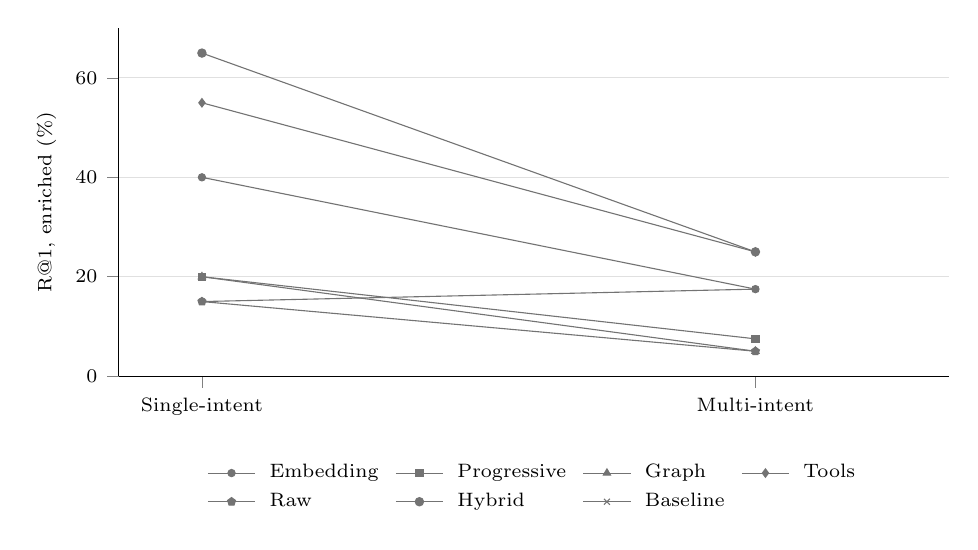
\begin{tikzpicture}
    \begin{axis}[
      width=\columnwidth, height=6.0cm,
      xmin=0.85, xmax=2.35,
      xtick={1,2}, xticklabels={Single-intent, Multi-intent},
      xticklabel style={font=\scriptsize},
      ymin=0, ymax=70,
      ytick={0,20,40,60}, yticklabel style={font=\scriptsize},
      ylabel={R@1, enriched (\%)}, ylabel style={font=\scriptsize},
      ymajorgrids, grid style={draw=black!12},
      axis y line*=left, axis x line*=bottom,
      tick align=outside,
      legend style={
        at={(0.5,-0.22)}, anchor=north, legend columns=4,
        draw=none, font=\scriptsize,
        /tikz/every even column/.append style={column sep=4pt},
        column sep=3pt,
      },
      legend cell align=left,
      cycle list={
        {black!55,mark=*,mark size=1.3pt},
        {black!55,mark=square*,mark size=1.3pt},
        {black!55,mark=triangle*,mark size=1.5pt},
        {black!55,mark=diamond*,mark size=1.5pt},
        {black!55,mark=pentagon*,mark size=1.5pt},
        {black!55,mark=otimes*,mark size=1.5pt},
        {black!55,mark=x,mark size=1.5pt},
      },
    ]
      \addplot coordinates {(1,40.0) (2,17.5)}; \addlegendentry{Embedding}
      \addplot coordinates {(1,20.0) (2,7.5)};  \addlegendentry{Progressive}
      \addplot coordinates {(1,20.0) (2,5.0)};  \addlegendentry{Graph}
      \addplot coordinates {(1,55.0) (2,25.0)}; \addlegendentry{Tools}
      \addplot coordinates {(1,15.0) (2,5.0)};  \addlegendentry{Raw}
      \addplot coordinates {(1,65.0) (2,25.0)}; \addlegendentry{Hybrid}
      \addplot coordinates {(1,15.0) (2,17.5)}; \addlegendentry{Baseline}
    \end{axis}
  \end{tikzpicture}
  \caption{R@1 drop from single-intent to multi-intent Dynamic cases under enrichment. Every retrieval method degrades sharply (H: $65\to25$, T: $55\to25$), because decomposing a multi-intent request multiplies per-sub-query errors. Only the no-retrieval baseline~B is flat, as it never decomposes.}
  \label{fig:intent-slope}
\end{figure}

\begin{table}[h]
  \renewcommand{\arraystretch}{1.0}
  \caption{Dynamic results ($n{=}40$: 20 single-intent + 20 multi-intent). Suffix 0 = without enrichment, 1 = with enrichment. $\Delta$ = enriched $-$ baseline. Tokens = avg.\ per case. R@1, R@5, $\Delta$R@1 in \% (pp for $\Delta$). Bold = best per column. $^{\dagger}$amortised embedding cost; $^{*}$agentic composite (H).}
  \label{tab:dy-results}
  \centering\footnotesize
  \setlength{\tabcolsep}{5pt}
  \begin{tabular}{@{} l cccc cc cc @{}}
  \toprule
  & \multicolumn{4}{c}{\textbf{Combined}} & \multicolumn{2}{c}{\textbf{Single-Intent}} & \multicolumn{2}{c}{\textbf{Multi-Intent}} \\
  \cmidrule(lr){2-5}\cmidrule(lr){6-7}\cmidrule(lr){8-9}
  \textbf{Meth.} & \textbf{R@1} & \textbf{R@5} & \textbf{$\Delta$R@1} & \textbf{Tok.} & \textbf{R@1} & \textbf{R@5} & \textbf{R@1} & \textbf{R@5} \\
  \midrule
  Baseline$_0$ & 16.3 & 46.3 & --- & 23{,}688 & 15.0 & 50.0 & 17.5 & 42.5 \\
  Baseline$_1$ & 16.3 & 46.3 & $\pm$0.0 & 23{,}688 & 15.0 & 50.0 & 17.5 & 42.5 \\
  \midrule
  Embedding$_0^{\dagger}$ & \textbf{32.5} & \textbf{67.5} & --- & \textbf{693} & \textbf{45.0} & \textbf{80.0} & \textbf{20.0} & \textbf{55.0} \\
  Embedding$_1^{\dagger}$ & 28.7 & \textbf{70.0} & $-3.8$ & \textbf{999} & 40.0 & \textbf{85.0} & 17.5 & \textbf{55.0} \\
  \midrule
  Progressive$_0$ & 13.8 & 28.7 & --- & 5{,}773 & 15.0 & 30.0 & 12.5 & 27.5 \\
  Progressive$_1$ & 13.8 & 27.5 & $\pm$0.0 & 6{,}292 & 20.0 & 30.0 & 7.5 & 25.0 \\
  \midrule
  Graph$_0$ & 2.5 & 7.5 & --- & 4{,}405 & 5.0 & 15.0 & 0.0 & 0.0 \\
  Graph$_1$ & 12.5 & 17.5 & $+10.0$ & 7{,}359 & 20.0 & 20.0 & 5.0 & 15.0 \\
  \midrule
  Tools$_0$ & 25.0 & 31.2 & --- & 39{,}760 & 35.0 & 45.0 & 15.0 & 17.5 \\
  Tools$_1$ & \textbf{40.0} & 48.7 & \textbf{$+15.0$} & 47{,}859 & \textbf{55.0} & 70.0 & \textbf{25.0} & 27.5 \\
  \midrule
  Raw$_0$ & 12.5 & 12.5 & --- & 71{,}235 & 25.0 & 25.0 & 0.0 & 0.0 \\
  Raw$_1$ & 10.0 & 10.0 & $-2.5$ & 52{,}117 & 15.0 & 15.0 & 5.0 & 5.0 \\
  \midrule
  Hybrid$_0^{*}$ & \textbf{42.5} & 51.2 & --- & 17{,}583 & \textbf{50.0} & 50.0 & \textbf{35.0} & 52.5 \\
  Hybrid$_1^{*}$ & \textbf{45.0} & 53.7 & $+2.5$ & 22{,}969 & \textbf{65.0} & 65.0 & \textbf{25.0} & 42.5 \\
  \bottomrule
  \end{tabular}
\end{table}


% ─────────────────────────────────────────────────────────────────────────────

\end{document}
